%% ============================================================================
%% AeroTray -- manuscrito con formato HardwareX, version final en espanol
%% (MT5001 Diseno de Sistemas Mecatronicos, UTEC, 2026-2)
%% Compilar con pdfLaTeX + BibTeX (opcion por defecto de Overleaf). Cada seccion
%% vive en sections/*.tex para que cada autor edite su parte sin conflictos.
%% Antes de entregar, buscar "TODO" y \tocheck{...}.
%% ============================================================================
\documentclass[preprint,12pt,a4paper]{elsarticle}
%% ======================================================================
%% preamble.tex -- paquetes y macros comunes a todas las secciones
%% ======================================================================
\usepackage{iftex}
\ifXeTeX
  \usepackage{fontspec}
\else
  \usepackage[T1]{fontenc}
  \usepackage[utf8]{inputenc}
  \usepackage{lmodern}
  \usepackage{textcomp}
\fi
%% Espanol: tablas como "Tabla", coma decimal automatica en modo matematico (0.14 -> 0,14),
%% sin atajos de comillas ni tilde para no romper tikz/hyperref.
\usepackage[spanish,es-tabla,es-nolists,es-noquoting,es-notilde,es-ucroman]{babel}
\usepackage{amsmath,amssymb,bm}
\usepackage{graphicx}
\usepackage{booktabs,tabularx,multirow,longtable,array}
\usepackage{siunitx}
\usepackage{xcolor}
%% Paleta comun con figuras_matlab/estilo_paper.m (Okabe-Ito adaptada)
\definecolor{pAzul}{HTML}{0072B2}
\definecolor{pRojo}{HTML}{D55E00}
\definecolor{pVerde}{HTML}{009E73}
\definecolor{pOcre}{HTML}{B07A00}
\definecolor{pMorado}{HTML}{A0529A}
\definecolor{pGris}{HTML}{6E6E6E}
\usepackage{tikz}
\usetikzlibrary{arrows.meta,positioning,shapes.geometric,fit,calc,backgrounds}
\usepackage{subcaption}
\usepackage[section]{placeins}
\usepackage{enumitem}
\usepackage[colorlinks=true,linkcolor=blue!50!black,citecolor=blue!50!black,urlcolor=blue!60!black]{hyperref}
\makeatletter\g@addto@macro{\UrlBreaks}{\do\_\do\-\do\.}\makeatother

\sisetup{detect-all, range-phrase = \text{--}, per-mode = symbol, output-decimal-marker = {,},
         list-pair-separator = {\text{ y }}, list-final-separator = {\text{ y }}}
\setlist{itemsep=1pt,topsep=3pt}
\setlength{\emergencystretch}{3em}
\renewcommand{\arraystretch}{1.15}

%% ---------------------------------------------------------------- macros
\newcommand{\fn}[1]{\path{#1}}
\newcommand{\repourl}{\url{https://github.com/geo105/AeroTray}}
\newcommand{\us}{\,\si{\micro\second}}
\newcommand{\Rot}{\mathbf{R}}
\newcommand{\vect}[1]{\bm{#1}}
\newcommand{\ez}{\vect{e}_z}
\newcommand{\skw}[1]{[#1]_\times}
\newcommand{\T}{^{\!\top}}
\newcommand{\dd}{\mathrm{d}}
\newcommand{\sat}{\operatorname{sat}}
\newcommand{\diag}{\operatorname{diag}}
%% editorial marks (remove before submission)
\newcommand{\tocheck}[1]{\textcolor{red}{#1}}

%% pie de la primera pagina en espanol (elsarticle lo trae en ingles)
\usepackage{etoolbox}
\makeatletter\patchcmd{\ps@pprintTitle}{Preprint submitted to}{Preprint enviado a}{}{}\makeatother

\journal{HardwareX}
\abstracttitle{Resumen}
\keywordtitle{Palabras clave}

\begin{document}

%% ======================================================================
%% 00_frontmatter.tex -- titulo, autores, resumen y palabras clave
%% ======================================================================
\begin{frontmatter}

% Titulo anterior: AeroTray: robot móvil abierto que transporta un octocóptero montado en una rótula y un \textit{ball and plate} con visión, con un modelo validado de la propagación de perturbaciones a través de etapas de equilibrio apiladas
\title{AeroTray: sistema \textit{ball and plate} sobre un octocóptero acoplado en una base móvil diferencial}

\author[utec]{Sebastián Rejas Córdova}
\ead{sebastian.rejas.c@utec.edu.pe}
\author[utec]{George Henry Ramos Astuhuamán\corref{cor1}}
\ead{george.ramos@utec.edu.pe}
\author[utec]{Johan Nireo Naupay Fabián}
\ead{johan.naupay@utec.edu.pe}
\author[utec]{Hideky Edu Garnique Pisfil}
\ead{hideky.garnique@utec.edu.pe}
\author[utec]{Diego André Miranda Zamora}
\ead{diego.miranda@utec.edu.pe}
\cortext[cor1]{Autor de correspondencia.}
\address[utec]{Departamento de Ingeniería Mecatrónica, Universidad de Ingeniería y Tecnología (UTEC), Jr. Medrano Silva 165, Barranco, Lima, Perú}

\begin{abstract}
AeroTray es una plataforma mecatrónica de tres niveles: una base diferencial (chasis TETRIX, NI myRIO-1900), un módulo aéreo de ocho rotores (\SI{3.6}{\kilo\gram}) montado sobre una rótula pasiva que desliza por una guía vertical de \SI{140}{\milli\metre}, y un \textit{ball and plate} de dos servos sobre el octocóptero, cuya bola sigue una cámara a \SI{187}{fps}. Cada maniobra de la base se propaga por la rótula al octocóptero y, a través de él, a la bola, de modo que la plataforma hace observable el acoplamiento entre problemas de equilibrio apilados. Publicamos todo el hardware y el software y deducimos un modelo de primeros principios de la cadena completa: la cinemática y la dinámica no holonómicas de la base en pendiente, la dinámica de Newton--Euler del octocóptero alrededor de un pivote acelerado, la asignación de control de los ocho rotores y las ecuaciones exactas de una bola que rueda sobre un plato que se traslada y rota, todas verificadas simbólicamente. A partir de la telemetría de vuelo estacionario identificamos, con un balance estático de momentos, la excentricidad del centro de masa ($9{,}5\pm1{,}8$\,mm) y su altura sobre la rótula ($0{,}14\pm0{,}06$\,m), y con la condición de despegue la ganancia real de empuje, 33--52\% mayor que la del mapa del firmware. El modelo justifica el uso del dron en la rampa: su actuador empuja contra el aire y no contra la base, de modo que, al nivelarse, desacopla la pendiente del plato (en la rampa los servos no trabajaron más que en llano); y al sostener parte de su propio peso baja el centro de masa, lo que eleva la pendiente de vuelco al subir de \SI{21.5}{\degree} (medida) a \SI{27.7}{\degree} (prevista por el modelo) con la mitad del peso del módulo en los rotores. El modelo explica cuantitativamente los hechos experimentales principales: las derivas lentas de actitud de los primeros vuelos (región de atracción por autoridad de par de solo 3--4$^\circ$), el periodo de la oscilación residual en vuelo estacionario (0,2--0,3\,Hz previsto; 0,15--0,23\,Hz medido), el límite de estabilidad del controlador de la bola (ganancia derivativa 4,5 estable, 6 inestable), la velocidad de la base en llano (0,072\,m/s prevista; 0,06--0,08\,m/s medida) y la pérdida de vuelo al descargarse las baterías: el colectivo de despegue sube de 1725--\SI{1775}{\micro\second} con 12,4\,V a 1850--\SI{2000}{\micro\second} con 11,1\,V, por encima del límite sostenido del firmware, lo que deja entre 3 y 7 minutos de vuelo útil por par de LiPo. Experimentalmente, el firmware final mantiene el octocóptero en la guía con 0,55--1,7$^\circ$ de error RMS de actitud, y el controlador de la bola la mantiene a una distancia mediana de 19\,mm del centro con la base quieta y los rotores girando, y de 28--30\,mm mientras el robot avanza en llano y por una rampa de 10$^\circ$. En los ensayos finales sobre el robot completo (23/11) se registraron 13 ensayos de equilibrio de 23--\SI{122}{\second} (\SI{816}{\second} en total; mediana de 29--44\,mm), 10 de ellos con los rotores encendidos y el dron nivelado a 0,71--1,0$^\circ$ RMS; en cuatro ensayos completos la base cruzó la rampa de 10$^\circ$ con la bola en equilibrio durante 18--\SI{30}{\second} (mediana de 30--35\,mm, dron a 0,85--1,15$^\circ$ RMS sin cortes, con la bola saliendo del plato en el tramo final), y el módulo despegó y aterrizó en la guía con la bandeja encima (la bola salió al despegar por el salto de fricción de la guía); el error restante se concentra en un desnivel del eje $x$ del plato. Se publican todos los archivos CAD, el firmware, los VI de LabVIEW, los scripts de análisis y los registros.
\end{abstract}

\begin{keyword}
Robot móvil \sep Banco de pruebas de octocóptero \sep \textit{Ball and plate} \sep Dinámica no holonómica \sep Propagación de perturbaciones \sep Identificación de sistemas \sep Visión por computadora \sep Educación
\end{keyword}

\end{frontmatter}
         % titulo, autores, resumen, palabras clave

%% ======================================================================
%% 01_specifications.tex -- tabla de especificaciones de HardwareX
%% ======================================================================
\section*{Tabla de especificaciones}
\noindent\begin{tabularx}{\textwidth}{@{}>{\raggedright\arraybackslash}p{0.27\textwidth}X@{}}
\toprule
Nombre del hardware & AeroTray (base móvil + octocóptero en rótula esférica + \textit{ball and plate} con visión) \\
Área temática & Ingeniería y ciencia de materiales; herramientas educativas y alternativas de código abierto a la infraestructura existente \\
Tipo de hardware & Ingeniería mecánica y ciencia de materiales; ingeniería eléctrica y ciencias de la computación (robótica, control) \\
Análogo comercial más cercano & Ningún producto comercial combina los tres niveles. Análogos parciales: Quanser 3 DOF Hover / Aero (bancos de actitud de multirrotores), Quanser 2 DOF Ball Balancer, kits de robot móvil TETRIX/myRIO. \\
Licencia de código abierto & Hardware (CAD, planos): CERN-OHL-S v2. Software, firmware y scripts de análisis: MIT. Documentación y datos: CC BY 4.0. \\
Costo del hardware & Aproximadamente USD 1460 (Tabla~\ref{tab:bom}); unos USD 680 si se reutilizan la myRIO-1900, el kit TETRIX y su batería disponibles en el laboratorio de la universidad. \\
Repositorio de archivos fuente & \repourl \\
\bottomrule
\end{tabularx}
      % tabla de especificaciones HardwareX
%% ======================================================================
%% 02_context.tex -- 1. El hardware en contexto
%% ======================================================================
\section{El hardware en contexto}
\label{sec:context}

Los sistemas de equilibrio, como el péndulo invertido, la bola y viga, el \textit{ball and plate} y el banco de actitud de multirrotores, son referencias estándar en la enseñanza y la investigación en control porque son inestables en lazo abierto, baratos e intuitivos a la vista \cite{astrom2008,hauser1992,awtar2002}. En HardwareX se han publicado versiones abiertas de estas referencias, por ejemplo el péndulo de varios brazos sobre un carro \cite{kaheman2023} y el péndulo doble de bajo costo con seguimiento por video \cite{myers2020}, junto con robots móviles educativos abiertos como ROBOTONT \cite{raudmae2023} y PlatROB \cite{balbuena2026}, y manipuladores y cabezas educativas como EduSCARA \cite{clark2026} y BEATRIX \cite{al2024}. Estas plataformas estudian un problema de equilibrio a la vez, sobre una base fija.

En robótica de campo el caso relevante es el opuesto: una carga que debe permanecer nivelada viaja sobre un vehículo que acelera, gira y sube pendientes, y el propio vehículo puede llevar una etapa estabilizada activamente. Son ejemplos los estabilizadores de cámara en vehículos terrestres, las bandejas estabilizadas para objetos delicados \cite{selvaggio2023} y los vehículos aéreos que equilibran una carga inestable \cite{hehn2011}. En estos sistemas la perturbación que genera la base se propaga por cada etapa; cada estabilizador atenúa una parte y añade su propia dinámica, retardos y saturaciones. Los proyectos anteriores del curso en nuestra universidad abordaron una sola etapa estabilizada (un cardán de dos ejes sobre un robot diferencial, que detectaba la bola con una pantalla resistiva o con una cámara). Hasta donde sabemos, no existe una plataforma abierta y documentada en la que la propagación a través de \emph{dos} etapas con control activo, una de ellas un vehículo aéreo, pueda medirse con registros sincronizados \emph{y} predecirse con un modelo validado.

\paragraph{Por qué un dron y no un cardán}
La pregunta natural es por qué la etapa intermedia es un octocóptero y no un cardán motorizado de dos ejes, que también nivelaría el plato. La respuesta cuantitativa está en la Sección~\ref{sec:porquedron}. Un cardán solo puede \emph{girar} la carga; el octocóptero, además de nivelarse con la misma ley de control, puede \emph{sostener su propio peso}. Esa fuerza vertical es la única de la plataforma que no pasa por el contacto rueda--suelo, y en la rampa cambia los límites de la base: con la mitad del peso del módulo en los rotores, la pendiente de vuelco estático al subir pasa de \SI{21.5}{\degree} (medida) a \SI{27.7}{\degree} (prevista), al bajar pasa de \SI{30.5}{\degree} (medida) a \SI{38.2}{\degree} (prevista), y el margen de aceleración en una pendiente de \SI{20}{\degree} se multiplica por 3,5. Al mismo tiempo, el dron es el caso más exigente para la etapa intermedia (péndulo invertido con retardo de actuadores y autoridad de par limitada), lo que convierte a la plataforma en un paso previo, medible y seguro, hacia la manipulación aérea en vuelo libre, que es la línea de investigación del grupo.

AeroTray cubre ese vacío con componentes comerciales. Sus aportes son:
\begin{enumerate}[label=(\roman*)]
  \item una arquitectura reproducible de tres niveles (base terrestre, octocóptero sobre una rótula esférica pasiva con guía vertical, \textit{ball and plate}) con interfaces documentadas entre tres controladores independientes (myRIO, ESP32, ESP32-S3) y un supervisor Raspberry Pi, y un sistema de alimentación con dominios aislados y paro de emergencia (Sección~\ref{sec:description});
  \item un modelo cinemático y dinámico de primeros principios de toda la cadena, desde la velocidad de las ruedas hasta la aceleración de la bola, que incluye la base no holonómica en pendiente, el octocóptero como péndulo invertido sobre un pivote acelerado, la asignación de control de ocho rotores y las ecuaciones exactas de una bola que rueda sobre un plato que se traslada y rota; cada ecuación se verificó simbólicamente (Sección~\ref{sec:model} y \ref{app:derivations});
  \item un conjunto de resultados basados en el modelo que explican el comportamiento del prototipo: la identificación del centro de masa del módulo aéreo con telemetría de vuelo estacionario, la justificación cuantitativa del dron en la rampa (vuelco, par y tracción frente a la fracción de peso sostenida), el margen de empuje y la autonomía frente a la tensión de la batería, un mapa de estabilidad del lazo de actitud, una región de atracción por autoridad de par, el límite de estabilidad del lazo de la bola con retardo, la transmisibilidad de las aceleraciones de la base a la bola y los límites de vuelco estático y dinámico de la base (Secciones~\ref{sec:porquedron}--\ref{sec:modelval});
  \item firmware abierto para un controlador de actitud de octocóptero con modo de vuelo en guía, enclavamientos de seguridad y registro a bordo, un controlador de la bola con visión a \SI{187}{fps} en una Raspberry Pi 3B+, y una validación cuantitativa que incluye las iteraciones fallidas, la comparación con el modelo de Isaac Lab usado durante el diseño \cite{mittal2023,schulman2017}, los videos de vuelo sincronizados con la telemetría y todos los datos crudos (Sección~\ref{sec:validation}).
\end{enumerate}
La plataforma está pensada para enseñar integración, modelado y validación en diseño mecatrónico, y como banco de pruebas para controladores en cascada, basados en aprendizaje y con prealimentación de perturbaciones frente a las perturbaciones que induce la base.
             % 1. El hardware en contexto
%% ======================================================================
%% 03_description.tex -- 2. Descripcion del hardware (arquitectura, alimentacion, pines, decisiones)
%% ======================================================================
\section{Descripción del hardware}
\label{sec:description}

\subsection{Arquitectura}
La Fig.~\ref{fig:overview} muestra el prototipo final y su modelo CAD, y la Fig.~\ref{fig:architecture} su arquitectura eléctrica y de comunicaciones. El robot se organiza en cuatro subsistemas (tres niveles mecánicos y la electrónica auxiliar):

\begin{figure}[!htbp]
  \centering
  \begin{subfigure}[b]{0.43\textwidth}\centering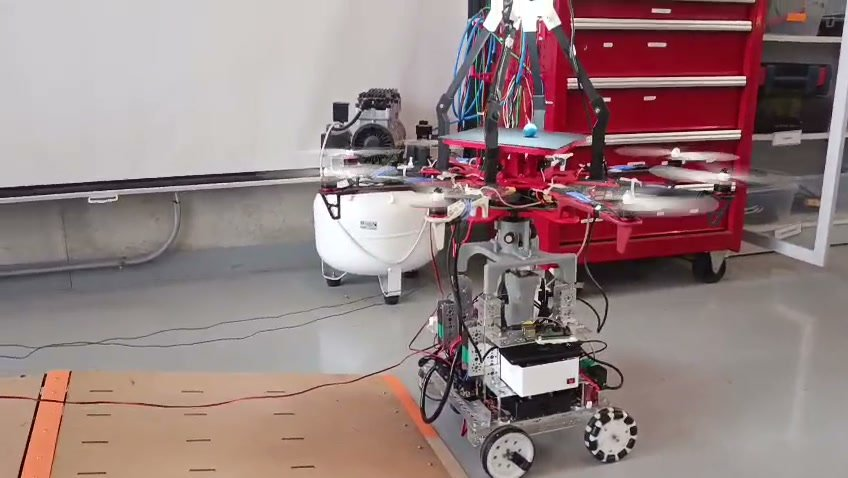
\includegraphics[width=\linewidth]{figures/photo_robot_side.jpg}\caption{Prototipo integrado.}\end{subfigure}\hfill
  \begin{subfigure}[b]{0.30\textwidth}\centering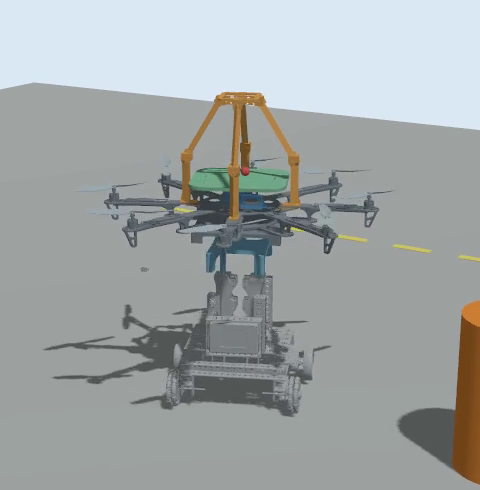
\includegraphics[width=\linewidth]{figures/cad_assembly.png}\caption{Ensamble CAD (383 piezas).}\end{subfigure}\hfill
  \begin{subfigure}[b]{0.25\textwidth}\centering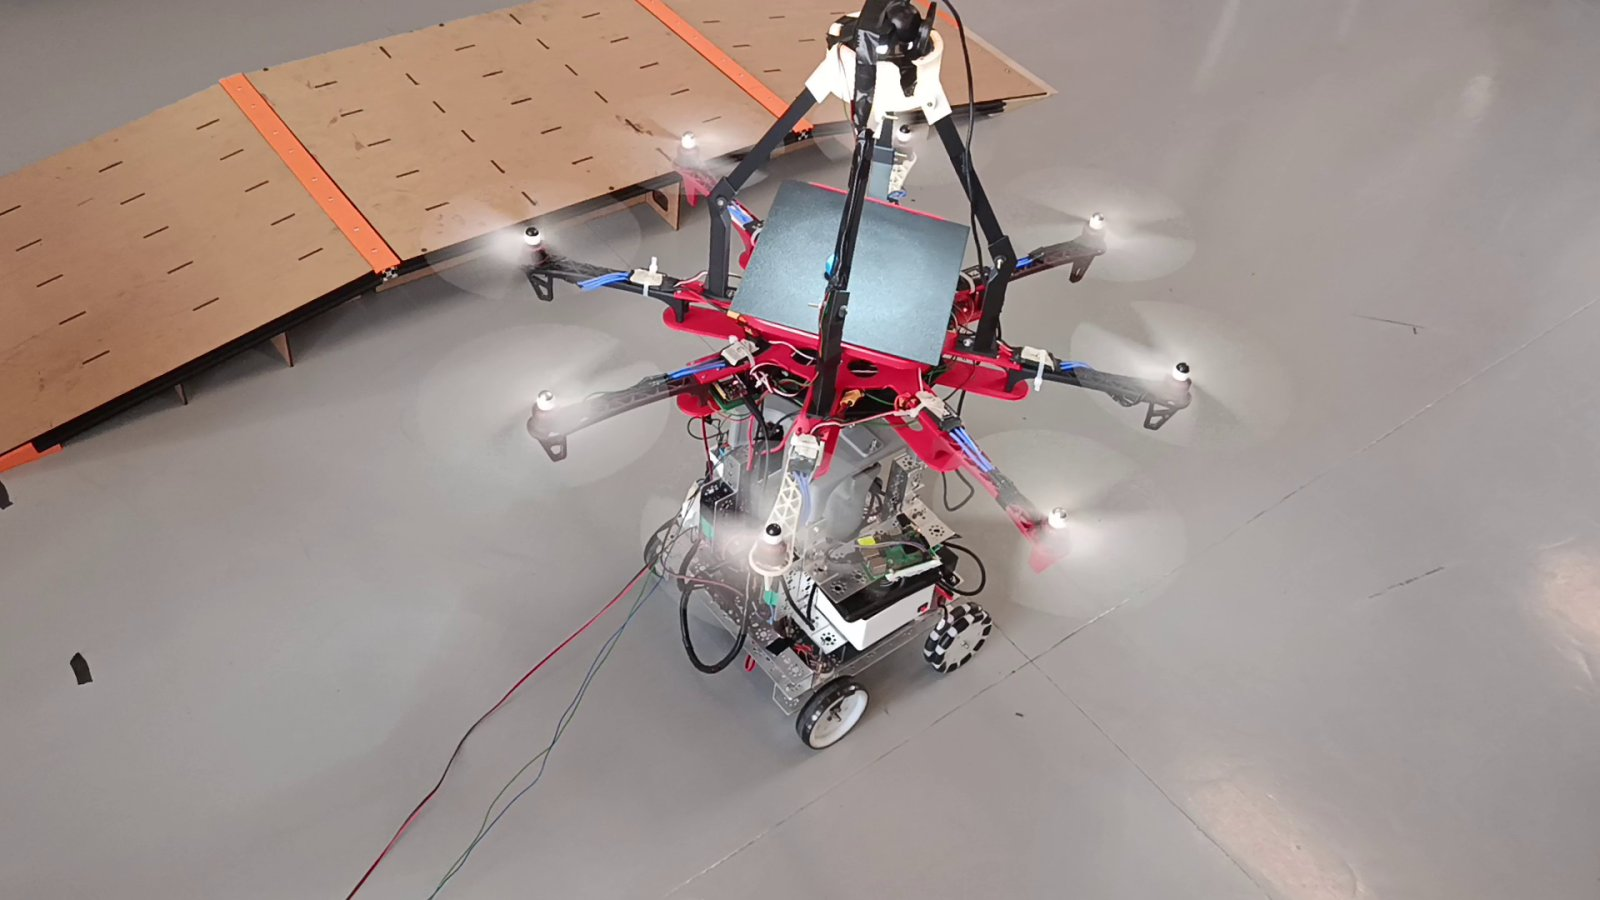
\includegraphics[width=\linewidth,trim=420 0 420 0,clip]{figures/photo_ramp_top.jpg}\caption{Sobre la rampa de \SI{10}{\degree}.}\end{subfigure}
  \caption{AeroTray. De abajo hacia arriba: base diferencial TETRIX con la myRIO, mástil con guía vertical, rótula esférica, octocóptero (marco rojo, ocho rotores) y bandeja del \textit{ball and plate} con la cámara cenital. La bola azul tiene \SI{27}{\milli\metre} de diámetro.}
  \label{fig:overview}
\end{figure}

\begin{enumerate}[label=\textbf{N\arabic*.}]
  \item \textbf{Base móvil.} Chasis de aluminio TETRIX MAX con dos ruedas motrices (motores DC TETRIX TorqueNADO con encoders en cuadratura) y dos ruedas omnidireccionales como apoyos pasivos. Una NI myRIO-1900 lee los encoders, calcula la odometría y ejecuta un lazo PI de velocidad por rueda; un puente H MDD10A alimenta los motores desde una batería NiMH TETRIX de \SI{12}{\volt}. Trocha $b=\SI{0.3794}{\metre}$; avance de la rueda por cuenta de encoder \SI{0.2151}{\milli\metre} (radio de rueda $r\approx\SI{49.3}{\milli\metre}$).
  \item \textbf{Módulo aéreo.} Octocóptero con brazos de radio $L=\SI{0.350}{\metre}$ (un motor cada \SI{45}{\degree}), ocho motores sin escobillas A2212 de 920\,KV con hélices 9450 y ESC de 30\,A sin BEC, dos baterías LiPo 3S de \SI{3300}{\milli\ampere\hour} (una por cada grupo de cuatro ESC), una IMU MPU-6050 y un sensor de tiempo de vuelo VL53L0X que mide la distancia a un blanco blanco mate fijo en la base (Sección~\ref{sec:altura}). Una NodeMCU-32S (ESP32) ejecuta el control de actitud a \SI{200}{\hertz}. El módulo se une al mástil mediante una rótula esférica montada en un carro que desliza por una guía vertical (recorrido medido de unos \SI{140}{\milli\metre}); la rótula deja libres el alabeo y el cabeceo y, por su fricción y sus topes, solo permite un giro pequeño de guiñada, de modo que el octocóptero gira con la base. El conjunto móvil pesa \SI{3.6}{\kilo\gram} (\SI{3.3}{\kilo\gram} el conjunto que rota y \SI{0.3}{\kilo\gram} el carro). El plano de los rotores está \SI{95}{\milli\metre} sobre el centro de la rótula.
  \item \textbf{Bandeja del \textit{ball and plate}.} Plato de $\SI{250}{\milli\metre}\times\SI{220}{\milli\metre}$ apoyado en su centro sobre una junta universal (cruceta) en un pilar fijo a la placa central del octocóptero, \SI{104}{\milli\metre} sobre la rótula, e inclinado en dos ejes por dos servos Futaba S3003 mediante mecanismos de cuatro barras (Sección~\ref{sec:linkage}). Una ESP32-S3 genera los pulsos de \SI{50}{\hertz} de los servos (GPIO47 para $x$, GPIO21 para $y$) y ejecuta el PID de la bola. Una cámara PS3 Eye, sostenida a $\approx$\SI{0.20}{\metre} sobre el plato por cuatro torres fijas al octocóptero (no al plato), envía cuadros de $320\times240$ a \SI{187}{fps} a la Raspberry Pi, que detecta la bola y envía su posición y velocidad a la ESP32-S3.
  \item \textbf{Supervisor, distribución electrónica y paro.} La Raspberry Pi 3B+ centraliza la visión, los enlaces y el registro, con dominios separados de lógica y paro de emergencia (Sección~\ref{sec:power}). En el módulo aéreo, las dos controladoras van debajo de la placa central, en brazos opuestos, para repartir el peso y separar el ruido de los ESC: la NodeMCU-32S (control de actitud) en el brazo 8 ($+x$) y la ESP32-S3 (bandeja) en el brazo 6 ($-x$). La IMU MPU-6050 y el láser VL53L0X están junto a la NodeMCU en el brazo 8, en el mismo bus I$^2$C. El láser apunta hacia abajo, al blanco fijo en la base. Por eso ambos sensores están desplazados del eje de la rótula, y la Sección~\ref{sec:altura} corrige la medida de altura por ese brazo de palanca.
\end{enumerate}

\begin{figure}[!htbp]
\centering
\begin{tikzpicture}[font=\footnotesize, >=Latex,
  colhdr/.style={font=\footnotesize\bfseries, text=pGris!85!black, align=center},
  blk/.style={draw, rounded corners=2pt, align=center, minimum height=11.5mm, inner xsep=2pt, inner ysep=2.5pt, line width=0.6pt},
  blkusr/.style={blk, fill=white, draw=pGris, text width=3.34cm},
  blkpw/.style={blk, fill=pRojo!7, draw=pRojo, text width=3.34cm},
  blkcp/.style={blk, fill=pAzul!7, draw=pAzul, text width=3.34cm},
  blksa/.style={blk, fill=pVerde!7, draw=pVerde, text width=4.04cm},
  pw/.style={->, line width=1.05pt, pRojo, rounded corners=2pt},
  pwbr/.style={pw, preaction={-, draw=white, line width=2.6pt, rounded corners=2pt}},
  dt/.style={<->, line width=0.85pt, pAzul, rounded corners=2pt},
  dt1/.style={->, line width=0.85pt, pAzul, rounded corners=2pt},
  lab/.style={font=\footnotesize, text=pAzul!90!black, inner sep=1.5pt}]
  % Coordenadas de las 3 columnas (ancho total = 13.38 cm < 13.74 cm = \textwidth)
  % Col 1: x=1.74 ([0.00, 3.48]), Col 2: x=6.28 ([4.54, 8.02]), Col 3: x=11.24 ([9.15, 13.33])
  \node[colhdr] at (1.74, -0.84) {Alimentación};
  \node[colhdr] at (6.28, 0.90) {Cómputo};
  \node[colhdr] at (11.24, 0.90) {Sensores y actuadores};

  % ---- Fila 1 (y = 0.00) -- todas las cajas de exactamente 2 lineas y mismo alto
  \node[blkusr] (web)  at (1.74,  0.00) {\textbf{Navegador}\\ laptop o celular};
  \node[blkcp]  (pi)   at (6.28,  0.00) {\textbf{Raspberry Pi 3B+}\\ visión, registro y web};
  \node[blksa]  (cam)  at (11.24, 0.00) {\textbf{Cámara PS3 Eye}\\ 320$\times$240 a 187 fps};

  % ---- Fila 2 (y = -1.68)
  \node[blkpw]  (pipw) at (1.74, -1.68) {\textbf{BT5: 3S 18650}\\ XL4015 $\to$ 5,2 V};
  \node[blkcp]  (s3)   at (6.28, -1.68) {\textbf{ESP32-S3}\\ PID de la bola};
  \node[blksa]  (srv)  at (11.24,-1.68) {\textbf{2$\times$ Futaba S3003}\\ servos de la bandeja};

  % ---- Fila 3 (y = -3.36)
  \node[blkpw]  (bt6)  at (1.74, -3.36) {\textbf{BT6: 3S 18650}\\ 5,2 V (servos, SB1)};
  \node[blksa]  (imu)  at (11.24,-3.36) {\textbf{MPU-6050, VL53L0X}\\ IMU y láser de altura};

  % ---- Fila 4 (y = -5.04)
  \node[blkpw]  (lipo) at (1.74, -5.04) {\textbf{2$\times$ LiPo 3S}\\ fus. 30 A, K1 y K2};
  \node[blkcp]  (nm)   at (6.28, -5.04) {\textbf{NodeMCU-32S}\\ actitud a 200 Hz};
  \node[blksa]  (esc)  at (11.24,-5.04) {\textbf{8$\times$ ESC 30 A}\\ y motores del dron};

  % ---- Fila 5 (y = -7.08)
  \node[blkpw]  (bt4)  at (1.74, -7.08) {\textbf{BT4: power bank}\\ 5 V $\to$ elevador 12 V};
  \node[blkcp]  (rio)  at (6.28, -7.08) {\textbf{NI myRIO-1900}\\ odometría y lazo PI};
  \node[blksa]  (hb)   at (11.24,-7.08) {\textbf{Puente H MDD10A}\\ 2$\times$TorqueNADO y enc.};

  % ---- Fila 6 (y = -8.68)
  \node[blkpw]  (nimh) at (1.74, -8.68) {\textbf{NiMH 12 V}\\ TETRIX, 20 A, K3};

  % ---- Enlaces de datos (azul #0072B2)
  \draw[dt]  ([yshift=2.2mm]web.east) -- node[lab, above=1.5pt]{Wi-Fi} ([yshift=2.2mm]pi.west);
  \draw[dt]  (pi.east) -- node[lab, above=1.5pt]{USB} (cam.west);
  \draw[dt]  ([xshift=3mm]pi.south) -- node[lab, right=2pt]{USB} ([xshift=3mm]s3.north);
  \draw[dt1] (s3.east) -- node[lab, above=1.5pt]{PWM} (srv.west);

  % Pi <-> NodeMCU (USB) por corredor izquierdo de Col 2 y celda libre Fila 3
  \draw[dt] ([xshift=-9mm]pi.south) -- ++(0,-0.42) -| (4.35,-3.36)
            -- node[lab, above=1.5pt, pos=0.55]{USB} (6.28,-3.36) -- (nm.north);
  % Pi <-> myRIO (UART 9600) por corredor paralelo y pasillo libre sobre myRIO
  \draw[dt] ([xshift=-13mm]pi.south) -- ++(0,-0.20) -| (3.98,-6.24)
            -- node[lab, above=1.5pt, pos=0.60]{UART 9600} (6.28,-6.24) -- (rio.north);

  % NodeMCU <-> IMU+VL53 (I2C) y NodeMCU -> ESC (PWM)
  \draw[dt]  ([xshift=10mm]nm.north) |- (8.05,-3.36) -- node[lab, above=1.5pt]{I$^2$C} (imu.west);
  \draw[dt1] (nm.east) -- node[lab, above=1.5pt]{PWM} (esc.west);
  % myRIO <-> MDD10A+TorqueNADO (PWM y encoders)
  \draw[dt1] ([yshift=2mm]rio.east) -- node[lab, above=1.5pt]{PWM} ([yshift=2mm]hb.west);
  \draw[dt1] ([yshift=-2mm]hb.west) -- node[lab, below=1.5pt]{enc.} ([yshift=-2mm]rio.east);

  % ---- Enlaces de alimentacion (rojo #D55E00)
  \draw[pw]   (pipw.east) -- (3.72,-1.68) |- ([yshift=-2.4mm]pi.west);
  \draw[pwbr] (bt6.east)  -- (3.72,-3.36) |- (3.72,-2.52) -| (srv.south);
  \draw[pwbr] (lipo.east) -- (3.72,-5.04) |- (3.72,-5.82) -| (esc.south);
  \draw[pw]   (bt4.east)  -- (rio.west);
  \draw[pw]   (nimh.east) -| (hb.south);

  % ---- Leyenda dentro de la figura (centrada debajo de la Fila 6)
  \node[draw=pGris!60, rounded corners=2pt, fill=white, inner xsep=6pt, inner ysep=4pt, anchor=north]
    (leg) at (6.66,-9.48) {%
    \begin{tikzpicture}[baseline=-0.5ex, font=\footnotesize]
      \draw[dt]  (0.00,0) -- (0.58,0); \node[right=2.5pt, inner sep=0pt] at (0.58,0) {Datos};
      \draw[pw]  (1.75,0) -- (2.33,0); \node[right=2.5pt, inner sep=0pt] at (2.33,0) {Alimentación};
      \draw[fill=pRojo!7,  draw=pRojo,  rounded corners=1pt] (4.70,-0.12) rectangle (5.00,0.12);
      \node[right=2.5pt, inner sep=0pt] at (5.00,0) {Fuentes};
      \draw[fill=pAzul!7,  draw=pAzul,  rounded corners=1pt] (6.52,-0.12) rectangle (6.82,0.12);
      \node[right=2.5pt, inner sep=0pt] at (6.82,0) {Cómputo};
      \draw[fill=pVerde!7, draw=pVerde, rounded corners=1pt] (8.52,-0.12) rectangle (8.82,0.12);
      \node[right=2.5pt, inner sep=0pt] at (8.82,0) {Sensores y actuadores};
    \end{tikzpicture}};
\end{tikzpicture}
\caption{Arquitectura eléctrica y de comunicaciones. Los dominios de alimentación solo comparten la tierra a través de los cables de señal; la Raspberry Pi alimenta por USB a la cámara, la ESP32-S3 y la NodeMCU-32S. La asignación de pines figura en la Tabla~\ref{tab:pins} y las tramas en la Sección~\ref{sec:interfaces}.}
\label{fig:architecture}
\end{figure}

\subsection{Sistema de alimentación y paro de emergencia}
\label{sec:power}
La alimentación sigue el esquema eléctrico Rev.~I (18/11/2026), que se publica con los archivos de diseño, y la auditoría de alimentación del grupo. Hay cinco dominios con fuente propia que solo se unen por la tierra de señal de los cables PWM y USB:
\begin{enumerate}[label=\textbf{S\arabic*.}]
  \item \textbf{Propulsión del dron, dos ramas aisladas.} Cada LiPo 3S \SI{3300}{\milli\ampere\hour} 25C (BT1, BT2) pasa por un conector XT60, un fusible ATO de \SI{30}{\ampere} (F1, F2) y el contacto 30--87 de un relé automotriz (K1, K2), y sube al dron por un cable 14\,AWG de $\approx$\SI{1}{\metre} (resistencia de lazo \SI{16.6}{\milli\ohm}) hasta un condensador de \SI{1000}{\micro\farad}/\SI{25}{\volt} por nodo. La rama A alimenta los ESC 1, 3, 5 y 7 (M1, M3, M5, M7) y la rama B los ESC 2, 4, 6 y 8. Cada rama tiene dos pares opuestos con dos motores de cada sentido de giro, así que una batería más descargada que la otra reduce el empuje total pero no produce par de guiñada. Los negativos A$-$ y B$-$ solo se unen en el dron (GND\_D) y el cable rojo de BEC de los ESC está cortado.
  \item \textbf{Base TETRIX.} NiMH \SI{12}{\volt} \SI{3000}{\milli\ampere\hour} (BT3), fusible interno de \SI{20}{\ampere} y relé K3, hacia el puente H MDD10A ($2\times\SI{10}{\ampere}$) y los dos TorqueNADO.
  \item \textbf{myRIO.} Power bank de \SI{5}{\volt}/\SI{3}{\ampere} (BT4) y elevador de 5 a \SI{12}{\volt}; la myRIO alimenta los encoders.
  \item \textbf{Lógica de \SI{5}{\volt}} (raíz del árbol de tierras). Pack 3S de celdas 18650 con BMS (BT5), fusible de \SI{3}{\ampere}, interruptor SW1 y regulador XL4015 a \SI{5.2}{\volt}; alimenta la Raspberry Pi y, por el hub USB, la NodeMCU-32S con sus sensores y la ESP32-S3.
  \item \textbf{Servos y paro.} Segundo pack 3S 18650 con BMS (BT6), fusible de \SI{3}{\ampere}, SW2 y XL4015 hacia los dos S3003 (con \SI{1000}{\micro\farad} y $2\times\SI{100}{\micro\farad}$) y el aro LED. Desde el mismo pack, por un fusible de \SI{1}{\ampere} y un cable mellizo de \SI{4}{\metre}, se alimentan las bobinas de K1--K4 a través del hongo de emergencia SB1 (normalmente cerrado y enclavable) de la caja de mando; las bobinas llevan diodos 1N4007 de rueda libre. Al pulsar SB1 se abren a la vez las dos ramas de la LiPo, la batería de la base y la alimentación de los servos (K4), mientras la lógica sigue encendida y registrando.
\end{enumerate}
En vuelo estacionario cada rama entrega 18--\SI{22}{\ampere} (60--75\% del fusible; Sección~\ref{sec:bateria}). Por encima de \SI{1850}{\micro\second} la corriente se acerca a los \SI{30}{\ampere}, por eso el firmware limita ese tramo a \SI{20}{\second}. El esquema Rev.~I indica que no hay medición de baterías: aunque el conexionado Rev.~E dibuja divisores de \SI{10}{\kilo\ohm}/\SI{3.3}{\kilo\ohm} hacia GPIO34 y GPIO35, el firmware v11 no los lee, y la tensión de las LiPo se mide a mano antes y después de cada sesión (Sección~\ref{sec:operation}).

\subsection{Asignación de pines}
\label{sec:pins}
Algunos documentos del proyecto (diagramas anteriores y la propuesta de la auditoría de mover ESC4 y ESC7) no coinciden con el código. La Tabla~\ref{tab:pins} toma como referencia el firmware publicado en \fn{03_firmware}, que es el que vuela.

\begin{table}[!htbp]
\centering
\caption{Pines de los controladores embebidos según el firmware que vuela: v11 del dron y PID de la bola en la ESP32-S3 (carpeta \texttt{03\_firmware}).}
\label{tab:pins}
\small
\begin{tabularx}{\textwidth}{@{}llX@{}}
\toprule
Controlador & Pin & Función \\
\midrule
NodeMCU-32S (U10) & GPIO25, 27, 21, 5 & PWM \SI{50}{\hertz} de M1, M3, M5, M7 (rama A) \\
 & GPIO26, 14, 19, 17 & PWM \SI{50}{\hertz} de M2, M4, M6, M8 (rama B) \\
 & GPIO23 / GPIO22 & I$^2$C SDA / SCL a \SI{100}{\kilo\hertz}: MPU-6050 (0x68) y VL53L0X (0x29) \\
 & GPIO34 / GPIO35 & VBAT\_A / VBAT\_B por divisor $\div4{,}03$ (cableado en Rev.~E; no usado por el firmware v11) \\
 & USB & \SI{5}{\volt}, órdenes, latido y telemetría con la Raspberry Pi \\
ESP32-S3 (U16) & GPIO47 / GPIO21 & pulso del servo $x$ / servo $y$ (\SI{50}{\hertz}, neutros 1386/\SI{1392}{\micro\second}, $\pm\SI{220}{\micro\second}$) \\
Raspberry Pi 3B+ & GPIO14 / GPIO15 & UART TX / RX hacia MXP-A pin 10 (RX) / pin 14 (TX) de la myRIO, 9600 8N1 \\
myRIO-1900 & MXP-A, MXP-B & PWM y DIR hacia el MDD10A y entradas de encoder (motor izquierdo en MXP-A, derecho en MXP-B); UART en MXP-A \\
\bottomrule
\end{tabularx}
\end{table}

GPIO5 y GPIO14 emiten pulsos durante el arranque del ESP32. Mientras sigan en esos pines, las ramas de la LiPo se energizan (se suelta SB1 y cierran K1 y K2) solo después de que la NodeMCU arrancó y envía \SI{1000}{\micro\second} a todos los ESC.

\subsection{Supervisor e interfaces}
\label{sec:interfaces}
La Raspberry Pi 3B+ es el centro del sistema. Su programa (\texttt{seguidor.py}) cumple cinco funciones:
\begin{itemize}
  \item captura la PS3 Eye en YUYV crudo a \SI{187}{fps}, rectifica el plato con una homografía calculada con sus cuatro esquinas y detecta la bola por color con OpenCV \cite{bradski2000};
  \item reenvía la posición y la velocidad de la bola a la ESP32-S3 por serie USB (trama \texttt{p x,y,vx,vy});
  \item intercambia órdenes, un latido (\texttt{hb}) y telemetría con el octocóptero por serie USB;
  \item se comunica con la myRIO por la UART física del conector GPIO;
  \item registra todo en archivos CSV y sirve tres páginas web, \texttt{/} (\textit{ball and plate}), \texttt{/dron} (octocóptero) y \texttt{/robot} (robot completo).
\end{itemize}
La myRIO y la Pi intercambian dos tramas de texto a 9600\,baudios, 8N1:
\begin{itemize}
  \item de la myRIO a la Pi, \texttt{cmd1,cmd2}, donde los códigos 1--4 son órdenes del octocóptero y los códigos 5--11 son órdenes del \textit{ball and plate};
  \item de la Pi a la myRIO, cada \SI{50}{\milli\second}, \texttt{x,y,roll,pitch,uav,bp}.
\end{itemize}
Las órdenes recibidas de la myRIO tienen prioridad sobre las órdenes web durante \SI{250}{\milli\second}.

\subsection{Decisiones de diseño y modificaciones}
La configuración final es el resultado de varias iteraciones; las decisiones más relevantes son:
\begin{itemize}
  \item \textbf{Un dron sobre la base, y no un cardán.} El octocóptero cumple dos funciones que un cardán motorizado no puede cumplir a la vez: se nivela respecto a la gravedad, lo que elimina la pendiente del suelo de la dinámica de la bola (Sección~\ref{sec:chain}), y sostiene parte de su propio peso, lo que en la rampa baja el centro de masa efectivo del robot y reduce el par de subida (Sección~\ref{sec:porquedron}).
  \item \textbf{Rótula pasiva en lugar de vuelo libre.} Una rótula esférica sobre una guía vertical deja que el octocóptero se equilibre en alabeo y cabeceo y suba unos centímetros, pero lo mantiene cautivo; eso es seguro en interiores y conserva el acoplamiento mecánico con la base que estudia el proyecto.
  \item \textbf{Ocho rotores.} Con 8 motores el conjunto de \SI{3.6}{\kilo\gram} flota con baterías cargadas a 1725--\SI{1775}{\micro\second} (68--74\% del recorrido útil del mapa) y el mezclador puede intercambiar empuje colectivo por par de actitud (Sección~\ref{sec:aerial}). El margen de empuje depende fuertemente de la tensión de la batería (Sección~\ref{sec:bateria}).
  \item \textbf{Cámara en la Pi en lugar de una cámara en la ESP32.} La primera versión usaba una cámara en la ESP32-S3, limitada a unos 50\,fps por la compresión JPEG (con menor calidad JPEG aparecían cientos de cuadros corruptos por minuto). El cambio a una PS3 Eye en la Pi subió la tasa a \SI{187}{fps} con cuadros sin comprimir, lo que volvió utilizables la estimación de velocidad y el término derivativo del PID de la bola; el retardo que queda en el lazo es lo que limita la ganancia derivativa (Sección~\ref{sec:ballcontrol}).
  \item \textbf{Dominios de alimentación separados.} Cada subsistema tiene su fuente y los dominios solo comparten la tierra (Sección~\ref{sec:power}). El BMS original de servos y bobinas falló durante el proyecto; en parte de los ensayos se reemplazó por una fuente de banco (Sección~\ref{sec:limits}).
  \item \textbf{Iteraciones del firmware de vuelo.} Nueve vuelos en la guía llevaron al firmware v9 (Sección~\ref{sec:flights}): filtro pasabajos del acelerómetro contra la vibración de los rotores, lazo activo de guiñada, integral de ángulo mayor, límite más amplio de la orden de velocidad angular en vuelo e histéresis en las ganancias de vuelo. El modelo de la Sección~\ref{sec:authority} explica por qué el cambio decisivo fue el límite de la orden de velocidad angular y no las ganancias. La versión final v11 añadió una ventana deslizante de guiñada en ralentí para los giros de la base y un filtro de Kalman con control de altura en cascada sobre el láser calibrado (Sección~\ref{sec:altura}).
\end{itemize}
         % 2. Descripcion del hardware (incluye alimentacion y pines)
%% ======================================================================
%% 04a_kinematics.tex -- 3. Modelo (parte 1): supuestos, marcos, parametros, cinematica
%% Verificacion simbolica: scripts_modelo/derive_*.py ; cifras: scripts_modelo/analysis.py
%% ======================================================================
\section{Modelo cinemático y dinámico}
\label{sec:model}

Esta sección deduce el modelo de la cadena completa, base $\to$ rótula $\to$ octocóptero $\to$ plato $\to$ bola, que se usó para dimensionar el prototipo, para diseñar y diagnosticar sus tres controladores y para interpretar los experimentos de la Sección~\ref{sec:validation}. La deducción va de abajo hacia arriba: supuestos, marcos y parámetros (Sección~\ref{sec:assumptions}); cinemática de la base, de la cadena y del accionamiento del plato (Secciones~\ref{sec:basekin}--\ref{sec:linkage}); dinámica de la base, del octocóptero y de la bola (Secciones~\ref{sec:basedyn}--\ref{sec:ball}); la justificación del dron en la rampa y su margen de empuje frente a la batería (Secciones~\ref{sec:porquedron}--\ref{sec:bateria}); y, por último, el modelo lineal acoplado, los controladores y las limitaciones fundamentales que se siguen de él (Secciones~\ref{sec:coupling}--\ref{sec:limits_fund}). Cada ecuación de la dinámica de la bola y del octocóptero se verificó simbólicamente con SymPy, y cada cifra de esta sección la calculan los scripts de \fn{scripts_modelo/} del repositorio (\ref{app:derivations}).

\subsection{Supuestos, marcos y parámetros}
\label{sec:assumptions}

\paragraph{Supuestos de modelado}
\begin{enumerate}[label=\textbf{A\arabic*.}, leftmargin=*]
  \item Todos los eslabones son rígidos. Se desprecia la flexibilidad de las placas y torres de PLA.
  \item Las ruedas motrices ruedan sin deslizamiento longitudinal ni lateral; las ruedas omnidireccionales son apoyos pasivos con resistencia lateral despreciable.
  \item La rótula esférica es ideal en alabeo y cabeceo; su par de fricción $\vect{\tau}_f$ se trata como una perturbación no modelada. Su guiñada queda bloqueada por fricción y por los topes, de modo que el rumbo del octocóptero sigue al de la base (lo confirman los cortes por guiñada de la Sección~\ref{sec:integrated}).
  \item La guía vertical es una articulación prismática con fricción de Coulomb y viscosa $F_g(\dot d)$ y topes rígidos en $d=0$ y $d=d_{\max}$.
  \item Cada rotor produce un empuje $F_i$ según $+\vect{z}_D$ y un par de reacción proporcional a él; el conjunto ESC--motor--hélice responde a su orden con un retardo puro seguido de un retraso de primer orden $\tau_m$. El empuje a orden fija escala con el cuadrado de la tensión que llega a los ESC (Sección~\ref{sec:bateria}).
  \item La bola es una esfera homogénea que rueda sin deslizar; se desprecia su resistencia a la rodadura. El factor de inercia $\gamma_b=1/(1+I_b/m_br_b^2)$ se mantiene general ($\gamma_b=5/7$ para una esfera maciza, $3/5$ para un cascarón delgado).
  \item Los servos son servos de posición con un retardo puro y un retraso de primer orden; el juego del mecanismo se trata como una no linealidad fuera del modelo lineal.
  \item Para el análisis lineal, los ángulos, las velocidades angulares y las aceleraciones son pequeños y la base se mueve con inclinación constante salvo en las transiciones de la rampa.
\end{enumerate}

\paragraph{Marcos y notación}
Los marcos se muestran en la Fig.~\ref{fig:frames}. $\{W\}$ es un marco inercial con $\vect z_W$ hacia arriba. $\{B\}$ está unido a la base, con origen en el suelo bajo el punto medio del eje motriz (trasero), $\vect x_B$ hacia adelante (hacia las ruedas omnidireccionales) y $\vect z_B$ normal al suelo. $\{J\}$ tiene su origen en el centro de la rótula esférica, a una altura $h_{J0}+d$ sobre el suelo y a una distancia $\ell_J$ por delante del eje motriz, donde $d\in[0,d_{\max}]$ es el desplazamiento en la guía. $\{D\}$ está fijo al octocóptero con origen en el centro de la rótula, $\vect x_D$ hacia el motor M8, $\vect y_D$ hacia el motor M7 y $\vect z_D$ hacia arriba (convención FLU del firmware). $\{G\}$ está fijo al octocóptero en el centro de la junta universal del plato, a una altura $h_P$ según $\vect z_D$. $\{P\}$ es el marco del plato, con origen en el centro de la junta universal; el centro de la bola tiene coordenadas $\vect\rho=[x_b,\,y_b,\,\varepsilon]\T$ en $\{P\}$, donde $\varepsilon$ es la altura del centro de la bola sobre el centro de la junta universal. $\Rot_x,\Rot_y,\Rot_z$ son rotaciones elementales, $\skw{\vect a}$ es la matriz antisimétrica de $\vect a$, y las orientaciones usan los ángulos de Euler $z$--$y$--$x$ $(\psi,\theta,\phi)$ que implementa el firmware. Un vector sin superíndice se expresa en el marco que indica el texto; $\vect a^{B}$ denota componentes en $\{B\}$.

La configuración del robot se describe con
\begin{equation}
  \vect{q}=\big[\,x,\ y,\ \psi\ \big|\ d\ \big|\ \phi,\ \theta,\ \psi_D\ \big|\ \alpha_x,\ \alpha_y\ \big|\ x_b,\ y_b\,\big]\T\in\mathbb{R}^{11},
  \label{eq:q}
\end{equation}
donde $(x,y,\psi)$ es la pose plana de la base en el plano del suelo, $d$ el desplazamiento en la guía, $(\phi,\theta,\psi_D)$ el alabeo, el cabeceo y el rumbo del octocóptero respecto a $\{W\}$, $(\alpha_x,\alpha_y)$ las inclinaciones del plato que producen los servos respecto a $\{D\}$, y $(x_b,y_b)$ la posición de la bola sobre el plato. El bloqueo de guiñada de A3 elimina $\psi_D$ y deja diez coordenadas de configuración; la base está sujeta a una restricción no holonómica (Sección~\ref{sec:basekin}), así que el robot tiene nueve grados de libertad de velocidad, mientras que las restricciones de rodadura de la bola fijan su velocidad angular en función de $(\dot x_b,\dot y_b)$ (Sección~\ref{sec:ball}). Estos nueve grados de libertad se accionan con siete canales (dos ruedas; los ocho rotores, que actúan como un colectivo y dos pares; dos servos), y dos de ellos, $(x_b,y_b)$, no están actuados.

\begin{figure}[!htbp]
\centering
\begin{tikzpicture}[scale=1.32, font=\footnotesize, ax/.style={-{Latex[length=1.8mm]}, thick}]
  % ground and world frame
  \fill[pGris!20] (-4.5,-0.32) rectangle (4.5,-0.45);
  \draw[ax] (-4.3,-0.15) -- (-3.6,-0.15) node[above=1pt]{$x_W$};
  \draw[ax] (-4.3,-0.15) -- (-4.3,0.55) node[left]{$z_W$};
  % base: driven (rear) wheel and omni (front) wheel
  \draw[thick, fill=pAzul!10] (-1.6,0.15) rectangle (1.6,0.8);
  \draw[thick, fill=pGris!35] (-1.1,0.16) circle (0.48); \draw[thick, fill=pGris!12] (1.1,0.16) circle (0.48);
  \node at (-1.1,0.16) {motriz}; \node at (1.1,0.16) {omni};
  \fill (-1.1,-0.32) circle (0.045);
  \draw[ax, pAzul] (-1.1,-0.32) -- (-0.25,-0.32) node[below right]{$x_B$};
  \node[pAzul] at (-1.88,-0.10) {$\{B\}$};
  % mast offset l_J
  \draw[{Latex}-{Latex}] (-1.1,1.05) -- (-0.4,1.05); \node[above] at (-0.75,1.05) {$\ell_J$};
  \draw[line width=2pt, pGris!85!black] (-0.4,0.8) -- (-0.4,3.0);
  \draw[thick, fill=pGris!22] (-0.6,2.4) rectangle (-0.2,3.0);
  \draw[{Latex}-{Latex}] (-0.85,2.4) -- (-0.85,3.0); \node[left] at (-0.88,2.7) {$d$};
  \draw[{Latex}-{Latex}] (-3.15,-0.32) -- (-3.15,3.1); \node[left] at (-3.20,1.4) {$h_{J0}+d$};
  \draw[dotted] (-3.25,3.1) -- (-0.5,3.1);
  % joint
  \fill (-0.4,3.1) circle (0.09); \node[below left] at (-0.92,3.18) {$\{J\}$};
  \draw[dashed, pGris] (-0.4,3.1) -- (-0.4,7.0);
  % octocopter pitched by theta (all lengths in its own frame)
  \begin{scope}[shift={(-0.4,3.1)}, rotate=-8]
    \draw[line width=1.5pt, pRojo] (-3.1,0.3) -- (3.1,0.3);
    \foreach \xx in {-3.1,-1.7,1.7,3.1} {\draw[thick] (\xx,0.3) -- (\xx,0.5); \draw[thick] (\xx-0.55,0.5) -- (\xx+0.55,0.5);}
    \draw[ax, pRojo] (0,0) -- (1.25,0); \node[pRojo, below] at (1.15,-0.10) {$x_D$ (hacia M8)};
    \draw[ax, pRojo] (0,0) -- (0,0.75); \node[pRojo] at (0.36,0.62) {$z_D$};
    % centre of mass
    \fill[pRojo!85!black] (0.22,1.05) circle (0.07); \node[right, pRojo!85!black] at (0.30,1.08) {CM};
    \draw[{Latex}-{Latex}] (-0.45,0) -- (-0.45,1.05); \node[left] at (-0.48,0.6) {$h_c$};
    % pillar, universal joint G and plate
    \draw[thick] (0,0.3) -- (0,1.95);
    \fill[pOcre] (0,2.0) circle (0.07); \node[below left, pOcre] at (-0.14,1.94) {$\{G\}$};
    \draw[{Latex}-{Latex}] (2.82,0) -- (2.82,2.0); \node[right] at (2.85,1.0) {$h_P$};
    \draw[dotted] (0.1,2.0) -- (2.88,2.0);
    \begin{scope}[shift={(0,2.0)}, rotate=7]
      \draw[very thick, pOcre, fill=pOcre!18] (-1.6,0.06) rectangle (1.6,0.18);
      \fill[pAzul] (0.75,0.38) circle (0.2);
      \draw[ax, pOcre] (0,-0.04) -- (1.05,-0.04); \node[pOcre, below] at (0.68,-0.06) {$x_P$};
      \draw[pGris, dashed] (0.75,0.38) -- (1.95,0.38); \draw[pGris, dashed] (1.6,0) -- (1.95,0);
      \draw[{Latex}-{Latex}] (1.9,0) -- (1.9,0.38); \node[right] at (1.93,0.19) {$\varepsilon$};
      \draw[{Latex}-{Latex}] (0,0.68) -- (0.75,0.68); \node[above] at (0.37,0.69) {$x_b$};
      \node[pOcre, right, align=left] at (2.30,0.22) {giro del servo $\alpha_y$\\[-1pt]resp.\ a $\{D\}$};
    \end{scope}
    % camera towers (fixed to the drone)
    \draw[thick, pGris] (-2.3,0.3) -- (-0.2,3.6); \draw[thick, pGris] (2.3,0.3) -- (0.2,3.6);
    \draw[thick, fill=pGris!45] (-0.35,3.55) rectangle (0.35,3.85); \node[right] at (0.45,3.75) {cámara, fija a $\{D\}$};
  \end{scope}
  \draw[-{Latex}] (-0.4,6.12) arc (90:82:3.02); \node at (-0.06,6.36) {$\theta$};
\end{tikzpicture}
\caption{Marcos y longitudes de la cadena cinemática en el plano $x$--$z$ (se muestra el cabeceo $\theta$; el alabeo es análogo alrededor de $x$). $\{D\}$ tiene su origen en el centro de la rótula $\{J\}$. Las torres de la cámara están fijas al octocóptero, así que la cámara mide la bola en un marco que se inclina con el octocóptero pero no con los servos.}
\label{fig:frames}
\end{figure}

\paragraph{Parámetros}
La Tabla~\ref{tab:params} reúne los parámetros de esta sección con su fuente. Las dimensiones vienen del ensamble CAD del prototipo final (383 piezas); las masas, de pesajes; los datos de actuadores, de hojas de datos; las ganancias, del firmware; y tres magnitudes ($\delta_x,\delta_y$, $h_c$ y $k_F$) se identifican a partir de los registros en la Sección~\ref{sec:ident}.

\begin{small}
\begin{longtable}{@{}>{\raggedright\arraybackslash}p{0.16\textwidth}>{\raggedright\arraybackslash}p{0.43\textwidth}>{\raggedleft\arraybackslash}p{0.35\textwidth}@{}}
\caption{Parámetros del modelo. Fuentes: [CAD] modelo de ensamble; [M] medido; [HD] hoja de datos; [FW] firmware o código LabVIEW; [ID] identificado en este trabajo; [E] estimación de ingeniería.}\label{tab:params}\\
\toprule
Símbolo & Descripción & Valor [fuente] \\
\midrule\endfirsthead
\toprule Símbolo & Descripción & Valor [fuente] \\ \midrule\endhead
\multicolumn{3}{@{}l}{\emph{Base móvil}}\\
$r$, $b$, $L$ & radio de rueda, trocha, distancia entre ejes & \SI{49.3}{\milli\metre}, \SI{0.3794}{\metre}, \SI{0.220}{\metre} [FW, M] \\
$\kappa_e$ & avance de la rueda por cuenta de encoder (1440 cuentas/vuelta) & \SI{0.2151}{\milli\metre} [FW, HD] \\
$\tau_s$, $\omega_0$, $i_s$ & par de arranque, velocidad en vacío y corriente de arranque del TorqueNADO (12 V, 60:1) & \SI{4.94}{\newton\metre}, \SI{100}{rpm}, \SI{8.7}{\ampere} [HD] \cite{pitsco_torquenado} \\
$M$ & masa total del robot con todas las baterías (resto \SI{6.8}{\kilo\gram} + módulo \SI{3.6}{\kilo\gram}) & \SI{10.4}{\kilo\gram} [M] \\
$x_G$, $h_G$ & CM por delante del eje motriz y sobre el apoyo, de las pendientes de vuelco medidas (\SI{21.5}{\degree} y \SI{30.5}{\degree}, módulo trabado) & \SI{0.088}{\metre}, \SI{0.224}{\metre} [M] \\
$\ell_J$, $h_{J0}$, $d_{\max}$ & desfase del mástil, altura de la rótula con $d=0$, recorrido de la guía & \SI{0.088}{\metre}, \SI{0.495}{\metre}, \SI{0.140}{\metre} [CAD, M] \\
$C_{rr}$ & coeficiente de resistencia a la rodadura & 0,02 [E] \\
\midrule
\multicolumn{3}{@{}l}{\emph{Módulo aéreo}}\\
$m$, $m_c$ & conjunto que rota, carro & \SI{3.3}{\kilo\gram}, \SI{0.3}{\kilo\gram} [M] \\
$\vect J$ & inercia respecto al centro de la rótula & $\diag(0.12;\ 0.12;\ 0.20)$\,\si{\kilo\gram\metre\squared} [CAD] \\
$h_c$ & altura del CM sobre la rótula & $0.14\pm0.06$\,m [ID]; 0,10\,m [CAD] \\
$\delta_x$, $\delta_y$ & excentricidad horizontal del CM & $9.5\pm1.8$\,mm, $1.9\pm1.5$\,mm [ID] \\
$L_r$, $h_r$ & radio de los rotores, plano de rotores sobre la rótula & \SI{0.350}{\metre}, \SI{0.095}{\metre} [CAD] \\
$(x_i,y_i)$, M1--M4 & posición de los rotores, horarios ($s_i=-1$) & $(D,-D)$, $(-D,-D)$, $(-D,D)$, $(D,D)$, $D=L_r/\sqrt2$ [FW] \\
$(x_i,y_i)$, M5--M8 & posición de los rotores, antihorarios ($s_i=+1$) & $(0,-L_r)$, $(-L_r,0)$, $(0,L_r)$, $(L_r,0)$ [FW] \\
$k_F$, $u_0$, $n$ & mapa de empuje $F=k_F((u-u_0)/\SI{860}{\micro\second})^n$ & 5,40\,N [FW], 7,17--8,18\,N [ID] con 12,4\,V; \SI{1140}{\micro\second}; 1,6 \\
$c_Q$ & par de reacción por unidad de empuje & \SI{0.020}{\metre} [FW] \\
$\tau_m$, $T_a$ & retraso motor--ESC, retardo de actuación (trama ESC de 50\,Hz, filtro de la IMU) & \SI{0.07}{\second} [E], \SI{0.02}{\second} [FW] \\
$C_b$, $R_\Sigma$ & capacidad de cada LiPo 3S; resistencia interna + cable + contactos por rama & \SI{3.3}{\ampere\hour} [HD]; 41--\SI{68}{\milli\ohm} [E, auditoría] \\
\midrule
\multicolumn{3}{@{}l}{\emph{\textit{Ball and plate}}}\\
$h_P$ & centro de la junta universal sobre la rótula esférica & \SI{0.104}{\metre} [CAD] \\
$\varepsilon$, $r_b$ & altura del centro de la bola sobre la junta universal, radio de la bola & \SI{36.9}{\milli\metre}, \SI{13.5}{\milli\metre} [CAD, M] \\
$r_a$, $\ell_r$, $R_h$ & brazo del servo, biela y radio del horn del mecanismo & 20, 36, \SI{45.85}{\milli\metre} [CAD] \\
$k_s$ & ganancia del servo (S3003: \SI{45}{\degree} por \SI{400}{\micro\second}) & \SI{0.1125}{\degree\per\micro\second} [HD] \cite{futaba_s3003} \\
$K_\alpha$ & inclinación del plato por microsegundo de pulso & \SI{0.0491}{\degree\per\micro\second} [CAD, HD] \\
$H_c$ & altura de la cámara sobre el plato & \SI{0.20}{\metre} [CAD] \\
\bottomrule
\end{longtable}
\end{small}

\subsection{Cinemática de la base diferencial}
\label{sec:basekin}

Sean $v$ y $\omega$ las velocidades lineal y angular de $\{B\}$, y $\omega_R,\omega_L$ las velocidades angulares de las ruedas derecha e izquierda. Por A2 la velocidad del punto medio del eje no tiene componente lateral, lo que da la restricción pfaffiana (no holonómica)
\begin{equation}
  \big[-\sin\psi\ \ \cos\psi\ \ 0\big]\,\big[\dot x\ \ \dot y\ \ \dot\psi\big]\T=0,
  \label{eq:pfaff}
\end{equation}
y el modelo cinemático \cite{siegwart2011,campion1996}
\begin{equation}
  \begin{bmatrix}\dot x\\ \dot y\\ \dot\psi\end{bmatrix}=\begin{bmatrix}\cos\psi&0\\ \sin\psi&0\\ 0&1\end{bmatrix}\begin{bmatrix}v\\ \omega\end{bmatrix},\qquad
  \begin{bmatrix}v\\ \omega\end{bmatrix}=\begin{bmatrix}r/2 & r/2\\ r/b & -r/b\end{bmatrix}\begin{bmatrix}\omega_R\\ \omega_L\end{bmatrix},
  \label{eq:diff}
\end{equation}
cuya inversa, que usa la myRIO, es $v_{R,L}=r\omega_{R,L}=v\pm\tfrac{b}{2}\omega$, con $b/2=\SI{0.1897}{\metre}$. El centro instantáneo de rotación está sobre la línea del eje, a una distancia $R_c=\tfrac{b}{2}\,(\omega_R+\omega_L)/(\omega_R-\omega_L)$ del punto medio. Los dos giros que pide la guía del curso son, por tanto: alrededor del punto medio del eje ($\omega_L=-\omega_R$, $R_c=0$, $\omega=2v_R/b$) y alrededor de una rueda ($\omega_L=0$, $R_c=b/2$, $\omega=v_R/b$). Como la rótula está a una distancia $\ell_J$ por delante del eje, describe una circunferencia de radio $\ell_J=\SI{0.088}{\metre}$ en el primer caso y $\sqrt{(b/2)^2+\ell_J^2}=\SI{0.209}{\metre}$ en el segundo; la Sección~\ref{sec:coupling} muestra que las aceleraciones centrípetas resultantes son despreciables.

\paragraph{Odometría}
El nodo de LabVIEW integra los incrementos de encoder $\Delta N_{R,L}$ en cada periodo con la regla del punto medio:
\begin{gather}
  \Delta s_{R,L}=\kappa_e\,\Delta N_{R,L},\qquad \Delta s=\tfrac12(\Delta s_R+\Delta s_L),\qquad \Delta\psi=\frac{\Delta s_R-\Delta s_L}{b},\\
  \begin{bmatrix}x\\y\end{bmatrix}_{k+1}=\begin{bmatrix}x\\y\end{bmatrix}_{k}+\Delta s\begin{bmatrix}\cos(\psi_k+\Delta\psi/2)\\ \sin(\psi_k+\Delta\psi/2)\end{bmatrix},\qquad \psi_{k+1}=\psi_k+\Delta\psi .
  \label{eq:odo}
\end{gather}
Con velocidades de rueda constantes dentro de un periodo, la actualización exacta (por arco) multiplica el incremento por $\operatorname{sinc}(\Delta\psi/2)=1-\Delta\psi^2/24+O(\Delta\psi^4)$, de modo que el error de truncamiento de \eqref{eq:odo} es $\Delta s\,\Delta\psi^2/24$ por paso: menos de \SI{1}{\nano\metre} a las velocidades usadas ($|\omega|\le\SI{0.5}{\radian\per\second}$, periodo de \SI{10}{\milli\second}). La resolución es una cuenta: $\kappa_e=\SI{0.2151}{\milli\metre}$ en traslación y $\kappa_e/b=\SI{0.57}{\milli\radian}$ ($0.032^\circ$) en rumbo. Los errores odométricos dominantes son, por tanto, sistemáticos \cite{borenstein1996}: una diferencia relativa $\epsilon_d$ entre los radios de las ruedas produce una deriva de rumbo $\epsilon_d S/b$ y una desviación lateral $\epsilon_d S^2/(2b)$ tras un recorrido recto de longitud $S$ (\SI{1.5}{\degree} y \SI{13}{\milli\metre} por metro para $\epsilon_d=1\%$), y un error relativo $\epsilon_b$ en la trocha produce un error de rumbo $-\epsilon_b\Theta$ tras un giro en el sitio $\Theta$. Ambos se calibran con las pruebas de 1\,m y de 360$^\circ$ de la Sección~\ref{sec:integrated}.

\subsection{Inmersión en la pendiente y cadena cinemática}
\label{sec:chain}

Sea el suelo un plano de inclinación $\beta$ cuya dirección de máxima subida es $\vect x_W$. Con $(x,y,\psi)$ medidos en ese plano, la pose de la base es
\begin{equation}
  \Rot_{WB}=\Rot_y(-\beta)\,\Rot_z(\psi),\qquad \vect p_{B}=\Rot_y(-\beta)\,[x\ \ y\ \ 0]\T ,
  \label{eq:slope}
\end{equation}
y la gravedad, expresada en $\{B\}$, es
\begin{equation}
  \vect g^{B}=\Rot_{WB}\T\begin{bmatrix}0\\0\\-g\end{bmatrix}=g\begin{bmatrix}-\sin\beta\cos\psi\\ \sin\beta\sin\psi\\ -\cos\beta\end{bmatrix}.
  \label{eq:gB}
\end{equation}
Las posiciones de la rótula, de la junta universal y de la bola se obtienen de la cadena de transformaciones homogéneas:
\begin{align}
  \vect p_J&=\vect p_B+\Rot_{WB}\big[\ell_J\ \ 0\ \ h_{J0}+d\big]\T, \label{eq:pJ}\\
  \vect p_G&=\vect p_J+\Rot_{WD}\,h_P\ez,\qquad \Rot_{WD}=\Rot_z(\psi_D)\Rot_y(\theta)\Rot_x(\phi), \label{eq:pG}\\
  \vect p_b&=\vect p_G+\Rot_{WD}\Rot_{DP}\,\vect\rho,\qquad \Rot_{DP}=\Rot_y(\alpha_y)\Rot_x(\alpha_x),\qquad \vect\rho=[x_b\ \ y_b\ \ \varepsilon]\T . \label{eq:pb}
\end{align}
Dos propiedades de \eqref{eq:pG}--\eqref{eq:pb} dan forma a todo el diseño. Primero, $(\phi,\theta)$ son ángulos \emph{absolutos}: la IMU del octocóptero los estima respecto a la gravedad y su controlador los lleva a cero. A primer orden, la inclinación absoluta del plato es
\begin{equation}
  \Theta_P\simeq\theta+\alpha_y,\qquad \Phi_P\simeq\phi+\alpha_x ,
  \label{eq:tilt}
\end{equation}
que no contiene la pendiente $\beta$: la rótula pasiva y el octocóptero que se nivela solo desacoplan la inclinación del suelo del plato. Si la bandeja estuviera fija a la base, el plato quedaría inclinado $\arcsin(\sin\beta\cos\psi)$, y en la rampa de \SI{10}{\degree} los servos gastarían \SI{10}{\degree} de sus \SI{\pm10.8}{\degree} de recorrido (Sección~\ref{sec:linkage}) solo para nivelarlo; en la de \SI{20}{\degree} no podrían. Segundo, la bola está a una altura $h_P+\varepsilon=\SI{0.141}{\metre}$ sobre la rótula esférica, un brazo de palanca que convierte las aceleraciones angulares del octocóptero en aceleraciones lineales de la bola.

\paragraph{Propagación de velocidades y aceleraciones}
Con $\vect r_{BJ}=[\ell_J,0,h_{J0}+d]\T$, la velocidad y la aceleración angulares de la base $\vect\omega_B,\vect\alpha_B$ y las velocidades angulares del octocóptero en ejes cuerpo $\vect\omega_D=[p,q,r]\T$, las aceleraciones de la rótula y de la junta universal son
\begin{align}
  \vect a_J&=\vect a_B+\vect\alpha_B\times\vect r_{BJ}+\vect\omega_B\times(\vect\omega_B\times\vect r_{BJ})+2\,\vect\omega_B\times\dot d\,\ez+\ddot d\,\ez, \label{eq:aJ}\\
  \vect a_G&=\vect a_J+\vect\alpha_D\times h_P\ez+\vect\omega_D\times(\vect\omega_D\times h_P\ez). \label{eq:aG}
\end{align}
Para movimiento plano en una pendiente constante ($\vect\omega_B=\omega\,\vect z_B$) y $\ddot d=0$, \eqref{eq:aJ} se reduce en $\{B\}$ a
\begin{equation}
  \vect a_J^{B}=\big[\dot v-\omega^2\ell_J,\ \ v\omega+\dot\omega\,\ell_J,\ \ 0\big]\T ,
  \label{eq:aJplanar}
\end{equation}
porque la aceleración del punto medio del eje de una base no holonómica es $[\dot v,\ v\omega,\ 0]\T$. Los términos con $\vect\omega_B\times$ y $\vect\alpha_B\times$ en el plano vertical aparecen solo en las transiciones de la rampa, donde la base cabecea y la rótula, a \SI{0.5}{\metre} del suelo, recibe la aceleración tangencial $(h_{J0}+d)\,\ddot\theta_B$. Las derivadas de los ángulos de Euler del octocóptero se relacionan con las velocidades en ejes cuerpo por
\begin{equation}
  \dot\phi=p+\tan\theta\,(q\sin\phi+r\cos\phi),\quad \dot\theta=q\cos\phi-r\sin\phi,\quad \dot\psi_D=\frac{q\sin\phi+r\cos\phi}{\cos\theta},
  \label{eq:euler_rates}
\end{equation}
que es la ley de integración del estimador de actitud (\ref{app:derivations}).

\subsection{Accionamiento del plato y medición de la bola}
\label{sec:linkage}

\paragraph{Mecanismo de cuatro barras}
Cada eje del plato se acciona con un mecanismo de cuatro barras en un plano vertical (Fig.~\ref{fig:ballstab}b): el eje del servo $S$ es el pivote fijo de una manivela de longitud $r_a$, una biela de longitud $\ell_r$ une la punta de la manivela con un horn de radio $R_h$ en la junta universal, y el centro de la junta universal $G$ es el segundo pivote fijo. Con $\vect d=G-S=(d_x;\,d_z)=(-25.85;\,36.0)$\,mm, la ecuación de cierre $\|S+r_a\vect e(\gamma)-G-R_h\vect e(\alpha)\|=\ell_r$, con $\vect e(\cdot)=[\cos(\cdot),\sin(\cdot)]\T$, se convierte en la ecuación de tipo Freudenstein \cite{freudenstein1955}
\begin{gather}
  A(\gamma)\cos\alpha+B(\gamma)\sin\alpha=C(\gamma), \nonumber\\
  \alpha(\gamma)=\operatorname{atan2}(B,A)+\arccos\frac{C}{\sqrt{A^2+B^2}}, \label{eq:freud}\\
  A=2R_h(r_a\cos\gamma-d_x),\qquad B=2R_h(r_a\sin\gamma-d_z), \nonumber\\
  C=r_a^2+d_x^2+d_z^2+R_h^2-\ell_r^2-2r_a(d_x\cos\gamma+d_z\sin\gamma), \nonumber
\end{gather}
donde $\gamma$ y $\alpha$ son los ángulos de la manivela y del plato (la rama es la que contiene la posición neutra ensamblada). Como en neutro la biela es vertical y la manivela y el horn son horizontales, la ganancia de pequeña señal es $G_\ell=\dd\alpha/\dd\gamma|_0=r_a/R_h=0.436$. Con la ganancia del servo $k_s=\SI{45}{\degree}/\SI{400}{\micro\second}$ \cite{futaba_s3003}, el plato se inclina $K_\alpha=G_\ell k_s=\SI{0.0491}{\degree\per\micro\second}$ ($8.56\times10^{-4}$\,rad/µs), y el límite del firmware de $\pm\SI{220}{\micro\second}$ corresponde a $\pm\SI{10.8}{\degree}$ de plato. En todo el recorrido de $\pm\SI{60}{\degree}$ del servo, \eqref{eq:freud} da de \SI{-23.0}{\degree} a \SI{21.3}{\degree}, una asimetría del 7\% que el modelo lineal desprecia. El juego medido con escalones del servo (6/12\,µs en $x$, 35/15\,µs en $y$ en los sentidos positivo/negativo) corresponde a 0,3--\SI{1.7}{\degree} de plato; el firmware lo suma a la orden con una rampa de \SI{30}{\micro\second}.

\paragraph{Medición con la cámara}
La cámara está unida rígidamente al octocóptero, así que mide la bola en el plano del plato \emph{visto desde} $\{D\}$. Una homografía $\vect H$ calculada con las cuatro esquinas del plato en neutro lleva puntos de la imagen a milímetros del plato \cite{hartley2004}. De la geometría se siguen tres efectos sistemáticos. (i) El centro de la bola está $r_b$ por encima de la superficie del plato, así que su imagen se proyecta sobre el plano del plato con un factor de escala constante $H_c/(H_c-r_b)=1.07$, que se absorbe en la ganancia del lazo. (ii) Una inclinación $\alpha$ del servo mueve el plato respecto a la cámara y a la homografía; a segundo orden la lectura pasa a $x_b\cos\alpha+r_b\sin\alpha$, un error menor que \SI{2.5}{\milli\metre} en la inclinación extrema. (iii) La detección se hace en la imagen cruda (unos 1,04\,px/mm en el plato) y el centroide tiene una desviación estándar de \SI{0.1}{\milli\metre} con la bola quieta (registro de 75\,s). La Pi estima la velocidad como la pendiente por mínimos cuadrados de las posiciones en una ventana $W=\SI{60}{\milli\second}$ ($N\approx12$ muestras con $h=\SI{5.35}{\milli\second}$):
\begin{gather}
  \hat v_k=\sum_{j=0}^{N-1}w_j\,x_{k-j},\qquad w_j=\frac{t_{k-j}-\bar t}{\sum_i (t_{k-i}-\bar t)^2}, \label{eq:lsvel}\\
  \sigma_{\hat v}=\sigma_x\sqrt{\frac{12}{N(N^2-1)}}\;\frac1h\approx\SI{1.6}{\milli\metre\per\second}, \nonumber
\end{gather}
un derivador FIR insesgado para velocidad constante, cuyo desfase a baja frecuencia es el de un retardo de $W/2=\SI{30}{\milli\second}$ y cuya ganancia cae por encima de $\approx1/W$. La ecuación \eqref{eq:lsvel} se usa exactamente, como filtro FIR, en el análisis en lazo cerrado de la Sección~\ref{sec:ballcontrol}.
         % 3. Modelo: supuestos, marcos, cinematica
%% ======================================================================
%% 04b_dynamics.tex -- 3. Modelo (parte 2): dinamica de la base, del modulo aereo y de la bola; identificacion
%% ======================================================================
\subsection{Dinámica de la base móvil}
\label{sec:basedyn}

\paragraph{Ecuaciones de movimiento}
Al aplicar el principio de Lagrange--d'Alembert a la base con la restricción \eqref{eq:pfaff} \cite{fierro1997,siciliano2009}, con el centro de masa a una distancia $x_G$ por delante del eje, se obtiene, en $\{B\}$,
\begin{align}
  M_{\mathrm{eq}}\,\dot v-M x_G\,\omega^2&=\frac{\tau_R+\tau_L}{r}+M g^{B}_x-C_{rr}Mg\cos\beta\,\operatorname{sign}v, \label{eq:basev}\\
  I_{\mathrm{eq}}\,\dot\omega+M x_G\,v\,\omega&=\frac{b}{2r}(\tau_R-\tau_L)+M x_G\,g^{B}_y-\tau_{\mathrm{scrub}}, \label{eq:basew}
\end{align}
donde $M_{\mathrm{eq}}=M+2J_w/r^2$, $I_{\mathrm{eq}}=I_G+Mx_G^2+J_wb^2/(2r^2)$, $J_w$ es la inercia de la rueda incluida la inercia reflejada del rotor, $I_G$ es la inercia de guiñada respecto al centro de masa, $g^{B}_{x,y}$ son las componentes \eqref{eq:gB} de la gravedad y $\tau_{\mathrm{scrub}}$ es la pequeña fricción lateral de las ruedas omnidireccionales. La fuerza lateral de restricción en el eje cierra el sistema. Cada motor TorqueNADO, accionado por el puente H con ciclo de trabajo $u_i\in[-1,1]$ y despreciando la inductancia de armadura, obedece la ley par--velocidad promediada
\begin{equation}
  \tau_i=\tau_s\Big(u_i-\frac{\omega_i}{\omega_0}\Big),\qquad \tau_s=\frac{k_tV_b}{R_a}=\SI{4.94}{\newton\metre},\quad \omega_0=\frac{V_b}{k_e}=\SI{10.5}{\radian\per\second},
  \label{eq:motor}
\end{equation}
con los valores de la hoja de datos en el eje de salida \cite{pitsco_torquenado}. En línea recta a velocidad constante, \eqref{eq:basev} y \eqref{eq:motor} dan la velocidad estacionaria en una pendiente $\beta$:
\begin{equation}
  v_{ss}(u,\beta)=r\omega_0\Big[u-\frac{rMg(\sin\beta+C_{rr}\cos\beta)}{2\tau_s}\Big].
  \label{eq:vss}
\end{equation}
Con el ciclo de trabajo de 15\% usado en las pruebas integradas y la masa medida ($M=\SI{10.4}{\kilo\gram}$), \eqref{eq:vss} predice \SI{0.072}{\metre\per\second} en llano, de acuerdo con los 0,06--\SI{0.08}{\metre\per\second} leídos en la telemetría de LabVIEW, y \SI{0.027}{\metre\per\second} en la rampa de \SI{10}{\degree}. En una pendiente de \SI{20}{\degree} el par de carga llega al 18,4\% del de arranque, por encima del ciclo de trabajo del 15\%, de modo que la base no sube sin aumentar $u$ (Fig.~\ref{fig:base}a). La velocidad máxima en vacío es $r\omega_0=\SI{0.52}{\metre\per\second}$. La aceleración inicial que produce un escalón de ciclo de trabajo $u$ está acotada por $a_0\le 2\tau_su/(Mr)=\SI{2.9}{\metre\per\second\squared}$ para $u=0.15$ (la cota se alcanza cuando la inercia reflejada del rotor es despreciable); este valor es del mismo orden que el límite de vuelco que se deduce a continuación (y supera el de la rampa de \SI{10}{\degree}), y por eso las referencias de la base deben seguir rampas.

\paragraph{Límites de vuelco y de tracción}
Considérese el robot subiendo una pendiente $\beta$ con aceleración $a$ hacia adelante. Tomando momentos de la gravedad y de las fuerzas de d'Alembert respecto a la línea de contacto de las ruedas motrices (traseras), la base no vuelca hacia atrás mientras
\begin{equation}
  a< a_{\max}(\beta)=g\Big(\frac{x_G}{h_G}\cos\beta-\sin\beta\Big),\qquad\text{es decir,}\qquad \tan\beta<\frac{x_G}{h_G}\ \ \text{para }a=0 .
  \label{eq:tip}
\end{equation}
Como el octocóptero se nivela solo, su centro de masa permanece en la vertical de la rótula; al repetir el balance de momentos con su CM en $\vect p_J+h_c\vect z_W$ se ve que $h_c$ se cancela, de modo que, para la condición estática, el módulo aéreo actúa como una masa puntual en la rótula. Las pendientes de vuelco estático se midieron el 23/11 con el robot completo (\SI{10.4}{\kilo\gram}, con todas las baterías y el módulo trabado), inclinándolo a mano sobre cada eje hasta el punto de equilibrio y leyendo el ángulo con un inclinómetro: \SI{21.5}{\degree} hacia atrás, que equivale a subir de frente, y \SI{30.5}{\degree} hacia adelante, que equivale a bajar de frente. De ellas, con $L=\SI{0.22}{\metre}$, resultan $x_G=\SI{88}{\milli\metre}$ y $h_G=\SI{224}{\milli\metre}$. Conviene notar un matiz geométrico: al inclinar el robot sobre suelo plano pivotando sobre ruedas de radio $r=\SI{49.3}{\milli\metre}$, la fórmula $L/(\tan\theta_A+\tan\theta_B)$ da la altura sobre el eje de las ruedas ($h_a=\SI{224}{\milli\metre}$, es decir, $h_a+r=\SI{273}{\milli\metre}$ sobre el suelo con el módulo trabado); al destrabar el módulo para que se nivele en la rótula, la contribución de $h_c$ desaparece y la altura efectiva baja en $(m/M)h_c=\SI{44}{\milli\metre}$ hasta \SI{229}{\milli\metre}. Como ambos efectos ($+r$ y $-mh_c/M$) casi se cancelan, el valor $h_G=\SI{224}{\milli\metre}$ usado en el modelo de módulo nivelado difiere solo \SI{5}{\milli\metre} (un 2\%). Esto confirma la posición longitudinal del CAD (\SI{81}{\milli\metre}) y descarta la de un ensayo anterior (\SI{180}{\milli\metre}). El ángulo de vuelco lateral es $\arctan(b/2h_G)=\SI{40.3}{\degree}$. En la rampa de \SI{10}{\degree} quedan \SI{11.5}{\degree} de margen al subir y \SI{20.5}{\degree} al bajar. Con el módulo en la rótula, el margen de aceleración \eqref{eq:tip} es \SI{3.9}{\metre\per\second\squared} en llano, \SI{2.1}{\metre\per\second\squared} en la rampa de \SI{10}{\degree} y solo \SI{0.26}{\metre\per\second\squared} en una pendiente de \SI{20}{\degree} (Fig.~\ref{fig:base}b). Con los rotores sin empuje, una pendiente de \SI{20}{\degree} queda en el límite de estabilidad estática; los ensayos del curso se limitan a \SI{10}{\degree}. El coeficiente de fricción que necesitan las ruedas motrices, $\mu=Mg(\sin\beta+C_{rr}\cos\beta)/N_r$, con la fuerza normal trasera $N_r=Mg[(L-x_G)\cos\beta+h_G\sin\beta]/L$, es 0,25 en \SI{10}{\degree} y 0,40 en \SI{20}{\degree}, por debajo de los valores típicos de caucho sobre madera contrachapada (0,5--0,8), así que, sin empuje, la tracción no es el límite activo.

\begin{figure}[!htbp]
  \centering
  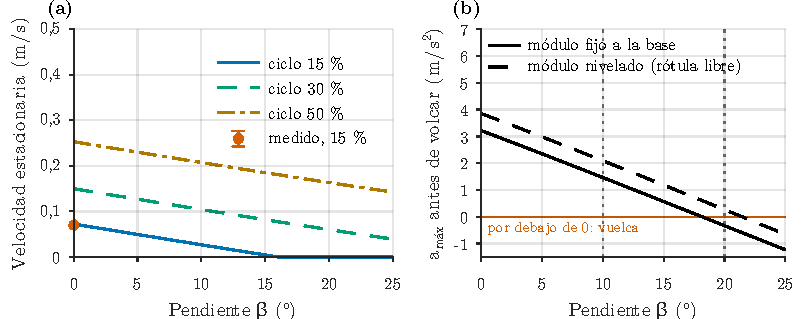
\includegraphics{figures/fig_base_limits.pdf}
  \caption{Base móvil. (a) Velocidad estacionaria frente a la pendiente según \eqref{eq:vss} para tres ciclos de trabajo y velocidad medida al 15\% en llano. (b) Margen de aceleración longitudinal antes de volcar hacia atrás \eqref{eq:tip} con el módulo en la rótula, calibrado con la pendiente de vuelco medida (punto).}
  \label{fig:base}
\end{figure}

\subsection{Dinámica del módulo aéreo}
\label{sec:aerial}

\paragraph{Modelo de rotor y asignación de control}
Cada rotor produce un empuje $F_i$ según $\vect z_D$ y un par de reacción $-c_Qs_iF_i$ alrededor de $\vect z_D$, donde $s_i=+1$ para los rotores antihorarios (vistos desde arriba). Con las posiciones de los rotores $\vect r_i=[x_i,y_i,h_r]\T$ de la Tabla~\ref{tab:params}, el empuje colectivo y los pares en ejes cuerpo son
\begin{equation}
  \begin{bmatrix}T\\ \tau_x\\ \tau_y\\ \tau_z\end{bmatrix}=\underbrace{\begin{bmatrix}\vect 1\T\\ \vect y\T\\ -\vect x\T\\ -c_Q\vect s\T\end{bmatrix}}_{\vect B\in\mathbb R^{4\times8}}\vect F,
  \qquad \vect B\vect B\T=\diag\big(8,\ 4L_r^2,\ 4L_r^2,\ 8c_Q^2\big),
  \label{eq:alloc}
\end{equation}
porque $\sum x_i=\sum y_i=\sum s_i=\sum x_iy_i=\sum s_ix_i=\sum s_iy_i=0$ y $\sum x_i^2=\sum y_i^2=4L_r^2$ para la geometría del octocóptero (la altura de los brazos $h_r$ no contribuye porque el empuje es paralelo a $\vect z_D$). Los cuatro canales son, por tanto, ortogonales y la asignación de norma mínima es explícita:
\begin{equation}
  \vect F=\vect B\T(\vect B\vect B\T)^{-1}\vect w=\frac{T}{8}\vect 1+\frac{\vect y\,\tau_x-\vect x\,\tau_y}{4L_r^2}-\frac{\vect s\,\tau_z}{8c_Q},\qquad \vect w=[T,\tau_x,\tau_y,\tau_z]\T .
  \label{eq:alloc_inv}
\end{equation}
El firmware implementa exactamente \eqref{eq:alloc_inv} \cite{johansen2013}: el colectivo fija la fuerza base $F_0=T/8$, se suman los incrementos de alabeo y cabeceo, y el incremento de guiñada se suma según la fila de guiñada proyectada en el espacio nulo de las otras tres (que, por la ortogonalidad anterior, es la propia fila de guiñada). Cuando un incremento llevaría un rotor fuera de $[F_{\min},F_{\max}]$ (\SIrange{1180}{2000}{\micro\second}), se escalan primero el alabeo y el cabeceo y después la guiñada. Para un par de cabeceo puro saturan primero los rotores del eje $x$ ($|x_i|=L_r$), de modo que el par alcanzable es
\begin{equation}
  |\tau_y|_{\max}=4L_r\,\min\{F_{\max}-F_0,\ F_0-F_{\min}\},
  \label{eq:taumax}
\end{equation}
que, con el mapa del firmware, vale \SI{3.2}{\newton\metre} con un colectivo de \SI{1750}{\micro\second} y \SI{2.4}{\newton\metre} con \SI{1816}{\micro\second}, muy por encima de los pares que pide el vuelo estacionario (Sección~\ref{sec:authority}). El firmware convierte cada fuerza en un pulso invirtiendo el mapa $F=k_F\big((u-u_0)/\SI{860}{\micro\second}\big)^n$ con $k_F=\SI{5.40}{\newton}$; si la ganancia real es $k_F'$, cada par que produce el controlador queda multiplicado por la razón de ganancias de empuje $k_T=k_F'/k_F$, que identifica la Sección~\ref{sec:ident}.

\paragraph{Ecuaciones de Newton--Euler alrededor del pivote móvil}
El conjunto que rota (masa $m$, inercia $\vect J$ respecto a la rótula, centro de masa en $\vect r_c=[\delta_x,\delta_y,h_c]\T$ en $\{D\}$) gira alrededor del centro de la rótula, un punto fijo en el cuerpo al que la base y la guía imponen la aceleración $\vect a_J$ \eqref{eq:aJ}. Para un punto fijo en un cuerpo rígido, el momento angular respecto a él es $\vect J\vect\omega_D$, y su derivada inercial es igual al momento externo menos $m\,\vect r_c\times\vect a_J$ \cite{ginsberg1998}. En componentes de $\{D\}$:
\begin{equation}
  \vect J\dot{\vect\omega}_D+\vect\omega_D\times\vect J\vect\omega_D=
  \underbrace{\sum_{i=1}^{8}\vect r_i\times F_i\ez-\sum_{i=1}^{8}c_Qs_iF_i\ez}_{[\tau_x,\ \tau_y,\ \tau_z]\T}
  +\,m\,\vect r_c\times\Rot_{WD}\T\big(\vect g_W-\vect a_J\big)-\vect\tau_f ,
  \label{eq:euler}
\end{equation}
con $\vect g_W=[0,0,-g]\T$ y $\vect\tau_f$ la fricción de la rótula. El tercer término contiene los tres acoplamientos que dominan el comportamiento del módulo. Linealizando alrededor del vuelo estacionario nivelado (verificado simbólicamente, \ref{app:derivations}):
\begin{align}
  J_x\ddot\phi&=\tau_x+m(g+a_{J,z})h_c\,\phi+m h_c\,a_{J,y}-m g\,\delta_y, \label{eq:rolllin}\\
  J_y\ddot\theta&=\tau_y+m(g+a_{J,z})h_c\,\theta-m h_c\,a_{J,x}+m g\,\delta_x, \label{eq:pitchlin}
\end{align}
con $\vect a_J$ en componentes de $\{D\}$. (i) Como $h_c>0$, el módulo es un péndulo invertido sobre la rótula, con polos en lazo abierto $\pm p$, $p=\sqrt{mgh_c/J_y}=\SI{6.1}{\radian\per\second}$ para $h_c=\SI{0.14}{\metre}$ (tiempo de duplicación \SI{0.11}{\second}). (ii) Una aceleración horizontal de la base produce el par $\mp mh_ca_J$: la parte superior del módulo se queda atrás respecto a la rótula, que es el camino principal de perturbación de la base al octocóptero. (iii) Una excentricidad horizontal $\delta$ del centro de masa produce un par constante $mg\delta$ que el controlador debe sostener de forma permanente. La aceleración vertical de la rótula modula paramétricamente la rigidez del péndulo.

A lo largo de la guía (eje $\vect z_B$), el carro y el módulo obedecen
\begin{equation}
  (m+m_c)\ddot d=T\,\vect z_D\!\cdot\!\vect z_B-(m+m_c)\big(g\cos\beta+\vect a_B\!\cdot\!\vect z_B\big)-F_g(\dot d)+F_{\mathrm{stop}},
  \label{eq:guide}
\end{equation}
de modo que el módulo despega cuando $T>(m+m_c)g\cos\beta+F_{g,\mathrm{static}}$. Mientras $T$ es menor, el módulo apoya en el tope inferior y su peso menos $T$ se transmite a la base; esta es la descarga que se aprovecha en la rampa (Sección~\ref{sec:porquedron}).

\paragraph{Potencia en vuelo estacionario}
Por la teoría de cantidad de movimiento \cite{leishman2006}, el empuje de vuelo estacionario por rotor, $T/8=\SI{4.41}{\newton}$, a través del disco de una hélice de 9,4 pulgadas induce una velocidad $v_h=\sqrt{T/(16\rho A)}=\SI{6.4}{\metre\per\second}$ y requiere una potencia ideal $Tv_h/8=\SI{28}{\watt}$ por rotor. Con una figura de mérito de 0,5 y una eficiencia motor--ESC de 0,8, los ocho rotores consumen unos \SI{570}{\watt}; la tabla del A2212 con hélice 9450, escalada a \SI{3.6}{\kilo\gram}, da \SI{500}{\watt}. Son 22--\SI{25}{\ampere} por rama con fusible, y la potencia crece como $T^{3/2}$, así que cada aumento de colectivo para compensar la caída de tensión cuesta corriente. Por eso el firmware limita a \SI{20}{\second} la operación por encima de \SI{1850}{\micro\second} (fusibles de \SI{30}{\ampere}), y por eso se mantuvo la holgura de \SI{29}{\milli\metre} entre puntas de hélice con $L_r=\SI{0.350}{\metre}$. La Sección~\ref{sec:bateria} convierte estas cifras en margen de empuje y autonomía.

\subsection{Identificación del módulo aéreo con telemetría de vuelo estacionario}
\label{sec:ident}

\paragraph{Ganancia de empuje}
En el despegue, \eqref{eq:guide} da $8k_F'\big((u-u_0)/860\big)^n=(m+m_c)g+F_{g,\mathrm{static}}$. El despegue ocurrió entre \SI{1725}{\micro\second} y \SI{1775}{\micro\second} con las LiPo cargadas, a 12,4\,V en reposo al iniciar la sesión (Sección~\ref{sec:flights}); despreciando la fricción de la guía se obtienen las cotas inferiores $k_F'=$ \SIrange{7.17}{8.18}{\newton}, de modo que la razón de ganancias de empuje es $k_T=1.33$--1,52 (Fig.~\ref{fig:ident}b). El mapa del firmware, y el modelo de Isaac Lab construido sobre él, predecían el vuelo estacionario en \SI{1899}{\micro\second}; una auditoría de potencia independiente, basada en los datos del motor y la hélice, predijo \SI{1770}{\micro\second}, dentro de la banda medida, aunque para una masa de \SI{3.10}{\kilo\gram} y no de \SI{3.6}{\kilo\gram}.

\paragraph{Centro de masa}
Durante el vuelo estacionario cuasiestático ($\dot{\vect\omega}_D\approx\vect 0$, integradores asentados, $T\approx(m+m_c)g$), \eqref{eq:rolllin}--\eqref{eq:pitchlin} se reducen a balances de momentos. Al dividir por el colectivo se elimina la ganancia desconocida $k_F'$ y queda la posición del centro de empuje,
\begin{equation}
  x_{cp}=\frac{\sum_i x_iF_i}{\sum_iF_i}=c\,(\delta_x+h_c\sin\theta),\qquad
  y_{cp}=\frac{\sum_i y_iF_i}{\sum_iF_i}=c\,(\delta_y-h_c\sin\phi),
  \label{eq:cop}
\end{equation}
con $c=m/(m+m_c)$, que es lineal en $(\delta_x,\delta_y,h_c)$ y se calcula con las órdenes de motor registradas. Promediando \eqref{eq:cop} en la fase de vuelo estacionario de los siete vuelos que despegaron (muestras con $|p|,|q|<\SI{15}{\degree\per\second}$ por encima de \SI{1650}{\micro\second}) y resolviendo las 14 ecuaciones por mínimos cuadrados se obtiene
\begin{equation}
  \hat\delta_x=9.5\pm1.8\ \mathrm{mm},\qquad \hat\delta_y=1.9\pm1.5\ \mathrm{mm},\qquad \hat h_c=0.14\pm0.06\ \mathrm{m}\quad(\pm1\sigma),
  \label{eq:idres}
\end{equation}
con un residuo de \SI{3.3}{\milli\metre} RMS (Fig.~\ref{fig:ident}a). La estimación de $h_c$ cambia menos que su incertidumbre cuando el exponente del mapa varía entre 1,3 y 1,6 (0,11--\SI{0.14}{\metre}), y es coherente con los \SI{0.10}{\metre} del modelo derivado del CAD. La excentricidad produce un par de gravedad permanente $mg\delta_x=\SI{0.31}{\newton\metre}$ hacia M8.

\begin{figure}[!htbp]
  \centering
  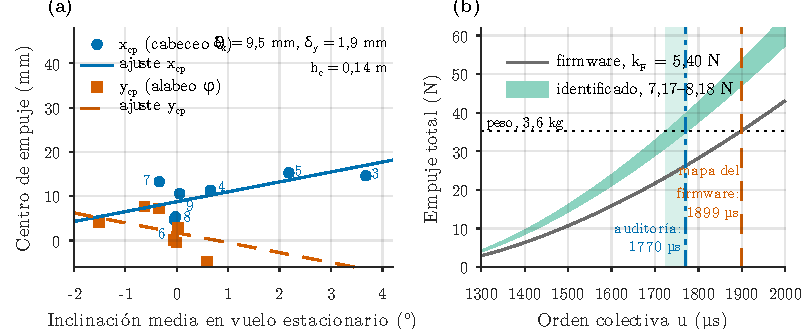
\includegraphics{figures/fig_ident.pdf}
  \caption{Identificación con telemetría de vuelo estacionario. (a) Centro de empuje frente a la inclinación media en los siete vuelos estacionarios (etiquetas: número de vuelo) y ajuste por mínimos cuadrados de \eqref{eq:cop}. (b) Empuje total del mapa del firmware, banda identificada con la condición de despegue, peso del conjunto móvil y predicciones de vuelo estacionario del mapa del firmware y de la auditoría de potencia.}
  \label{fig:ident}
\end{figure}

\subsection{Bola sobre un plato que acelera y rota}
\label{sec:ball}

Sea $\vect\Omega$ la velocidad angular del marco del plato $\{P\}$ y sea $\vect a_G$ la aceleración absoluta de su origen (el centro de la junta universal), ambas expresadas en $\{P\}$. El centro de la bola está en $\vect\rho=[x_b,y_b,\varepsilon]\T$, su velocidad angular absoluta es $\vect\omega_b$, y la rodadura sin deslizamiento (A6) exige que la velocidad del punto de contacto de la bola sea igual a la del punto del plato que toca. Esto da $\dot{\vect\rho}=r_b(\vect\omega_b-\vect\Omega)\times\ez$, es decir, la velocidad angular relativa es $\vect w=\vect\omega_b-\vect\Omega=[-\dot y_b/r_b,\ \dot x_b/r_b,\ w_z]\T$, con un giro libre $w_z$ alrededor de la normal del plato. Escribiendo la ley de Newton para el centro de la bola en el marco que rota y la ley de Euler para la bola respecto a su centro, con la fuerza de contacto aplicada en $-r_b\ez$, y eliminando las fuerzas tangenciales de contacto (\ref{app:derivations}), se obtiene, de forma exacta,
\begin{align}
  \frac{\ddot x_b}{\gamma_b}&=g_x-a_{G,x}-\kappa\dot\Omega_y+\dot\Omega_z\,y_b+(\Omega_y^2+\Omega_z^2)\,x_b-\Omega_x\Omega_y\,y_b \notag\\
   &\quad-\varepsilon\,\Omega_x\Omega_z+(2+\iota)\,\Omega_z\dot y_b+\iota r_b\,\Omega_xw_z, \label{eq:ballx}\\
  \frac{\ddot y_b}{\gamma_b}&=g_y-a_{G,y}+\kappa\dot\Omega_x-\dot\Omega_z\,x_b+(\Omega_x^2+\Omega_z^2)\,y_b-\Omega_x\Omega_y\,x_b \notag\\
   &\quad-\varepsilon\,\Omega_y\Omega_z-(2+\iota)\,\Omega_z\dot x_b+\iota r_b\,\Omega_yw_z, \label{eq:bally}\\
  \dot w_z&=-\dot\Omega_z-\frac{\Omega_x\dot x_b+\Omega_y\dot y_b}{r_b}, \label{eq:spin}
\end{align}
donde $[g_x,g_y,g_z]\T=\Rot_{WP}\T\vect g_W$ es la gravedad en $\{P\}$, $\iota=I_b/(m_br_b^2)$ ($2/5$ para una esfera maciza), $\gamma_b=1/(1+\iota)$, y
\begin{equation}
  \kappa=\varepsilon+\frac{I_b}{m_br_b}=\varepsilon+\iota r_b=\SI{42.3}{\milli\metre}
  \label{eq:kappa}
\end{equation}
es la altura efectiva de la bola sobre el eje de rotación. Las ecuaciones \eqref{eq:ballx}--\eqref{eq:spin} contienen el modelo clásico del \textit{ball and plate} como caso particular con $\vect a_G=\vect 0$, $\Omega_z=0$, $\varepsilon=0$ \cite{awtar2002,hauser1992}; los términos adicionales son la aceleración de arrastre del centro del plato, el término de Euler $\kappa\dot{\vect\Omega}$ debido a la altura de la bola, los términos centrífugo y de Coriolis de la rotación de la base y el acoplamiento del giro propio.

\paragraph{Linealización y funciones de transferencia}
Para ángulos pequeños, $g_x\simeq g\,\Theta_P$ y $g_y\simeq-g\,\Phi_P$; con \eqref{eq:tilt} y la linealización de \eqref{eq:aG}, $a_{G,x}\simeq a_{J,x}+h_P\ddot\theta$ y $a_{G,y}\simeq a_{J,y}-h_P\ddot\phi$, la bola obedece
\begin{align}
  \ddot x_b&=\gamma_b\Big[g(\theta+\alpha_y)-\kappa\,\ddot\alpha_y-(h_P+\kappa)\,\ddot\theta-a_{J,x}\Big], \label{eq:balllinx}\\
  \ddot y_b&=\gamma_b\Big[-g(\phi+\alpha_x)+\kappa\,\ddot\alpha_x+(h_P+\kappa)\,\ddot\phi-a_{J,y}\Big]. \label{eq:balllinly}
\end{align}
Las ecuaciones \eqref{eq:balllinx}--\eqref{eq:balllinly} resumen el acoplamiento de todo el robot: a la bola la mueven la inclinación de los servos (la entrada de control), la actitud residual del octocóptero amplificada por el brazo $h_P+\kappa=\SI{0.146}{\metre}$, y la aceleración de la rótula que produce la base. Con $\alpha_y=K_\alpha u$, las tres funciones de transferencia del eje $x$ son
\begin{equation}
  \frac{X_b}{U}=K_b\,\frac{1-s^2/z_1^2}{s^2},\qquad
  \frac{X_b}{\Theta}=\gamma_b g\,\frac{1-s^2/z_2^2}{s^2},\qquad
  \frac{X_b}{A_{J,x}}=-\frac{\gamma_b}{s^2},
  \label{eq:balltf}
\end{equation}
con la ganancia de planta $K_b=\gamma_bgK_\alpha=\SI{6.0}{\milli\metre\per\second\squared}$ por microsegundo (bola maciza) y los ceros $z_1=\sqrt{g/\kappa}=\SI{15.2}{\radian\per\second}$ y $z_2=\sqrt{g/(h_P+\kappa)}=\SI{8.2}{\radian\per\second}$. Cada par contiene un cero en el semiplano derecho: el camino del servo es de fase no mínima (una inclinación rápida empuja primero la bola en el sentido equivocado, porque la superficie del plato acelera bajo ella), y por encima de $z_2/2\pi=\SI{1.3}{\hertz}$ la aceleración angular del octocóptero perturba la bola más que su inclinación.

\paragraph{Rotación de la base}
Para una base que gira a velocidad constante $\omega$ ($\vect\Omega=\omega\ez$), \eqref{eq:ballx}--\eqref{eq:bally} añaden la rigidez negativa $\gamma_b\omega^2$ y el acoplamiento giroscópico $\gamma_b(2+\iota)\omega$ entre los ejes. Incluso para un giro más rápido que cualquier prueba ($\omega=\SI{0.53}{\radian\per\second}$, ruedas a $\pm\SI{0.10}{\metre\per\second}$), la rigidez negativa es \SI{0.20}{\per\second\squared}, menos del 10\% de la rigidez $K_bk_p\approx\SI{2}{\per\second\squared}$ que aporta el controlador de la bola (Sección~\ref{sec:ballcontrol}).
           % 3. Modelo: dinamica de la base, del octocoptero y de la bola
%% ======================================================================
%% 04d_dron_rampa_bateria.tex -- 3. Modelo (parte 3): por que un dron en la rampa y margen de bateria
%% Cifras: scripts_modelo/rampa.py y scripts_modelo/bateria.py
%% ======================================================================
\subsection{Por qué un dron en la rampa}
\label{sec:porquedron}

La etapa intermedia de AeroTray podría haber sido un cardán motorizado de dos ejes. Esta sección muestra qué aporta el octocóptero en la rampa y con qué costo, a partir de las ecuaciones ya deducidas.

\paragraph{Idea central: un actuador que no empuja contra la base}
Un plato movido por servos fijos a la base, o un cardán motorizado, genera su par \emph{entre} la base y el plato. Por acción y reacción ocurren tres cosas: toda inclinación de la base (la pendiente y los golpes al cruzar los quiebres de la rampa) la debe restar el mismo actuador con su recorrido; esos golpes llegan al plato a través de la transmisión rígida; y la referencia de nivel es la base. El octocóptero sobre la rótula rompe esa cadena. La rótula no transmite par, solo fuerza. El dron genera su par contra el aire y se referencia a la gravedad con su IMU. Por eso la pendiente no entra al plato, y los actuadores quedan separados por escalas: el dron se ocupa de los ángulos grandes y lentos (la pendiente, \SIrange{0}{20}{\degree}, por debajo de \SI{0.3}{\hertz}), y los servos de los ángulos pequeños y rápidos que necesita la bola. Ninguna etapa que reaccione contra la base puede ofrecer esa separación sin gastar recorrido de sus actuadores. A eso se suma una propiedad exclusiva del dron: su empuje es un lastre ajustable (punto~2).

\paragraph{Evidencia con los registros del 18/11}
En los once recorridos grabados ese día el dron iba libre en la rótula a \SI{1300}{\micro\second}. El uso medio del recorrido de los servos fue de 36--57\% en los siete recorridos de rampa y de 43--63\% en los cuatro de llano. El sesgo mediano de los pulsos en la rampa no superó \SI{\pm60}{\micro\second}. Con la bandeja fija a la base, solo nivelar la pendiente de \SI{10}{\degree} habría exigido un sesgo de unos \SI{204}{\micro\second}, es decir, el 93\% del recorrido. Los servos no trabajaron más en la rampa que en el llano: la pendiente no llegó al plato. Una prueba comparativa directa —el ensayo D descrito en la Sección~\ref{sec:metodologia}: recorrer la misma rampa con el dron trabado a la base (\emph{solo servos}) y con el dron libre para comparar uso y saturación de servos, error de la bola y pérdidas— quedó pendiente como trabajo futuro (Sección~\ref{sec:limits}).

\paragraph{1. Nivelación: la pendiente desaparece del plato}
Por \eqref{eq:tilt}, la inclinación absoluta del plato es $\theta+\alpha_y$ y no contiene $\beta$. El octocóptero lleva $\theta$ a cero con su propia IMU, así que los servos solo corrigen la posición de la bola. Con la bandeja fija a la base, la pendiente consumiría $\beta$ de los \SI{\pm10.8}{\degree} de recorrido del plato: en la rampa de \SI{10}{\degree} quedarían \SI{0.8}{\degree} para controlar la bola, y en \SI{20}{\degree} el plato no se podría nivelar. En vuelo estacionario el octocóptero mantuvo el plano de la bandeja a 0,55--1,7$^\circ$ RMS de la horizontal (Sección~\ref{sec:flights}), es decir, deja libre entre el 84 y el 95\% del recorrido de los servos. Un cardán con su propia IMU también podría nivelar, pero lo haría reaccionando contra la base y con un recorrido acotado por sus actuadores; la siguiente función, en cambio, solo la tiene el dron.

\paragraph{2. Descarga de peso: un lastre ajustable}
Sea $f=T/\big((m+m_c)g\big)\in[0,1]$ la fracción del peso del módulo que sostienen los rotores. Mientras $f<1$ el módulo apoya en el tope inferior de la guía \eqref{eq:guide}, y como se nivela, su empuje es vertical en $\{W\}$. En el balance de momentos de \eqref{eq:tip} el empuje equivale entonces a reducir la masa del módulo en la rótula a $(1-f)(m+m_c)$. Con el resto del robot (masa $M_b=\SI{6.8}{\kilo\gram}$, CM a $x_b=\SI{0.088}{\metre}$ por delante del eje motriz y $h_b=\SI{0.081}{\metre}$ sobre el apoyo, deducidos de las pendientes de vuelco medidas) y $m_a=m+m_c$,
\begin{equation}
\begin{gathered}
  M(f)=M_b+(1-f)m_a,\\
  x_G(f)=\frac{M_bx_b+(1-f)m_a\ell_J}{M(f)},\qquad
  h_G(f)=\frac{M_bh_b+(1-f)m_a(h_{J0}+d)}{M(f)},
\end{gathered}
  \label{eq:descarga}
\end{equation}
y basta sustituir \eqref{eq:descarga} en la condición estática de \eqref{eq:tip}, en \eqref{eq:vss} y en la condición de tracción de la Sección~\ref{sec:basedyn}. El margen de aceleración necesita un cuidado más: el empuje quita \emph{peso}, pero no \emph{masa}. La guía sigue acelerando los \SI{3.6}{\kilo\gram} del módulo junto con la base, así que su fuerza de d'Alembert completa actúa en la rótula y
\begin{equation}
\begin{split}
  a_{\max}(f,\beta)=\frac{g}{M_bh_b+m_a(h_{J0}+d)}\Big\{&\big[M_bx_b+(1-f)m_a\ell_J\big]\cos\beta\\
  &-\big[M_bh_b+(1-f)m_a(h_{J0}+d)\big]\sin\beta\Big\}.
\end{split}
  \label{eq:amaxf}
\end{equation} La Fig.~\ref{fig:rampa} y la Tabla~\ref{tab:rampa} muestran el resultado. El módulo de \SI{3.6}{\kilo\gram} está alto (rótula a \SI{0.5}{\metre}) y prácticamente en la misma vertical que el CM del resto del robot ($\ell_J\approx x_b\approx\SI{88}{\milli\metre}$). Por eso, sostener una fracción $f$ de su peso con los rotores no adelanta ni atrasa el CM: lo \emph{baja}, y mejora el vuelco en los dos sentidos.
\begin{itemize}
  \item \textbf{Vuelco.} Al subir, la pendiente de vuelco estático pasa de \SI{21.4}{\degree} ($f=0$; medida: \SI{21.5}{\degree}) a \SI{27.7}{\degree} ($f=0.5$) y a \SI{47.4}{\degree} ($f=1$). Al bajar, pasa de \SI{30.5}{\degree} a \SI{38.2}{\degree} y a \SI{58.5}{\degree}. En la rampa de \SI{10}{\degree}, el margen al subir crece de \SI{11.5}{\degree} a \SI{17.7}{\degree} con $f=0.5$, un 54\% más.
  \item \textbf{Margen de aceleración.} En \SI{10}{\degree} casi no cambia (\SI{2.1}{\metre\per\second\squared}), porque el empuje quita peso pero no masa \eqref{eq:amaxf}. En \SI{20}{\degree} pasa de \SI{0.26}{\metre\per\second\squared} a \SI{0.92}{\metre\per\second\squared} con $f=0.5$, es decir, se multiplica por 3,5. Es en las pendientes grandes donde la descarga se vuelve decisiva.
  \item \textbf{Tracción.} El coeficiente de fricción que necesitan las ruedas motrices sube poco: de 0,25 a 0,27 en \SI{10}{\degree} y de 0,40 a 0,44 en \SI{20}{\degree} con $f=0.5$, y a 0,52 con $f=1$. Todo queda por debajo de lo que da el caucho sobre madera (0,5--0,8). Aun así, el dron no debe flotar en la rampa: con $f=1$ la tracción en \SI{20}{\degree} queda al límite.
\end{itemize}
Proponemos una ventana de operación $f=0.35$--0,55 (\emph{modo rampa}). Corresponde a un colectivo de 1460--\SI{1560}{\micro\second} con las baterías cargadas, por debajo del umbral de vuelo del firmware (\SI{1650}{\micro\second}), y a 5--\SI{9}{\ampere} por rama (la potencia crece como $f^{3/2}$). Un minuto de subida cuesta 0,08--\SI{0.15}{\ampere\hour} por batería, un 2--5\% de su capacidad. En la rampa real del ensayo (\SI{0.7}{\metre} a \SI{10}{\degree}, \SI{0.8}{\metre} de meseta y \SI{0.7}{\metre} de bajada, \SI{12.2}{\centi\metre} de desnivel; Fig.~\ref{fig:rampa_cotas}), el modelo predice al 15\% de ciclo de trabajo un ciclo de unos \SI{41}{\second} en ralentí (subida de \SI{24}{\second}) y de \SI{37}{\second} en modo rampa (subida de \SI{20}{\second}), y unos \SI{19}{\second} al 25\% de ciclo de trabajo (ensayos del 23/11).

\begin{figure}[!htbp]
\centering
\begin{tikzpicture}[font=\footnotesize, >=Latex]
  % Escala real (1 m = 4.10 cm). Rampa medida el 24/11: 0,7 m a 10 grados + 0,8 m + 0,7 m a 10 grados
  % Q1=(0,0), Q2=(2.826, 0.498), Q3=(6.106, 0.498), Q4=(8.932, 0)
  \coordinate (Q1) at (0.000, 0.000);
  \coordinate (Q2) at (2.826, 0.498);
  \coordinate (Q3) at (6.106, 0.498);
  \coordinate (Q4) at (8.932, 0.000);

  % Suelo horizontal (aproximacion y salida)
  \fill[pGris!18] (-0.95,-0.20) rectangle (10.10,0.00);
  \draw[thick, pGris!80!black] (-0.95,0.00) -- (10.10,0.00);

  % Cuerpo de la rampa (escala 1:1)
  \fill[pGris!10] (Q1) -- (Q2) -- (Q3) -- (Q4) -- cycle;
  \draw[very thick, pGris!85!black] (Q1) -- (Q2) -- (Q3) -- (Q4);

  % Apoyos internos sutiles bajo la meseta
  \draw[dashed, pGris!60] (Q2) -- (2.826,0.00);
  \draw[dashed, pGris!60] (Q3) -- (6.106,0.00);

  % Angulos de 10 deg en Q1 y Q4
  \draw[pAzul, thick] (1.10,0.00) arc (0:10:1.10);
  \node[pAzul] at (1.52,0.11) {\SI{10}{\degree}};
  \draw[pAzul, thick] (7.832,0.00) arc (180:170:1.10);
  \node[pAzul] at (7.41,0.11) {\SI{10}{\degree}};

  % Cota vertical de altura (12,2 cm) a la derecha
  \draw[dotted, pGris] (Q3) -- (9.90,0.498);
  \draw[<->, pGris!85!black] (9.75,0.00) -- (9.75,0.498);
  \node[right=2pt, align=left] at (9.75,0.25) {\SI{12.2}{\centi\metre}};

  % Robot esquematico subiendo la rampa (proporciones reales 1:1, centrado en s=0.47 m)
  \begin{scope}[shift={(1.330,0.235)}, rotate=10]
    % Chasis base diferencial + ruedas (trocha/ejes L=0.22 m -> 0.90 cm, r=0.049 m -> 0.20 cm)
    \draw[thick, fill=pAzul!15, draw=pAzul] (-0.64,0.22) rectangle (0.64,0.52);
    \draw[thick, fill=pGris!40, draw=pGris!90!black] (-0.45,0.20) circle (0.20);
    \draw[thick, fill=pGris!12, draw=pGris!90!black] ( 0.45,0.20) circle (0.20);
    % Mastil y carro de guia vertical (l_J=0.088 m -> 0.36 cm delante del eje motriz)
    \draw[line width=1.6pt, pGris!85!black] (-0.09,0.52) -- (-0.09,1.98);
    \draw[thick, fill=pGris!25, draw=pGris!85!black] (-0.17,1.62) rectangle (-0.01,1.98);
    \coordinate (J) at (-0.09,2.03);
    \coordinate (BaseTip) at (0.64,0.40);
  \end{scope}

  % Octocoptero y bandeja nivelados (theta = 0 deg) sobre la rotula J
  \fill[black] (J) circle (0.065);
  \begin{scope}[shift={(J)}]
    % Referencia horizontal y vertical de la rotula
    \draw[dashed, pGris!70] (-1.55,0.00) -- (1.65,0.00);
    % Marco rojo del octocoptero (2 L_r = 0.70 m -> 2.87 cm)
    \draw[line width=1.4pt, pRojo] (-1.42,0.36) -- (1.42,0.36);
    \foreach \xx in {-1.42,-0.80,0.80,1.42}{
      \draw[thick] (\xx,0.36) -- (\xx,0.49);
      \draw[thick] (\xx-0.24,0.49) -- (\xx+0.24,0.49);
    }
    % Pilar, plato (ocre) y bola (azul)
    \draw[thick] (0,0.00) -- (0,0.44);
    \draw[very thick, pOcre, fill=pOcre!20] (-0.52,0.44) rectangle (0.52,0.53);
    \fill[pAzul] (0.16,0.61) circle (0.08);
    % Torres y camara cenital
    \draw[thin, pGris] (-0.92,0.36) -- (-0.12,1.20);
    \draw[thin, pGris] ( 0.92,0.36) -- ( 0.12,1.20);
    \draw[thick, fill=pGris!45] (-0.18,1.18) rectangle (0.18,1.32);
    \coordinate (OctoR) at (1.50,0.40);
  \end{scope}

  % Anotaciones limpias del robot (en el espacio libre a la derecha, sin cruzar la cota del llano)
  \draw[->, pRojo, thin] (3.65,3.20) -- (2.49,2.68);
  \node[pRojo, right, align=left] at (3.68,3.25) {octocóptero y plato\\ nivelados ($\theta\approx\SI{0}{\degree}$)};
  \draw[->, pAzul, thin] (3.72,2.15) -- (1.92,0.78);
  \node[pAzul, right, align=left] at (3.76,2.20) {base y mástil inclinados ($\beta=\SI{10}{\degree}$)};

  % Cotas paralelas a los tres tramos
  % Tramo 1: subida 0,7 m (por encima del robot, con lineas auxiliares desde Q1 y Q2)
  \coordinate (Q1u) at ($(Q1)+(-0.69,3.92)$);
  \coordinate (Q2u) at ($(Q2)+(-0.69,3.92)$);
  \draw[dotted, pGris] (Q1) -- (Q1u);
  \draw[dotted, pGris] (Q2) -- (Q2u);
  \draw[<->, thick] ($(Q1)+(-0.65,3.72)$) -- node[above=2pt, sloped]{\SI{0.7}{\metre} (subida, \SI{10}{\degree})} ($(Q2)+(-0.65,3.72)$);

  % Tramo 2: meseta 0,8 m (bajada a y=0.98 para despejar la flecha azul)
  \draw[dotted, pGris] (Q2) -- (2.826,1.12);
  \draw[dotted, pGris] (Q3) -- (6.106,1.12);
  \draw[<->, thick] (2.826,0.98) -- node[above=1.5pt]{\SI{0.8}{\metre} (llano)} (6.106,0.98);

  % Tramo 3: bajada 0,7 m
  \coordinate (Q3d) at ($(Q3)+(0.13,0.74)$);
  \coordinate (Q4d) at ($(Q4)+(0.13,0.74)$);
  \draw[dotted, pGris] (Q3) -- (Q3d);
  \draw[dotted, pGris] (Q4) -- (Q4d);
  \draw[<->, thick] ($(Q3)+(0.09,0.52)$) -- node[above=2pt, sloped]{\SI{0.7}{\metre} (bajada, \SI{10}{\degree})} ($(Q4)+(0.09,0.52)$);

  % Marcadores de los 4 quiebres de pendiente (Q1..Q4)
  \foreach \q in {Q1, Q2, Q3, Q4}{
    \fill[pRojo] (\q) circle (0.085);
  }
  \node[pRojo, font=\footnotesize\bfseries, below=4pt] at (Q1) {Q1};
  \node[pRojo, font=\footnotesize\bfseries, below left=2pt and 3pt] at (Q2) {Q2};
  \node[pRojo, font=\footnotesize\bfseries, below right=2pt and 3pt] at (Q3) {Q3};
  \node[pRojo, font=\footnotesize\bfseries, below=4pt] at (Q4) {Q4};

  % Direccion de avance y nota de quiebres debajo del suelo (separada de Q1 y Q4)
  \draw[->, thick, pGris!85!black] (-0.85,0.35) -- (-0.25,0.35);
  \node[above=1pt, pGris!85!black] at (-0.55,0.35) {avance};
  \node[pRojo] at (4.47,-0.78) {Q1--Q4: quiebres de pendiente ($0^\circ \to 10^\circ \to 0^\circ \to -10^\circ \to 0^\circ$)};
\end{tikzpicture}
\caption{Geometría de la rampa de ensayo, a escala (medida: \SI{0.7}{\metre} de subida a \SI{10}{\degree}, \SI{0.8}{\metre} de meseta y \SI{0.7}{\metre} de bajada a \SI{10}{\degree}; desnivel de \SI{12.2}{\centi\metre}, longitud horizontal de \SI{2.18}{\metre}) con AeroTray en proporción real. Los puntos Q1--Q4 señalan los cuatro quiebres donde cambia la pendiente de la base y la rótula recibe aceleraciones tangenciales $(h_{J0}+d)\ddot\theta_B$; en la subida, el octocóptero se mantiene horizontal sobre la rótula pasiva.}
\label{fig:rampa_cotas}
\end{figure}

\begin{table}[!htbp]
\centering
\caption{Efecto de la fracción de peso sostenida por los rotores, $f$, sobre la subida (modelo \eqref{eq:descarga}--\eqref{eq:amaxf} con los parámetros de la Tabla~\ref{tab:params}; $k_F'=\SI{7.6}{\newton}$, LiPo cargadas). En ralentí (\SI{1300}{\micro\second}) los rotores ya sostienen el 12\% del peso.}
\label{tab:rampa}
\resizebox{\textwidth}{!}{%
\begin{tabular}{@{}lccccccc@{}}
\toprule
$f$ & Vuelco subiendo & Vuelco bajando & $a_{\max}$ en 20° & $\mu$ req.\ 10° & $\mu$ req.\ 20° & Colectivo & $I$ por rama \\
 & (°) & (°) & (\si{\metre\per\second\squared}) & & & (\si{\micro\second}) & (\si{\ampere}) \\
\midrule
0 (motores parados) & 21,4 (medido 21,5) & 30,5 (medido 30,5) & 0,26 & 0,25 & 0,40 & $\le$1140 & 0 \\
0,12 (ralentí) & 22,5 & 31,9 & 0,42 & 0,25 & 0,40 & 1300 & 0,9 \\
0,25 & 23,9 & 33,6 & 0,59 & 0,26 & 0,41 & 1397 & 2,8 \\
0,50 & 27,7 & 38,2 & 0,92 & 0,27 & 0,44 & 1537 & 7,9 \\
0,75 & 34,2 & 45,6 & 1,25 & 0,28 & 0,47 & 1652 & 14,5 \\
1 & 47,4 & 58,5 & 1,57 & 0,30 & 0,52 & 1752 & 22,3 \\
\bottomrule
\end{tabular}}
\end{table}

\begin{figure}[!htbp]
  \centering
  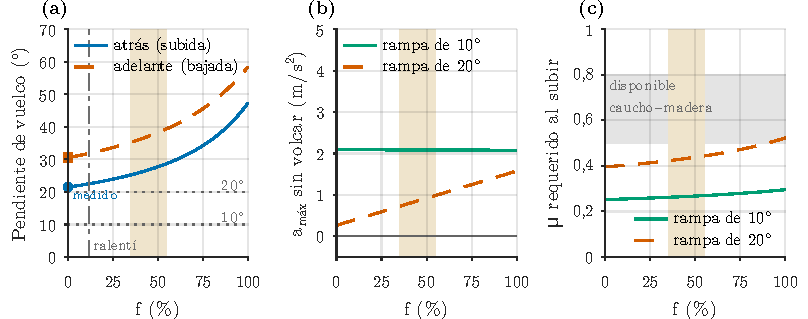
\includegraphics{figures/fig_rampa.pdf}
  \caption{Descarga de peso en la rampa frente a la fracción del peso del módulo sostenida por los rotores, $f$ ($f=0.5$ equivale a unos \SI{1540}{\micro\second} de colectivo). (a) Pendiente de vuelco estático hacia atrás (subida de frente) y hacia adelante (bajada de frente); los puntos son las pendientes medidas el 23/11 con el módulo trabado. (b) Margen de aceleración sin vuelco en 10 y \SI{20}{\degree}, con la inercia completa del módulo \eqref{eq:amaxf}. (c) Coeficiente de fricción que necesitan las ruedas motrices al subir, con la banda de caucho sobre madera. La franja ocre es la ventana propuesta de modo rampa.}
  \label{fig:rampa}
\end{figure}

\paragraph{3. Balance frente a un cardán}
La comparación honesta con un cardán ligero es la siguiente. Un cardán motorizado de \SI{1}{\kilo\gram} a la misma altura daría, con el mismo modelo, \SI{33.3}{\degree} de vuelco al subir sin gastar energía; el octocóptero solo lo supera con $f>0.72$. La ventaja del dron no es, por tanto, su masa, sino que su lastre es \emph{ajustable}: con $f=0$ carga las ruedas motrices para la tracción, con $f\approx0.5$ equilibra vuelco y tracción, y con $f=1$ desaparece de la base. Un cardán es un lastre fijo. A esto se suma que el octocóptero es el objeto de estudio del proyecto: un péndulo invertido con retardo de actuadores y autoridad de par limitada que se valida aquí, cautivo y con registros, antes del vuelo libre. El costo es doble: energía (Sección~\ref{sec:bateria}) y una banda de 0,2--\SI{0.3}{\hertz} en la que el octocóptero amplifica las aceleraciones de la base (Sección~\ref{sec:coupling}), que las rampas de referencia de la base deben evitar.

\paragraph{Lo que se ensayó y lo que falta}
Los recorridos por la rampa de \SI{10}{\degree} del 18/11 se hicieron con el firmware de banco y el colectivo en \SI{1300}{\micro\second} ($f\approx0.12$): el dron niveló la bandeja y descargó muy poco peso. La descarga es, por ahora, una predicción del modelo. Su validación necesita tres medidas: la corriente de la base con pinza amperimétrica, el ciclo de trabajo necesario para subir a velocidad constante con $f=0$ y $f=0.5$, y el ángulo al que la base empieza a levantar las ruedas omnidireccionales en una rampa variable.

\subsection{Margen de empuje y autonomía frente a la batería}
\label{sec:bateria}

El 20/11 el módulo despegó con las LiPo a 12,4\,V en reposo y, más tarde, con 11,1\,V ya no despegó. Esta sección explica el hecho y calcula el margen y la autonomía.

\paragraph{Modelo}
Cada ESC aplica al motor una fracción de la tensión de su rama, $V_{\mathrm{bus}}$. Con la hélice como carga, la velocidad del rotor es proporcional a esa tensión y el empuje a su cuadrado, así que, a orden fija,
\begin{equation}
  T=8k_F'\Big(\frac{V_{\mathrm{bus}}}{V_{\mathrm{ref}}}\Big)^2\Big(\frac{u-u_0}{860}\Big)^n ,
  \label{eq:tv}
\end{equation}
donde $k_F'$ es la ganancia identificada con la tensión $V_{\mathrm{ref}}$ de la Sección~\ref{sec:ident}. La tensión de la rama es la tensión en vacío de la LiPo, $V_{oc}$, menos la caída en la resistencia interna, el cable de \SI{1}{\metre} y los contactos (fusible, relé, XT60), $R_\Sigma$. Como la potencia de vuelo estacionario $P_b$ por rama es fija (el empuje es el peso), la corriente es $I_b=P_b/V_{\mathrm{bus}}$, y
\begin{equation}
  V_{\mathrm{bus}}=\tfrac12\Big(V_{oc}+\sqrt{V_{oc}^2-4R_\Sigma P_b}\Big).
  \label{eq:vbus}
\end{equation}
Igualando \eqref{eq:tv} al peso, el colectivo de despegue a otra tensión es
\begin{equation}
  u_{\mathrm{req}}=u_0+860\,x_{\mathrm{ref}}\Big(\frac{V_{\mathrm{bus,ref}}}{V_{\mathrm{bus}}}\Big)^{2/n},\qquad x_{\mathrm{ref}}=\frac{u_{\mathrm{ref}}-u_0}{860}=0.68\text{--}0{,}74,
  \label{eq:ureq}
\end{equation}
y con $n=1.6$ el colectivo crece con la potencia $1{,}25$ de la caída relativa de tensión. Los datos de entrada son: $P_b=\SI{250}{\watt}$ (tabla del A2212 con hélice 9450 de la auditoría, \SI{4.2}{\ampere} a 370\,gf con 11,1\,V, escalada con $T^{3/2}$ a 441\,gf por motor); $R_\Sigma=3r_c+\SI{22.6}{\milli\ohm}$, con $r_c=6$--\SI{15}{\milli\ohm} por celda [E] y un aumento del 50\% por debajo del 40\% de carga; y la curva típica tensión en reposo--estado de carga de una celda LiPo [E]. Las bandas de los resultados combinan los extremos de $k_F'$ y de $r_c$.

\paragraph{Resultados}
La Fig.~\ref{fig:bateria} y la Tabla~\ref{tab:bateria} dan el colectivo de despegue y la relación empuje/peso disponible frente a la tensión en reposo:
\begin{itemize}
  \item Con 12,4\,V (93\% de carga) la rama entrega \SI{22}{\ampere} a \SI{11.2}{\volt}. El módulo despega a 1725--\SI{1775}{\micro\second}: la orden \texttt{flotar} del firmware (\SI{1750}{\micro\second}) cae justo en esa banda. En el límite sostenido de \SI{1850}{\micro\second} la relación empuje/peso es 1,20--1,36, y en el máximo de \SI{1950}{\micro\second}, 1,48--1,68.
  \item Con 11,1\,V en reposo (12\% de carga) la tensión de la rama cae a \SI{9.3}{\volt} con \SI{27}{\ampere}, y el despegue exige 1850--\SI{2000}{\micro\second}: en el mejor caso, justo el límite sostenido, sin margen para el control de actitud; en el peor, más de lo que el ESC puede dar. Esto coincide con lo observado.
  \item La tensión mínima en reposo para despegar sin pasar de \SI{1850}{\micro\second} es 11,1--\SI{11.6}{\volt} (12--60\% de carga). Con la orden fija \texttt{flotar}, el módulo solo despega por encima de 12,05--\SI{12.1}{\volt}, y en el extremo pesimista de $k_F'$ no despega nunca.
  \item \textbf{Autonomía.} Desde 12,4\,V, el vuelo estacionario continuo dura 2,7--\SI{6.8}{\minute} hasta que el despegue exige \SI{1850}{\micro\second} (3,3--\SI{7.4}{\minute} desde 12,6\,V). El límite por energía con 80\% de descarga sería \SI{6.6}{\minute}. Lo que limita el vuelo es, por tanto, el margen de empuje y no la capacidad: solo se aprovecha la parte alta de la curva de descarga.
\end{itemize}

\begin{table}[!htbp]
\centering
\caption{Margen de empuje frente a la tensión en reposo de las LiPo (modelo \eqref{eq:vbus}--\eqref{eq:ureq}). Colectivo central con $u_{\mathrm{ref}}=\SI{1750}{\micro\second}$ y $r_c=\SI{10}{\milli\ohm}$; entre paréntesis, la banda.}
\label{tab:bateria}
\footnotesize
\setlength{\tabcolsep}{4pt}
\begin{tabular}{@{}cccccc@{}}
\toprule
$V_{oc}$ (V) & Carga (\%) & $V_{\mathrm{bus}}$ (V) & $I_b$ (A) & $u_{\mathrm{req}}$ (\si{\micro\second}) & Empuje/peso a \SI{1850}{\micro\second} \\
\midrule
12,6 & 100 & 11,45 & 21,8 & 1735 (1710--1760) & 1,24--1,42 \\
12,4 & 93 & 11,23 & 22,3 & 1750 (1725--1775) & 1,20--1,36 \\
12,2 & 84 & 11,00 & 22,7 & 1766 (1739--1793) & 1,14--1,31 \\
12,0 & 78 & 10,78 & 23,2 & 1782 (1754--1811) & 1,09--1,26 \\
11,8 & 68 & 10,55 & 23,7 & 1799 (1769--1831) & 1,04--1,21 \\
11,6 & 59 & 10,33 & 24,2 & 1817 (1786--1852) & 1,00--1,16 \\
11,4 & 40 & 10,10 & 24,8 & 1837 (1803--1875) & 0,95--1,12 \\
11,1 & 12 & 9,32 & 26,8 & 1910 (1850--2000) & 0,74--1,00 \\
\bottomrule
\end{tabular}
\end{table}

\begin{figure}[!htbp]
  \centering
  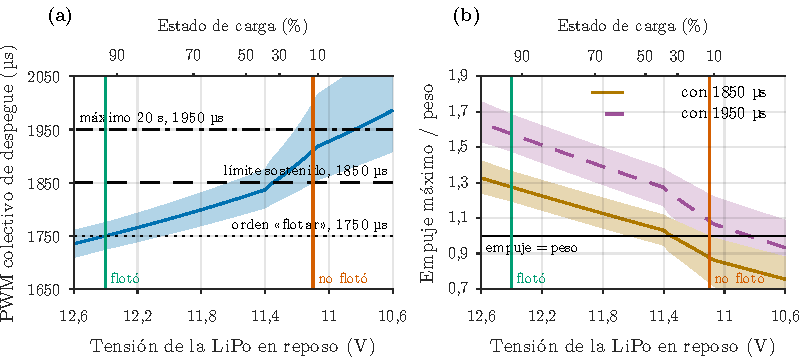
\includegraphics{figures/fig_bateria.pdf}
  \caption{Margen de empuje frente a la tensión en reposo de las LiPo. (a) Colectivo de despegue \eqref{eq:ureq}: línea central y banda por la incertidumbre de $k_F'$ y de la resistencia interna; líneas horizontales: orden \texttt{flotar}, límite sostenido y máximo del firmware v11; eje superior: estado de carga. (b) Relación empuje/peso disponible en el límite sostenido y en el máximo.}
  \label{fig:bateria}
\end{figure}

\paragraph{Contraste con los registros}
La carga que sacó cada batería en los vuelos 6--9 del 20/11, integrada a partir de las órdenes de motor registradas con el mismo modelo de potencia, fue 0,10, 0,22, 0,25 y \SI{0.44}{\ampere\hour} (\SI{1.0}{\ampere\hour}, el 31\% de la capacidad). Con ella, \eqref{eq:ureq} predice que el despegue del vuelo 9 necesitaba \SI{1787}{\micro\second} (banda 1758--\SI{1817}{\micro\second}); el registro muestra el despegue a \SI{1796}{\micro\second}, frente a \SI{1775}{\micro\second} en el vuelo 8. Al terminar el vuelo 9 el modelo da unos 11,6\,V en reposo, justo en el borde del límite sostenido. La lectura de 11,1\,V corresponde a una descarga mayor que la registrada: intentos posteriores sin registro o una medición hecha bajo carga o poco después de aterrizar, cuando la LiPo aún no se ha recuperado. Por eso el procedimiento de operación (Sección~\ref{sec:operation}) pide medir en reposo y registrar la tensión.

\paragraph{Consecuencias de diseño}
(i) El firmware debe leer VBAT\_A y VBAT\_B (los divisores ya están cableados en GPIO34/35; la auditoría recomienda pasar R2 y R4 a \SI{2.2}{\kilo\ohm} para quedar en la zona lineal del ADC, por debajo de \SI{2.45}{\volt}) y compensar el colectivo con \eqref{eq:ureq} como prealimentación, de modo que \texttt{flotar} signifique empuje igual al peso y no un pulso fijo. (ii) Conviene abortar la sesión cuando el despegue pida más de \SI{1825}{\micro\second}, para conservar margen de par. (iii) Las cuatro LiPo del grupo permiten dos sesiones de 3--\SI{7}{\minute} de vuelo continuo; el modo rampa de la Sección~\ref{sec:porquedron} cuesta mucho menos (2--5\% de carga por minuto) y es compatible con esa autonomía. (iv) Un cable de 12\,AWG reduce la caída del cable de \SI{0.34}{\volt} a unos \SI{0.2}{\volt}, lo que equivale a unos \SI{10}{\micro\second} de colectivo.
 % 3. Modelo: por que un dron en la rampa; margen de bateria
%% ======================================================================
%% 04c_coupling_control.tex -- 3. Modelo (parte 4): controladores, modelo acoplado, propagacion
%% de perturbaciones y limitaciones fundamentales
%% ======================================================================
\subsection{Controladores y análisis en lazo cerrado}
\label{sec:control}

La Fig.~\ref{fig:loops} muestra los tres lazos y los acoplamientos físicos entre ellos. Cada lazo corre en su propio procesador y solo ve a los demás a través de la mecánica.

\begin{figure}[!htbp]
\centering
\begin{tikzpicture}[font=\footnotesize, >=Latex,
  blk/.style={draw, rounded corners=2pt, align=center, minimum height=10mm, inner xsep=3pt, inner ysep=2.5pt, line width=0.6pt, fill=#1},
  blk/.default=white]
  % lazo de la base (x: 0.00..5.62)
  \node[blk=pAzul!10, draw=pAzul, text width=2.48cm] (bc) at (1.35, 0.00) {myRIO\\ PI por rueda\\ + ir a un punto};
  \node[blk=pAzul!10, draw=pAzul, text width=1.88cm] (bp) at (4.62, 0.00) {base\\ \eqref{eq:basev}--\eqref{eq:motor}};
  \draw[->, line width=0.7pt] (bc) -- node[above=1.5pt]{$u_{R,L}$} (bp);
  \draw[->, line width=0.7pt] (bp.south) -- ++(0,-0.65) -| node[pos=0.25, below=1.5pt]{encoders, odometría \eqref{eq:odo}} (bc.south);

  % lazo del dron
  \node[blk=pVerde!10, draw=pVerde, text width=2.48cm] (dc) at (1.35, 3.15) {ESP32\\ P-I-D de ángulo $\to$\\ PI de velocidad\\ $\to$ \eqref{eq:alloc_inv}};
  \node[blk=pVerde!10, draw=pVerde, text width=1.88cm] (dp) at (4.62, 3.15) {octocóptero\\ en la rótula\\ \eqref{eq:pitchlin}};
  \draw[->, line width=0.7pt] (dc) -- node[above=1.5pt]{$\vect F$} (dp);
  \draw[->, line width=0.7pt] (dp.north) -- ++(0,0.72) -| node[pos=0.25, above=1.5pt]{IMU (filtro compl.)} (dc.north);

  % lazo de la bola (x: 9.05..13.70)
  \node[blk=pOcre!12, draw=pOcre, text width=1.98cm] (cc) at (10.12, 3.15) {ESP32-S3\\ PID sobre\\ $(x_b,y_b)$};
  \node[blk=pOcre!12, draw=pOcre, text width=1.98cm] (bb) at (10.12, 0.00) {bola en el\\ plato \eqref{eq:balllinx}};
  \node[blk=pGris!10, draw=pGris, text width=2.02cm] (cam) at (12.50, 1.58) {cámara 187 fps\\ + Pi\\ (velocidad MC)};
  \draw[->, line width=0.7pt] (cc) -- node[left=2pt, align=right]{$u$ (servos,\\ mecanismo)} (bb);
  \draw[->, line width=0.7pt] (bb.east) -| (cam.south);
  \draw[->, line width=0.7pt] (cam.north) |- (cc.east);

  % acoplamientos fisicos (rojo #D55E00)
  \draw[->, line width=1.15pt, pRojo] (bp.east) -- node[below=2.5pt, align=center]{aceleración de la\\ rótula $\vect a_J$ \eqref{eq:aJ}} (bb.west);
  \draw[->, line width=1.15pt, pRojo] (bp.north) -- node[left=2pt, align=right]{$-mh_c\vect a_J$} (dp.south);
  \draw[->, line width=1.15pt, pRojo] (dp.east) -- node[above=3pt, align=center]{inclinación $\theta,\phi$ y $\ddot\theta,\ddot\phi$\\ (brazo $h_P+\kappa$)} (cc.west);
  \node[pRojo, align=center] at (6.72, 1.58) {acoplamientos\\ físicos};

  % perturbacion directa sobre la bola (sin cruzar ningun lazo)
  \node[align=center] (dist) at (11.15, -1.20) {flujo de aire, vibración $d_b$};
  \draw[->, dashed, line width=0.7pt] (dist.north -| bb.south) -- (bb.south);
\end{tikzpicture}
\caption{Los tres lazos de control de AeroTray y sus acoplamientos físicos (flechas gruesas). El controlador del octocóptero regula su actitud respecto a la gravedad; el controlador de la bola inclina el plato respecto al octocóptero; la cámara está fija al octocóptero.}
\label{fig:loops}
\end{figure}

\subsubsection{Actitud del octocóptero}
\label{sec:attitude}

\paragraph{Estimador y ley de control}
La actitud se estima a \SI{200}{\hertz} integrando las derivadas de los ángulos de Euler \eqref{eq:euler_rates} a partir del giróscopo con el sesgo corregido, y corrigiéndolas hacia la inclinación del acelerómetro con un filtro complementario \cite{mahony2008}. El acelerómetro se filtra antes con un pasabajos de \SI{10}{\hertz}, la constante de tiempo de la corrección es \SI{1}{\second} por encima de \SI{1400}{\micro\second} (\SI{0.25}{\second} por debajo), y la corrección se omite cuando la fuerza específica filtrada se aleja de $1\,g$ en más de 0,15\,g, porque la vibración de los rotores llegó a 2\,g. El controlador es una cascada \cite{mahony2012,pounds2010}; para el eje de cabeceo,
\begin{align}
  \dot\theta_{\mathrm{ref}}&=\sat_{\omega_{\lim}}\!\Big(-k_{p\theta}\,\theta-k_{d\theta}\,\dot\theta_f+k_{i\theta}\!\int\!(-\theta)\,\dd t\Big), \notag\\
  \tau_y&=k_{p\omega}(q_{\mathrm{ref}}-q)+k_{i\omega}\!\int\!(q_{\mathrm{ref}}-q)\,\dd t, \label{eq:cascade}
\end{align}
donde $\dot\theta_f$ es la derivada del ángulo de Euler filtrada con una constante de tiempo de \SI{25}{\milli\second}, $q_{\mathrm{ref}}$ se obtiene de $(\dot\phi_{\mathrm{ref}},\dot\theta_{\mathrm{ref}})$ invirtiendo \eqref{eq:euler_rates}, y los pares se asignan con \eqref{eq:alloc_inv}. Las ganancias son $k_{p\theta}=\SI{4.62}{\per\second}$, $k_{d\theta}=0.12$, $k_{p\omega}=\SI{0.848}{\newton\metre\second\per\radian}$, $k_{i\omega}=\SI{0.10}{\newton\metre\per\radian}$, y $k_{i\theta}=0.8$ en banco y $2.0$ en vuelo. La velocidad angular pedida se limita a $\omega_{\lim}=\SI{25}{\degree\per\second}$ en banco y \SI{60}{\degree\per\second} en vuelo, y la integral de velocidad a \SI{0.3}{\radian} y \SI{3.0}{\radian}, respectivamente. El lazo de guiñada vuelve lentamente al rumbo inicial ($\pm\SI{15}{\degree\per\second}$, $|\tau_z|\le\SI{0.06}{\newton\metre}$).

\paragraph{Estabilidad lineal}
Al cerrar \eqref{eq:pitchlin} con \eqref{eq:cascade}, la razón de ganancias de empuje $k_T$, el retraso del motor $\tau_m$ y el retardo de actuación $T_a$ (Tabla~\ref{tab:params}), el lazo interno $k_Tk_{p\omega}/(J_ys)$ cruza a \SI{10}{\radian\per\second} con \SI{43}{\degree} de margen de fase para $k_T=1.42$. El lazo externo debe vencer la rigidez negativa del péndulo invertido. Despreciando los integradores lentos y el actuador rápido, el lazo cerrado es $J_y\ddot\theta+c\dot\theta+(k_Tk_{p\omega}k_{p\theta}-mgh_c)\theta=0$, que solo es estable si
\begin{equation}
  k_T\,k_{p\omega}\,k_{p\theta}>m\,g\,h_c .
  \label{eq:stiff}
\end{equation}
La Fig.~\ref{fig:dronestab}b muestra la región de estabilidad del modelo lineal completo (cascada, integradores, filtro derivativo, retraso del motor y una aproximación de Pad\'e de segundo orden de $T_a$) en el plano $(h_c,k_T)$; su frontera está solo 6--12\% por encima de \eqref{eq:stiff} y es casi insensible a cambios de $\pm25\%$ en $J_y$. Con los valores identificados el margen es pequeño: $k_Tk_{p\omega}k_{p\theta}=\SI{5.6}{\newton\metre\per\radian}$ frente a $mgh_c=\SI{4.5}{\newton\metre\per\radian}$. De ahí se siguen dos consecuencias. Primero, si el mapa de empuje del firmware hubiera sido exacto ($k_T=1$), el lazo sería inestable para $h_c>\SI{0.11}{\metre}$; el controlador funcionó porque la ganancia real de empuje es mayor que la supuesta. Como $k_T$ escala con $V_{\mathrm{bus}}^2$ \eqref{eq:tv}, la misma condición explica que al descargarse la batería el margen de rigidez se reduzca: con 11,6\,V en reposo $k_T$ cae un 15\% y \eqref{eq:stiff} queda prácticamente en el límite. Segundo, la rigidez neta pequeña, combinada con la integral de ángulo, produce un modo lento y poco amortiguado en lazo cerrado: $\zeta=0.24$ a \SI{0.30}{\hertz} con las ganancias de vuelo y $\zeta=0.42$ a \SI{0.20}{\hertz} con la ganancia integral de banco. Los espectros de actitud de los vuelos estacionarios tienen su pico en 0,15--\SI{0.23}{\hertz} (periodos de 4--7\,s), de acuerdo con este modo.

\paragraph{Autoridad de par y región de atracción}
\label{sec:authority}
Cuando la velocidad angular pedida satura, el par restaurador cuasiestático no puede superar
\begin{equation}
  \tau_{\mathrm{avail}}=k_T\big(k_{p\omega}\,\omega_{\lim}+k_{i\omega}\,I_{\lim}\big),
  \label{eq:tauavail}
\end{equation}
mientras que sostener una inclinación $\theta$ requiere $mg(\delta_x+h_c\sin\theta)$ por \eqref{eq:pitchlin}. La recuperación es imposible más allá de
\begin{equation}
  \theta^\ast=\arcsin\!\Big(\frac{\tau_{\mathrm{avail}}/(mg)-\delta_x}{h_c}\Big).
  \label{eq:thetastar}
\end{equation}
Con los límites de banco de los firmware v4--v7, $\tau_{\mathrm{avail}}=0.40k_T=$ 0,53--\SI{0.61}{\newton\metre} y $\theta^\ast=$ 2,8--\SI{3.8}{\degree} para el $h_c$ identificado (2,0--\SI{6.7}{\degree} en todo su intervalo de incertidumbre): ningún transitorio de despegue mayor que unos pocos grados podía recuperarse, y el módulo derivaba lentamente hasta el enclavamiento de \SI{12}{\degree}, como se observó en los vuelos 3--6 (Fig.~\ref{fig:dronestab}a). Los límites de vuelo de v8--v9 elevan $\tau_{\mathrm{avail}}$ a 1,6--\SI{1.8}{\newton\metre} y $\theta^\ast$ a 16--\SI{19}{\degree}, más allá del enclavamiento; los dos vuelos siguientes se mantuvieron en el aire. El cambio decisivo fue, por tanto, el límite de la velocidad angular pedida y no las ganancias, lo que concuerda con el comportamiento idéntico de v5 (ganancias completas) y v6 (75\% de las ganancias). Ninguno de los dos límites lo imponen los motores: por \eqref{eq:taumax} la asignación puede entregar más de \SI{2.4}{\newton\metre} por debajo de \SI{1816}{\micro\second}.

\begin{figure}[!htbp]
  \centering
  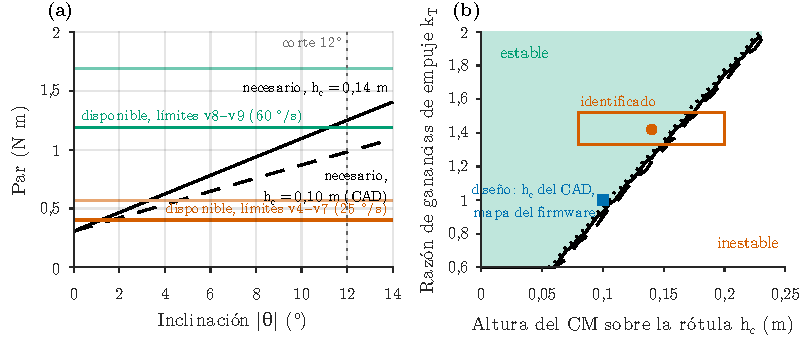
\includegraphics{figures/fig_drone_stability.pdf}
  \caption{Lazo de actitud del octocóptero. (a) Par de gravedad necesario para sostener una inclinación (valores identificado y CAD de $h_c$) y par disponible cuando satura la velocidad angular pedida \eqref{eq:tauavail}, con los límites de banco y de vuelo; líneas gruesas $k_T=1$, líneas finas $k_T=1.42$. (b) Región de estabilidad del modelo lineal completo en el plano $(h_c,k_T)$; la frontera se dibuja para $J=0.12$ (continua), 0,09 (trazos) y \SI{0.15}{\kilo\gram\metre\squared} (puntos). El rectángulo es la incertidumbre identificada y el cuadrado, el punto de diseño ($h_c$ del CAD, mapa del firmware).}
  \label{fig:dronestab}
\end{figure}

\subsubsection{\textit{Ball and plate}}
\label{sec:ballcontrol}

\paragraph{Ley de control}
La ESP32-S3 calcula, para cada eje y para cada cuadro de cámara recibido,
\begin{equation}
  u=u_n+\sat_{\pm220}\Big(k_p\,e+k_i\!\int\!e\,\dd t-k_d\,\hat v\Big),\qquad e=-x_b,
  \label{eq:ballpid}
\end{equation}
con la velocidad $\hat v$ de \eqref{eq:lsvel} que calcula la Pi. El firmware trabaja en unidades de \SI{3}{\milli\metre}; en unidades coherentes con el SI, las ganancias $(1.5;\ 0.8;\ 4.5)$ pasan a $k_p=\SI{0.50}{\micro\second\per\milli\metre}$, $k_i=\SI{0.27}{\micro\second\per\milli\metre\per\second}$ y $k_d=\SI{1.5}{\micro\second\per\milli\metre\second}$. Los pulsos neutros son $u_n=(1386;\ 1392)$\,µs, la integral se limita al 90\% del rango de salida y el juego de la Sección~\ref{sec:linkage} se suma con una rampa de \SI{30}{\micro\second}.

\paragraph{Análisis de estabilidad en tiempo discreto}
Como la derivada actúa a través de un filtro FIR y el lazo contiene varios retardos puros (exposición y transferencia del cuadro, procesamiento, la trama de \SI{50}{\hertz} del servo y el tiempo muerto del servo analógico), el lazo se analizó en tiempo discreto con el periodo de la cámara $h$: la planta \eqref{eq:balltf} con un retraso del servo $\tau_s=\SI{50}{\milli\second}$ se discretizó con retenedor de orden cero, el retardo total $T$ se representó con $T/h$ retardos unitarios, la derivada con el FIR exacto \eqref{eq:lsvel} y la integral con Euler hacia adelante, y la estabilidad se decidió con las raíces del polinomio característico en lazo cerrado. La Fig.~\ref{fig:ballstab}a muestra el mayor $k_d$ estable (en unidades del firmware) en función de $T$ para varias ganancias de planta. Con la ganancia del CAD, $K_b=6.0$, el $k_d=4.5$ nominal solo es estable si $T\lesssim\SI{40}{\milli\second}$, menos que la suma de los retardos del cuadro, del procesamiento, de la trama del servo de \SI{50}{\hertz} y del tiempo muerto del servo. En banco, $k_d=4.5$ fue estable y $k_d=6$ inestable con los rotores apagados; para retardos plausibles ($T=$ 60--\SI{180}{\milli\second}) el modelo reproduce ambas observaciones solo con una ganancia efectiva $K_{b,\mathrm{eff}}=3.5$--4,9 (58--82\% del valor del CAD), donde las ganancias más altas corresponden a los retardos más cortos. La reducción es coherente con el juego del mecanismo, cuya función descriptiva baja la ganancia de pequeña señal, y con una regresión directa de la aceleración de la bola sobre los pulsos de servo registrados, que da 2,5 y 4,9 para los ejes $x$ e $y$ ($R^2=0.29$ y 0,45, limitada por el registro de los pulsos a 20\,Hz). Para $K_{b,\mathrm{eff}}=4.2$ y $T=\SI{0.10}{\second}$ el lazo cerrado tiene un modo rápido poco amortiguado a \SI{1.3}{\hertz} ($\zeta=0.06$), la firma de operar cerca del límite por retardo, y un modo integral lento a \SI{0.064}{\hertz} ($\zeta=0.37$, periodo de \SI{16}{\second}).

\begin{figure}[!htbp]
  \centering
  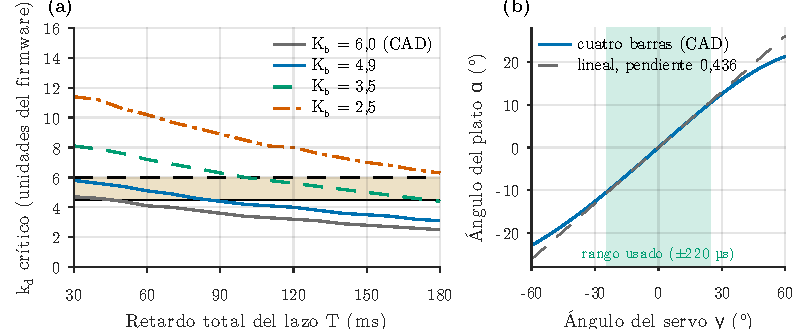
\includegraphics{figures/fig_ball_stability.pdf}
  \caption{\textit{Ball and plate}. (a) Mayor ganancia derivativa estable (unidades del firmware, $k_p=1.5$, $k_i=0.8$) frente al retardo total del lazo para cuatro ganancias de planta; la banda sombreada está acotada por la ganancia que fue estable en banco ($k_d=4.5$, línea continua) y la que no lo fue ($k_d=6$, trazos). (b) Ángulo del plato frente al ángulo del servo según la solución cerrada del cuatro barras \eqref{eq:freud} y su linealización.}
  \label{fig:ballstab}
\end{figure}

\subsubsection{Base móvil}
\label{sec:basecontrol}
Cada rueda tiene un lazo PI de velocidad con integración condicional (la integral se congela cuando la salida satura en 0 o 100\% de ciclo de trabajo), con PWM de \SI{1}{\kilo\hertz}. El modo de ir a un punto usa el error polar $\rho=\|\vect p_g-\vect p\|$, $e_\psi=\operatorname{atan2}(\Delta y,\Delta x)-\psi$, cuya cinemática se sigue de \eqref{eq:diff}: $\dot\rho=-v\cos e_\psi$, $\dot e_\psi=-\omega+(v/\rho)\sin e_\psi$. La ley es $\omega=\sat_{0.2}(1.2e_\psi)$, con $v=0$ mientras $|e_\psi|>\SI{0.2}{\radian}$ y $v=\min\{0.05;\ \max(0.025;\ 0.8\rho)\}$\,m/s en otro caso, y se detiene cuando $\rho<\SI{2}{\centi\metre}$. Como ninguna realimentación suave e invariante en el tiempo puede estabilizar la pose completa de un uniciclo \cite{brockett1983}, la ley solo regula la posición; su convergencia se sigue de cotas elementales. En la fase de giro, $|e_\psi|$ disminuye a no menos de \SI{0.2}{\radian\per\second} hasta que $|e_\psi|\le0.2$. En la fase de avance, $\dot\rho\le-0.025\cos0.2<0$, y $V=e_\psi^2/2$ cumple $\dot V\le-(\omega/e_\psi-v/\rho)\,e_\psi^2$ con $\omega/e_\psi\ge1$ y $v/\rho\le0.8$ para $\rho\ge\SI{3.1}{\centi\metre}$, de modo que $|e_\psi|$ no crece y el robot alcanza la tolerancia en tiempo finito tras a lo sumo una fase de giro.

\subsubsection{Altura y rumbo del octocóptero (firmware v11)}
\label{sec:altura}
\paragraph{Rumbo sobre la base} El octocóptero funciona de forma independiente: no recibe datos de la base. En ralentí ($\le\SI{1400}{\micro\second}$), mientras va montado sobre la base, mantiene el rumbo con que arrancó, pero con una \emph{ventana deslizante} de $\pm\SI{20}{\degree}$. Si un giro de la base lo arrastra más allá, la referencia se desliza con él en lugar de cortar los motores. Así no pelea contra la rótula en un giro de \SI{360}{\degree}, y al detenerse la base queda quieto con un desfase de \SI{20}{\degree} como máximo. Queda un corte de seguridad a \SI{120}{\degree\per\second}. Por encima de \SI{1400}{\micro\second} se conserva el comportamiento de v9: mantener el rumbo con cortes a \SI{20}{\degree} y \SI{35}{\degree\per\second}. Con el v9, los giros de la base terminaban en el corte de \SI{20}{\degree}.

\paragraph{Medición de altura} El VL53L0X no dio ninguna medida válida en los vuelos del 20/11. El \SI{80}{\percent} de las lecturas tuvo el código 2 (\emph{signal fail}): la señal de retorno desde el piso del laboratorio (0,06--\SI{0.3}{MCPS}) quedaba por debajo de la luz ambiente infrarroja (0,7--\SI{0.99}{MCPS}). Se aplicaron cuatro medidas:
\begin{enumerate}[label=(\roman*)]
  \item un \emph{blanco} blanco mate (una hoja A4) fijo en la base bajo el sensor, que multiplica la señal por 2 a 10. Al estar en la base, el láser mide la posición del módulo en la guía, que es la variable que interesa, y no depende del piso ni de la rampa;
  \item el perfil de largo alcance del sensor, con un límite de señal de \SI{0.05}{MCPS}, una sigma de hasta \SI{60}{\milli\metre} y \SI{66}{\milli\second} por medida;
  \item una mediana de tres lecturas con rechazo de saltos de más de \SI{60}{\milli\metre};
  \item una calibración lineal con regla en dos alturas de la guía: $d=0.930\,d_m-\SI{36.5}{\milli\metre}$.
\end{enumerate}
Con eso, las medidas aceptadas pasaron del \SI{0}{\percent} a casi el \SI{100}{\percent}, y la lectura quedó en 317--\SI{334}{\milli\metre} frente a \SI{330}{\milli\metre} medidos con regla.

\paragraph{Corrección por la posición del sensor} El láser está en el brazo 8 ($+x$), a una distancia horizontal $r_s$ del eje de la rótula. Cuando el módulo cabecea un ángulo $\theta$ (positivo con la nariz, $+x$, hacia abajo en la convención FLU) o alabea un ángulo $\phi$, su extremo baja o sube $r_s\sin\theta$, y la distancia medida $d$ cambia aunque la rótula no se mueva por la guía. La altura del eje es
\begin{equation}
  z=d\cos\phi\cos\theta+r_s\sin\theta ,
  \label{eq:brazo}
\end{equation}
que es la que entra al filtro. Con $r_s=\SI{0.20}{\metre}$ (medido), una oscilación de \SI{2}{\degree} en cabeceo aparenta \SI{7}{\milli\metre} de cambio de altura sin la corrección ($0{,}20\sin 2^\circ\approx\SI{7.0}{\milli\metre}$); el firmware aplica \eqref{eq:brazo} a cada medida antes del filtro. Por la misma razón, el acelerómetro de la IMU, también en el brazo 8, mide además las aceleraciones tangencial y centrípeta del giro del módulo ($\dot{\vect\omega}\times\vect r_s+\vect\omega\times(\vect\omega\times\vect r_s)$). A las velocidades angulares del vuelo estacionario, por debajo de \SI{10}{\degree\per\second}, ese término es menor que \SI{0.05}{\metre\per\second\squared} y queda dentro del ruido de proceso del filtro.

\paragraph{Filtro de Kalman de altura} La altura se estima fusionando el láser con el acelerómetro. El estado es $\vect x=[z,\ v,\ b]^{\top}$, con $z$ la distancia al blanco, $v$ la velocidad vertical y $b$ el sesgo del acelerómetro vertical. La predicción se hace a la tasa de la IMU, con la aceleración vertical en el mundo obtenida del acelerómetro filtrado a \SI{10}{\hertz} y de la actitud estimada:
\begin{equation}
  \begin{gathered}
    a_z=\big(-\sin\theta\,a_x+\sin\phi\cos\theta\,a_y+\cos\phi\cos\theta\,a_z^{b}\big)g-g,\\
    z_{k+1}=z_k+v_k\Delta t+\tfrac12(a_z-b_k)\Delta t^2,\quad
    v_{k+1}=v_k+(a_z-b_k)\Delta t,\quad b_{k+1}=b_k .
  \end{gathered}
  \label{eq:kfz}
\end{equation}
El ruido de proceso es $\sigma_a=\SI{0.6}{\metre\per\second\squared}$ sobre la aceleración y $\sigma_b=\SI{0.02}{\metre\per\second\squared}/\sqrt{\mathrm{s}}$ sobre el sesgo. Cada medida aceptada del láser corrige el estado con $R=(\SI{52}{\milli\metre})^2$, que es la dispersión medida sobre el piso. Las correcciones pasan por una puerta de $3\sigma$, y el filtro se resincroniza si rechaza cinco medidas seguidas. En simulación, con el ruido medido, el error de altura baja de \SI{73}{\milli\metre} (láser crudo) a 33--\SI{52}{\milli\metre}. En banco, con el blanco, la incertidumbre del filtro es de unos \SI{23}{\milli\metre}.

\paragraph{Control de altura en cascada} La planta vertical es un doble integrador. Tiene además el retardo del motor (\SI{70}{\milli\second}), el del sensor (\SI{66}{\milli\second} más la mediana) y la fricción seca de la guía, que la hace pegarse y saltar. Por eso un PID sobre la altura oscila. Se usa una cascada:
\begin{equation}
  \begin{gathered}
    v_{\mathrm{ref}}=\mathrm{sat}_{\pm\SI{40}{\milli\metre\per\second}}\!\big(k_z(z_{\mathrm{ref}}-\hat z)\big),\\
    \Delta u=\mathrm{sat}_{\pm\SI{60}{\micro\second}}\!\Big(k_{vp}(v_{\mathrm{ref}}-\hat v)+k_{vi}\!\int(v_{\mathrm{ref}}-\hat v)\,dt\Big),
  \end{gathered}
  \label{eq:cascada}
\end{equation}
con $k_z=\SI{1.5}{\per\second}$, $k_{vp}=\SI{0.18}{\micro\second\per(\milli\metre\per\second)}$, $k_{vi}=\SI{0.35}{\micro\second\per\milli\metre}$ y anti-\emph{windup} en el integrador. La referencia $z_{\mathrm{ref}}$ sigue al objetivo con una rampa de \SI{20}{\milli\metre\per\second}; las órdenes \emph{Subir} y \emph{Bajar} lo mueven en $\pm\SI{20}{\milli\metre}$. El lazo interno usa la velocidad del filtro de Kalman, que llega sin el retraso de derivar la medida del láser, así que frena antes de llegar. Su integrador compensa la caída de tensión de la batería y la fricción.

En simulación, con fricción de Coulomb y adherencia en la guía, la oscilación pico a pico pasa de 13--\SI{46}{\milli\metre} con el PID a 4--\SI{12}{\milli\metre} con la cascada. El modo se activa con \emph{Mantener} solo si la incertidumbre del filtro es menor que \SI{30}{\milli\metre}; si no, se fija el colectivo. La validación en vuelo queda pendiente.

\subsection{Modelo acoplado y propagación de perturbaciones}
\label{sec:coupling}

Combinando el octocóptero linealizado \eqref{eq:pitchlin} cerrado con \eqref{eq:cascade} y la bola \eqref{eq:balllinx} cerrada con \eqref{eq:ballpid} se obtiene la propagación de una aceleración de la base hasta la bola,
\begin{gather}
  X_b(s)=\frac{S_b(s)}{s^2}\Big\{\gamma_b\Big[\big(g-(h_P+\kappa)s^2\big)\,T_{\theta A}(s)-1\Big]A_{J,x}(s)+D_b(s)\Big\}, \label{eq:propag}\\
  T_{\theta A}(s)=\frac{-m h_c\,P(s)}{1+L_D(s)}, \notag
\end{gather}
donde $P(s)=1/(J_ys^2-mgh_c)$, $L_D$ es la función de transferencia en lazo abierto de la cascada de actitud, $S_b=1/(1+L_b)$ es la sensibilidad del lazo de la bola y $D_b$ reúne todas las perturbaciones que actúan directamente sobre la bola (flujo de aire, vibración, juego). La Fig.~\ref{fig:transm} evalúa \eqref{eq:propag}. Destacan tres resultados.

\begin{enumerate}[label=(\roman*)]
  \item \textbf{La rotación y la pendiente son benignas.} La aceleración centrípeta de la rótula en los giros de la guía (velocidades de rueda de hasta \SI{0.10}{\metre\per\second}) es como mucho \SI{0.024}{\metre\per\second\squared} alrededor del punto medio del eje y \SI{0.015}{\metre\per\second\squared} alrededor de una rueda, equivalente a una inclinación del plato menor que \SI{0.15}{\degree}; la pendiente no entra en absoluto en la ecuación de la bola \eqref{eq:tilt}. Solo las transiciones de la rampa y el arranque y la parada de la base producen aceleraciones significativas.
  \item \textbf{El octocóptero amplifica las aceleraciones lentas de la base.} Como su rigidez neta \eqref{eq:stiff} es pequeña, el módulo responde a las aceleraciones de la base cercanas a su modo lento (0,2--\SI{0.3}{\hertz}) con inclinaciones de varios grados por m/s$^2$ (Fig.~\ref{fig:transm}b), y entre 0,1 y \SI{1}{\hertz} este camino domina sobre el camino directo a la bola (Fig.~\ref{fig:transm}c). Esto es coherente con los cortes por inclinación en los bordes de la rampa en las pruebas integradas. Es el costo dinámico del dron frente a un cardán rígido (Sección~\ref{sec:porquedron}).
  \item \textbf{El movimiento de actitud no es la fuente principal del error de la bola.} Al filtrar la actitud medida del octocóptero en ralentí (registro de banco, RMS 0,23--\SI{0.37}{\degree}) por $X_b/\Theta$ se predice un RMS de la bola de solo 1,7--\SI{2.1}{\milli\metre}, mientras que el RMS medido con los rotores girando y la base quieta es 16--\SI{21}{\milli\metre} en $x$ y 10--\SI{12}{\milli\metre} en $y$. Más del 90\% de la varianza medida está por debajo de \SI{0.3}{\hertz}, con picos espectrales entre 0,02 y \SI{0.05}{\hertz} (periodos de 20--45\,s), la escala de tiempo del modo integral lento del lazo de la bola (\SI{0.064}{\hertz}). La perturbación dominante es, por tanto, una carga lentamente variable que actúa directamente sobre la bola ($D_b$): el flujo de los rotores sobre el plato, la deriva inducida por la vibración y el juego, que llevaban la bola hacia $(-x,-y)$ en las pruebas. Solo la rechaza la acción integral, cuyo ancho de banda limita el retardo.
\end{enumerate}

\begin{figure}[!htbp]
  \centering
  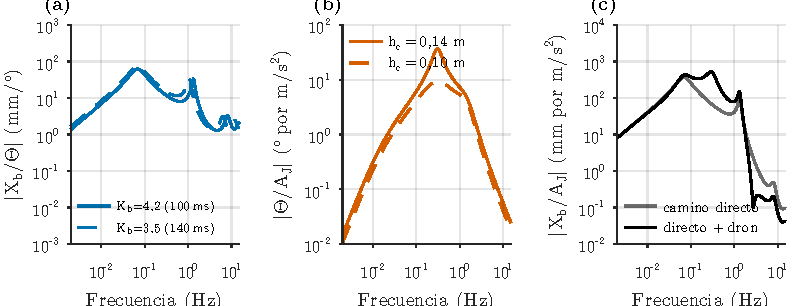
\includegraphics{figures/fig_transmissibility.pdf}
  \caption{Propagación de perturbaciones predicha por \eqref{eq:propag} (ganancias de vuelo estacionario, $k_T=1.42$). (a) Desplazamiento de la bola por grado de inclinación del octocóptero con el lazo de la bola cerrado. (b) Inclinación del octocóptero por unidad de aceleración de la base. (c) Desplazamiento de la bola por unidad de aceleración de la base, por el camino directo y a través del octocóptero.}
  \label{fig:transm}
\end{figure}

\subsection{Limitaciones fundamentales e implicaciones de diseño}
\label{sec:limits_fund}
El modelo también acota lo que cualquier controlador puede lograr con el hardware actual \cite{skogestad2005}.
\begin{itemize}
  \item \textbf{Octocóptero.} Un polo inestable $p$ exige un cruce por encima de $\approx2p$, y un retardo efectivo $\theta_e$ lo limita a $\approx1/\theta_e$; la estabilización robusta requiere aproximadamente $p\,\theta_e<0.5$. Con $p=\SI{6.1}{\radian\per\second}$ y $\theta_e\approx\tau_m+T_a=\SI{0.09}{\second}$, $p\theta_e=0.55$: el control de actitud del módulo en la rótula opera en el borde de este límite. El remedio estructural es bajar el centro de masa: con las baterías bajo la rótula ($h_c<0$) el módulo se vuelve un péndulo estable y la autoridad que exige \eqref{eq:thetastar} disminuye; además, las baterías bajas mejorarían el vuelco en la rampa.
  \item \textbf{\textit{Ball and plate}.} El cero en el semiplano derecho $z_1=\SI{15.2}{\radian\per\second}$ limita el cruce a $\approx z_1/2=\SI{7.6}{\radian\per\second}$, y el retardo de $\approx$\SI{0.1}{\second}, a $\approx\SI{10}{\radian\per\second}$; el PID opera en $K_{b,\mathrm{eff}}k_d\approx\SI{6}{\radian\per\second}$, cerca de ambas cotas, lo que explica el techo de $k_d$. Un control más rápido de la bola exige un retardo menor (servos digitales a \SI{333}{\hertz}, actualización de los servos sincronizada con los cuadros) y un $\kappa$ menor (la superficie del plato más cerca del centro de la junta universal).
  \item \textbf{Base.} El margen de aceleración \eqref{eq:tip} y el modo lento del octocóptero piden referencias suaves (con jerk limitado) para la base; en una pendiente de \SI{20}{\degree} el margen de aceleración sin empuje es de solo \SI{0.26}{\metre\per\second\squared}; con los rotores sosteniendo el 35--55\% del peso del módulo sube a 0,7--\SI{1.0}{\metre\per\second\squared} (Sección~\ref{sec:porquedron}). Las alternativas son un lastre bajo o un módulo aéreo más bajo.
  \item \textbf{Energía.} El margen de empuje cae con el cuadrado de la tensión de la batería (Sección~\ref{sec:bateria}); sin medición de tensión y compensación del colectivo, el tiempo útil de vuelo es de 3--\SI{7}{\minute} por par de LiPo.
\end{itemize}
   % 3. Modelo: acoplamiento, control y limites
%% ======================================================================
%% 05_design_files.tex -- 4. Resumen de archivos de diseno
%% ======================================================================
\section{Resumen de archivos de diseño}
\label{sec:designfiles}
Todos los archivos están en el repositorio \repourl. La Tabla~\ref{tab:designfiles} reúne los principales.

\begin{small}
\begin{longtable}{@{}>{\raggedright\arraybackslash}p{0.36\textwidth}>{\raggedright\arraybackslash}p{0.13\textwidth}>{\raggedright\arraybackslash}p{0.12\textwidth}>{\raggedright\arraybackslash}p{0.31\textwidth}@{}}
\caption{Resumen de archivos de diseño.}\label{tab:designfiles}\\
\toprule
Archivo & Tipo & Licencia & Ubicación / función \\
\midrule\endfirsthead
\toprule Archivo & Tipo & Licencia & Ubicación / función \\ \midrule\endhead
\texttt{junta nuevo de 8 motores con camara.step} & STEP (383 piezas) & CERN-OHL-S & \fn{02_cad/} (archivo externo, $>95$\,MB; \fn{.glb} en el repo) -- ensamble completo \\
\fn{x8_UAV_R350_imprimible_bandeja_v5.stp} & STEP & CERN-OHL-S & \fn{02_cad/} (archivo externo, $>95$\,MB) -- marco del octocóptero, torres y bandeja (impresión 3D) \\
\fn{ball_and_plate_camara.stp} & STEP & CERN-OHL-S & \fn{02_cad/recibidos/} -- plato, mecanismos de los servos, soporte de cámara \\
\fn{aerotray_conjunto_cad.xml} & MuJoCo XML & MIT & \fn{06_simulacion/simulacion/} -- modelo de rótula y guía (Isaac Lab, Sección~\ref{sec:flights}) \\
\fn{derive_ball.py}, \fn{derive_drone.py} & Python 3 (SymPy) & MIT & \fn{00_paper_HardwareX/.../scripts_modelo/} -- verificación simbólica de las ecuaciones de la Sección~\ref{sec:model} \\
\fn{analysis.py}, \fn{ball_dt.py}, \fn{chain.py}, \fn{params.py}, \fn{rampa.py}, \fn{bateria.py}, \fn{exportar_datos_matlab.py} & Python 3 & MIT & \fn{00_paper_HardwareX/.../scripts_modelo/} -- todas las cifras del modelo de las Secciones~\ref{sec:model} y \ref{sec:modelval} \\
\fn{generar_todas.m}, \fn{estilo_paper.m}, \fn{fig_*.m} & MATLAB & MIT & \fn{00_paper_HardwareX/.../figuras_matlab/} -- todas las figuras de datos y del modelo \\
\fn{Marcadores_ArUco_y_Calibracion_Bandeja_A4.pdf} & PDF & CC BY 4.0 & \fn{01_guias_y_documentacion/imprimibles/} -- hoja de calibración del plato \\
\fn{captura_octo_m8_vuelo_guia.ino} (v11) & Arduino C++ & MIT & \fn{03_firmware/firmware/} -- firmware de actitud, rumbo en base y vuelo en guía del octocóptero \\
\fn{captura_octo_m8_banco_angulo_laser.ino} & Arduino C++ & MIT & \fn{03_firmware/firmware/} -- firmware de banco (colectivo fijo) \\
\fn{ball_plate_esp32s3_platformio/src/main.cpp} & PlatformIO C++ & MIT & \fn{03_firmware/} -- PID de la bola y servos en la ESP32-S3 \\
\fn{seguidor.py}, \fn{comunicacion.py}, \fn{myrio_uart.py}, \fn{pagina_dron.py}, \fn{pagina_robot.py} & Python 3 & MIT & \fn{04_raspberry_pi/pi_control/} -- supervisor en la Raspberry Pi, visión, enlaces e interfaz web \\
\fn{config_pi.json}, \fn{ajustes.json}, \fn{arrancar.sh} & JSON, shell & MIT & \fn{04_raspberry_pi/pi_control/} -- configuración, ganancias y lazo de arranque \\
\fn{prueba_prueba.vi} (principal), \fn{AeroTray_Control_Formula.vi}, \fn{CONTROL_TRAYECTORIA.vi}, \fn{Laboratorio2_Ejercicio1_Motores.lvproj} & LabVIEW 2019 & MIT & \fn{05_labview_myrio/Control_Robot_Movil/} -- control de la base en la myRIO, odometría, secuencias, UART \\
\fn{cargar_vuelo_guia_desde_pi.sh}, \fn{subir_uart_a_pi.sh} & shell & MIT & \fn{03_firmware/firmware/}, \fn{04_raspberry_pi/pi_control/} -- grabar el dron y desplegar el código de la Pi \\
\fn{comparar_vuelo_isaac.py}, \fn{make_figures.py}, \fn{bp_metrics.py} & Python 3 & MIT & \fn{07_herramientas/}, \fn{00_paper_HardwareX/scripts_repositorio/} -- métricas y figuras de la Sección~\ref{sec:validation} \\
\fn{isaaclab_aerotray/} (\fn{env.py}, \fn{agent.py}) & Python & MIT & \fn{06_simulacion/simulacion/} -- tarea de Isaac Lab y agente PPO \\
\fn{vuelo_*.csv}, \fn{dron_log_*.csv}, \fn{registro_*.csv}, \fn{salida.log} & CSV, texto & CC BY 4.0 & \fn{08_datos_y_registros/} -- registros crudos usados en este artículo \\
\fn{GUIA_EQUIPO.md}, \fn{VUELO_GUIA.md}, \fn{UART_MYRIO.md} & Markdown & CC BY 4.0 & \fn{01_guias_y_documentacion/} -- procedimientos de operación y vuelo \\
Esquemáticos Proteus (\fn{AeroTray_Esquematicos.pdsprj}, \fn{AeroTray_Esquematicos_vista_v2.pdf}, \fn{AeroTray_Fig_Comunicaciones.pdf}) & Proteus, PDF & CERN-OHL-S & \fn{02_cad/esquematicos_proteus/} -- esquemático jerárquico de 6 hojas y comunicaciones (Sección~\ref{sec:power}) \\
\fn{IMG_1867.mov}, \fn{IMG_1868.mov}, \fn{IMG_1869.mov} & video HEVC 4K & CC BY 4.0 & Archivo externo (ver README) -- vuelos 6 y 7 del 20/11 (Sección~\ref{sec:flights}) \\
\bottomrule
\end{longtable}
\end{small}

        % 4. Archivos de diseno
%% ======================================================================
%% 06_bom.tex -- 5. Lista de materiales
%% ======================================================================
\section{Resumen de la lista de materiales}
\label{sec:bom}
La Tabla~\ref{tab:bom} reúne los componentes del prototipo final. Los costos son precios unitarios aproximados en USD a noviembre de 2026, de proveedores locales y en línea. Los elementos marcados como ``lab'' los proporcionó el laboratorio de la universidad; su precio de lista se da como referencia.

\begin{small}
\setlength{\tabcolsep}{4pt}
\begin{longtable}{@{}>{\raggedright\arraybackslash}p{0.27\textwidth}r>{\raggedleft\arraybackslash}p{0.08\textwidth}>{\raggedleft\arraybackslash}p{0.08\textwidth}>{\raggedright\arraybackslash}p{0.15\textwidth}>{\raggedright\arraybackslash}p{0.14\textwidth}@{}}
\caption{Lista de materiales (costos aproximados).}\label{tab:bom}\\
\toprule
Componente & Cant. & Unit. (USD) & Total (USD) & Fuente & Tipo de material \\
\midrule\endfirsthead
\toprule Componente & Cant. & Unit. (USD) & Total (USD) & Fuente & Tipo de material \\ \midrule\endhead
\multicolumn{6}{@{}l}{\emph{N1 -- Base móvil}}\\
NI myRIO-1900 & 1 & 500 & 500 & lab & Electrónica \\
Piezas del chasis TETRIX MAX, 2 motores TorqueNADO con encoder, ruedas y ruedas omnidireccionales & 1 juego & 230 & 230 & lab & Metal / electromec. \\
Puente H MDD10A ($\geq$\SI{10}{\ampere}/canal) & 1 & 15 & 15 & proveedor local & Electrónica \\
Batería NiMH TETRIX \SI{12}{\volt} \SI{3000}{\milli\ampere\hour} + fusible de \SI{20}{\ampere} & 1 & 45 & 45 & lab & Energía \\
Power bank \SI{5}{\volt}/\SI{3}{\ampere} + elevador de 5 a \SI{12}{\volt} & 1 & 25 & 25 & proveedor local & Energía \\
Mástil, guía vertical y carro (perfil de aluminio, piezas impresas) & 1 & 30 & 30 & local / impreso & Metal, PLA \\
\multicolumn{6}{@{}l}{\emph{N2 -- Módulo aéreo (octocóptero)}}\\
Marco (placa central y torres impresas, 8 brazos R350) & 1 & 60 & 60 & impreso / en línea & PLA, compuesto \\
Rótula esférica & 1 & 10 & 10 & proveedor local & Metal \\
Motor sin escobillas A2212 920\,KV & 8 & 18 & 144 & en línea & Electromec. \\
Hélice 9450 (par horaria/antihoraria) & 4 & 3 & 12 & en línea & Polímero \\
ESC 30\,A sin BEC & 8 & 10 & 80 & en línea & Electrónica \\
LiPo 3S \SI{3300}{\milli\ampere\hour} 25C & 2 & 35 & 70 & en línea & Energía \\
Portafusible ATO + fusible de \SI{30}{\ampere}, relé, condensador de \SI{1000}{\micro\farad}/\SI{25}{\volt}, cable 14 AWG, XT60 & 2 & 12 & 24 & proveedor local & Eléctrico \\
NodeMCU-32S (ESP32) & 1 & 8 & 8 & proveedor local & Electrónica \\
IMU MPU-6050 & 1 & 3 & 3 & proveedor local & Electrónica \\
Sensor de tiempo de vuelo VL53L0X & 1 & 5 & 5 & proveedor local & Electrónica \\
Reductor XL4015 & 2 & 4 & 8 & proveedor local & Electrónica \\
\multicolumn{6}{@{}l}{\emph{N3 -- Bandeja del \textit{ball and plate}}}\\
Cámara USB PS3 Eye & 1 & 10 & 10 & en línea & Electrónica \\
Placa de desarrollo ESP32-S3 & 1 & 12 & 12 & proveedor local & Electrónica \\
Servo Futaba S3003 & 2 & 10 & 20 & proveedor local & Electromec. \\
Plato ($250\times220$~mm), mecanismos, torres de cámara & 1 & 15 & 15 & impreso & PLA \\
Bola azul, \SI{27}{\milli\metre} & 1 & 1 & 1 & local & Polímero \\
\multicolumn{6}{@{}l}{\emph{N4 -- Supervisor, distribución electrónica y paro}}\\
Raspberry Pi 3B+ + \SI{32}{GB} microSD & 1 & 55 & 55 & en línea & Electrónica \\
Pack 3S 18650 con BMS (lógica BT5 y servos BT6) & 2 & 20 & 40 & proveedor local & Energía \\
Hongo de emergencia NC enclavable, cable mellizo \SI{4}{\metre}, relés K3--K4, diodos 1N4007, borneras Wago & 1 & 15 & 15 & proveedor local & Eléctrico \\
Cables USB, hub, conectores, tornillos, precintos & 1 & 20 & 20 & proveedor local & Varios \\
\midrule
\multicolumn{3}{@{}l}{\textbf{Total (todos los elementos)}} & \textbf{1457} & & \\
\multicolumn{3}{@{}l}{\textbf{Total sin los elementos del laboratorio}} & \textbf{682} & & \\
\bottomrule
\end{longtable}
\end{small}

\subsection{Viabilidad económica}
\label{sec:costos}
La Tabla~\ref{tab:costos} compara el módulo aéreo con alternativas que cumplen la misma función: nivelar el plato mientras la base sube una rampa. Los precios de las alternativas son referencias de mercado aproximadas.

\begin{table}[!htbp]
\centering
\small
\caption{Comparación de costo y funciones de las alternativas para la etapa de nivelación.}
\label{tab:costos}
\begin{tabularx}{\textwidth}{@{}>{\raggedright\arraybackslash}p{0.26\textwidth}c>{\raggedright\arraybackslash}X>{\raggedright\arraybackslash}p{0.13\textwidth}>{\raggedright\arraybackslash}p{0.12\textwidth}@{}}
\toprule
Alternativa & USD & Nivelación en 10° y 20° & Par contra la base & Lastre ajustable \\
\midrule
Solo servos en la base (2 S3003) & $\sim$20 & en 10° consume el \SI{93}{\percent} del recorrido; en 20° no es posible & sí & no \\
Cardán de servos + IMU (2 MG996R, MPU-6050) & $\sim$30--50 & sí & sí & no \\
Cardán \emph{brushless} (Storm32 + 2 motores) & $\sim$80--150 & sí, con carga útil limitada & sí & no \\
\textbf{Módulo octocóptero (Tabla~\ref{tab:bom})} & $\sim$\textbf{425} & sí, referida a la gravedad & \textbf{no} (rótula) & \textbf{sí} ($f=0$--1) \\
Equipos comerciales de laboratorio de un solo problema (\emph{ball balancer}, dron de 3 GDL) & miles & no son móviles & --- & --- \\
\bottomrule
\end{tabularx}
\end{table}

Solo para nivelar, un cardán de servos es entre 8 y 14 veces más barato. El octocóptero se justifica por tres funciones que el cardán no tiene:
\begin{itemize}
  \item no le transmite a la bola la reacción de la base;
  \item deja libre el recorrido de los servos para controlar la bola;
  \item su empuje es un lastre ajustable que baja el centro de masa y sube la pendiente de vuelco (Sección~\ref{sec:porquedron}).
\end{itemize}
Además, convierte el robot en una plataforma de investigación de equilibrios apilados. El costo total sigue siendo muy inferior al del equipo comercial de laboratorio, que resuelve un solo problema sobre una base fija.
                 % 5. Lista de materiales
%% ======================================================================
%% 07_build.tex -- 6. Instrucciones de construccion
%% ======================================================================
\section{Instrucciones de construcción}
\label{sec:build}

\paragraph{Herramientas}
\begin{itemize}
  \item llaves hexagonales y llaves TETRIX;
  \item cautín, crimpadora para conectores XT60 y Dupont, multímetro y pinza amperimétrica de DC;
  \item impresora 3D FDM (PLA, capa de 0,2\,mm, 30\% de relleno para las torres y los mecanismos);
  \item una laptop con Arduino CLI (núcleo ESP32), PlatformIO y LabVIEW 2019 con el toolkit de myRIO.
\end{itemize}

\paragraph{Seguridad}
Ensamblar y grabar con las LiPo desconectadas y sin hélices. Comprobar el sentido de giro de cada motor sin hélices antes del primer vuelo.

\begin{figure}[!htbp]
  \centering
  \begin{subfigure}[b]{0.24\textwidth}\centering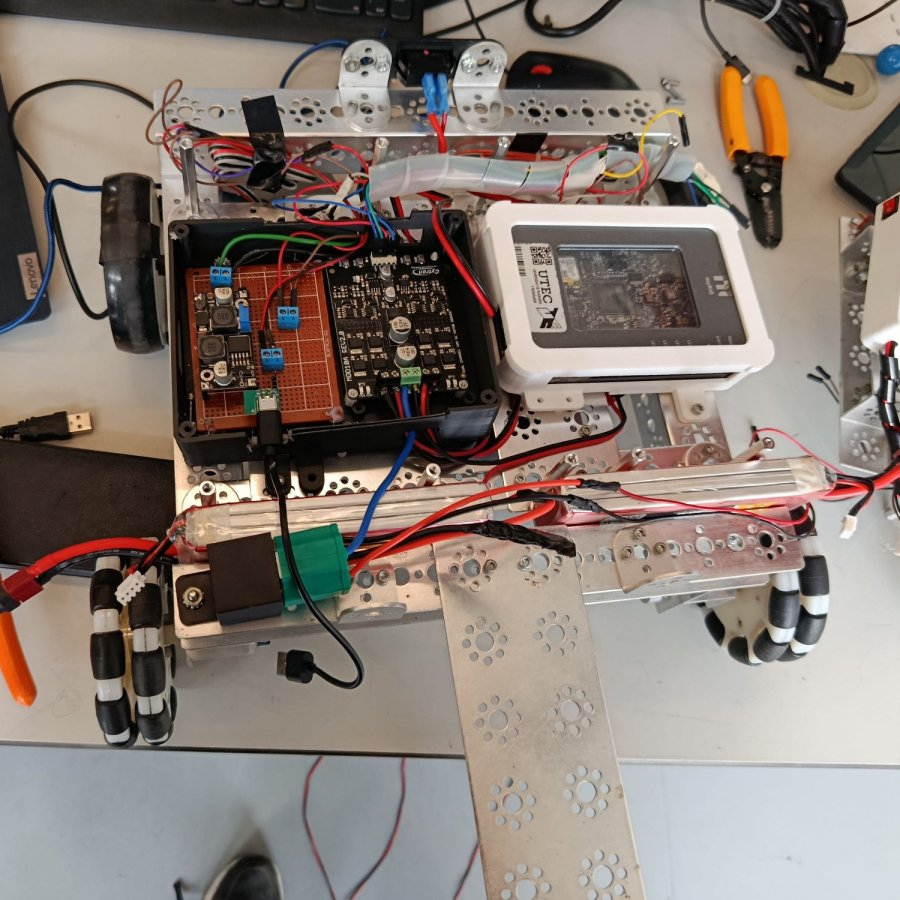
\includegraphics[width=\linewidth]{figures/paso1_base.jpg}\caption{Paso 1: base móvil (myRIO, MDD10A, LiPo).}\end{subfigure}\hfill
  \begin{subfigure}[b]{0.24\textwidth}\centering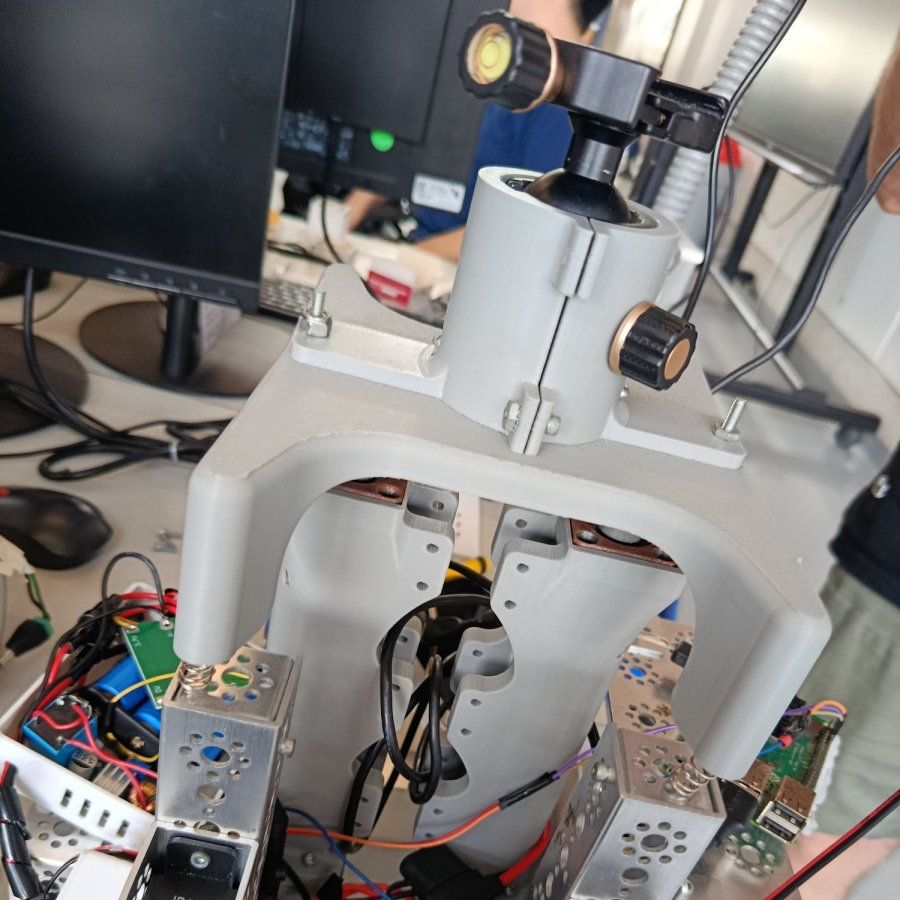
\includegraphics[width=\linewidth]{figures/paso2_mastil.jpg}\caption{Paso 2: mástil, guía y rótula.}\end{subfigure}\hfill
  \begin{subfigure}[b]{0.24\textwidth}\centering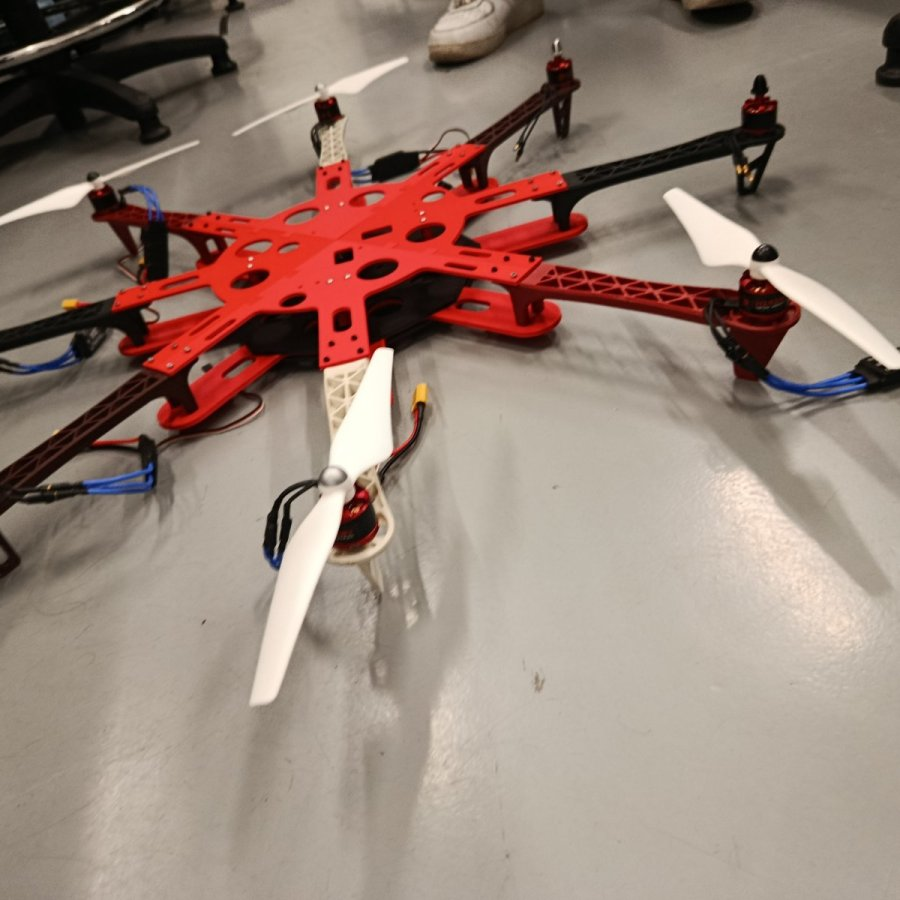
\includegraphics[width=\linewidth]{figures/paso3_marco.jpg}\caption{Paso 3: marco de ocho brazos.}\end{subfigure}\hfill
  \begin{subfigure}[b]{0.24\textwidth}\centering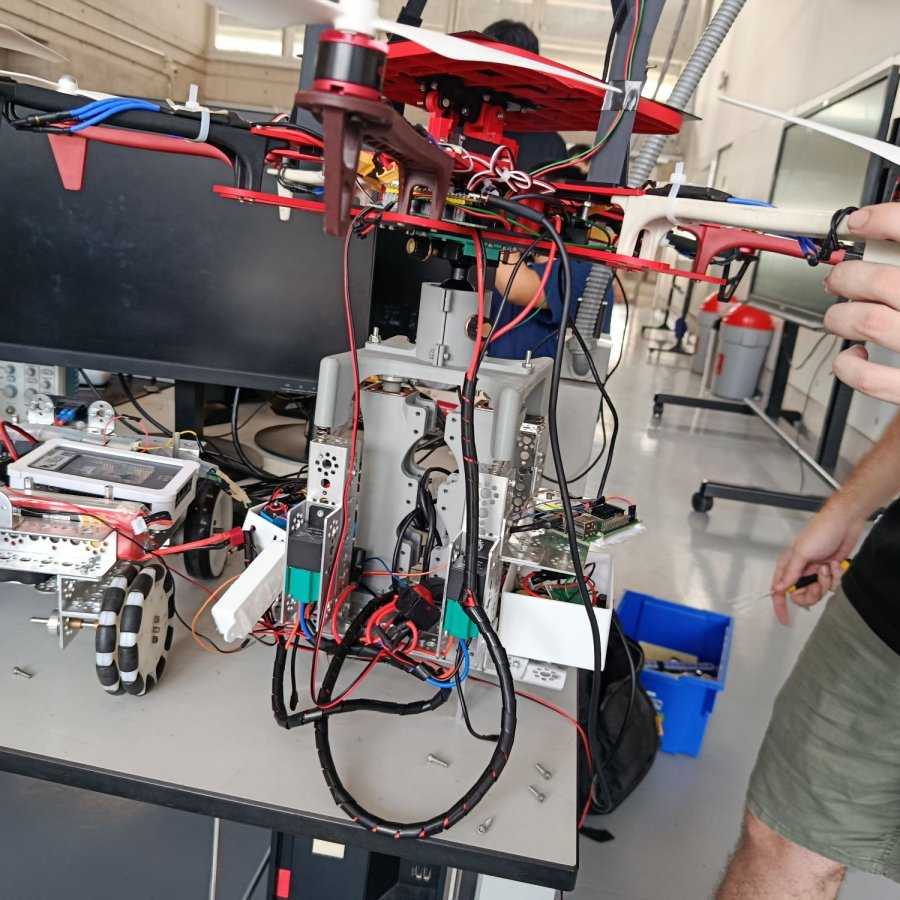
\includegraphics[width=\linewidth]{figures/paso4_dron_rotula.jpg}\caption{Paso 4: montaje del dron en la rótula.}\end{subfigure}\\[2mm]
  \begin{subfigure}[b]{0.24\textwidth}\centering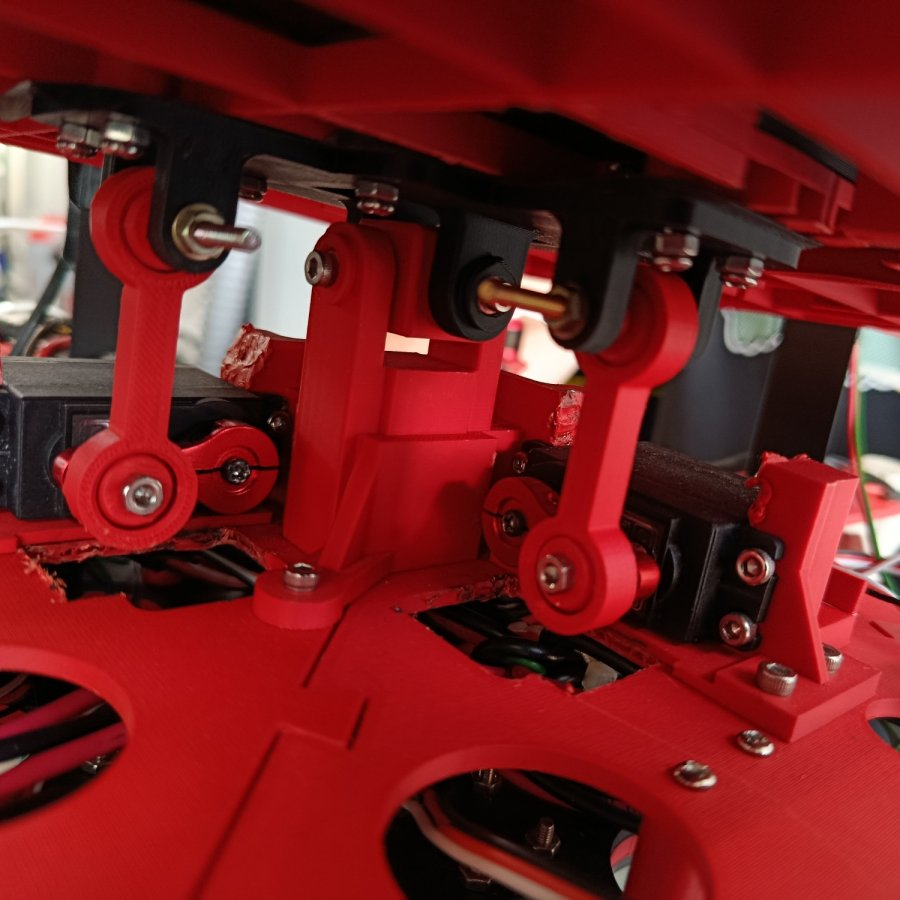
\includegraphics[width=\linewidth]{figures/paso5_mecanismo.jpg}\caption{Paso 5: servos y bielas de la bandeja.}\end{subfigure}\hfill
  \begin{subfigure}[b]{0.24\textwidth}\centering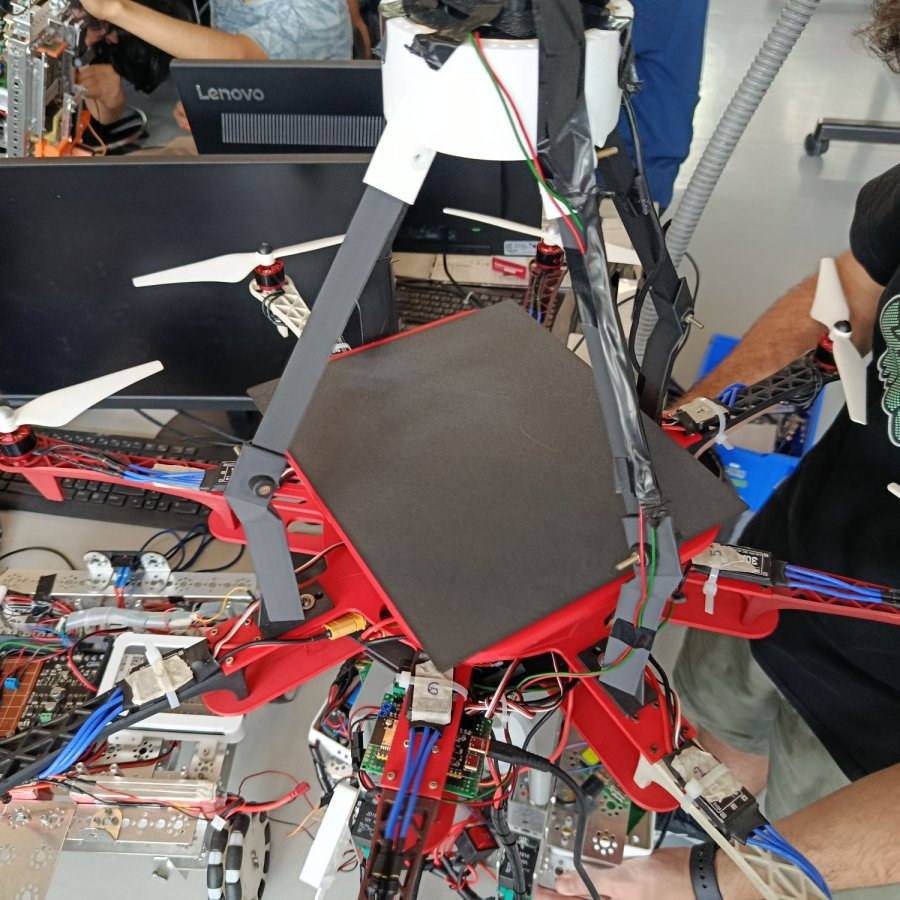
\includegraphics[width=\linewidth]{figures/paso5_bandeja_camara.jpg}\caption{Paso 5: plato y torres de la cámara.}\end{subfigure}\hfill
  \begin{subfigure}[b]{0.24\textwidth}\centering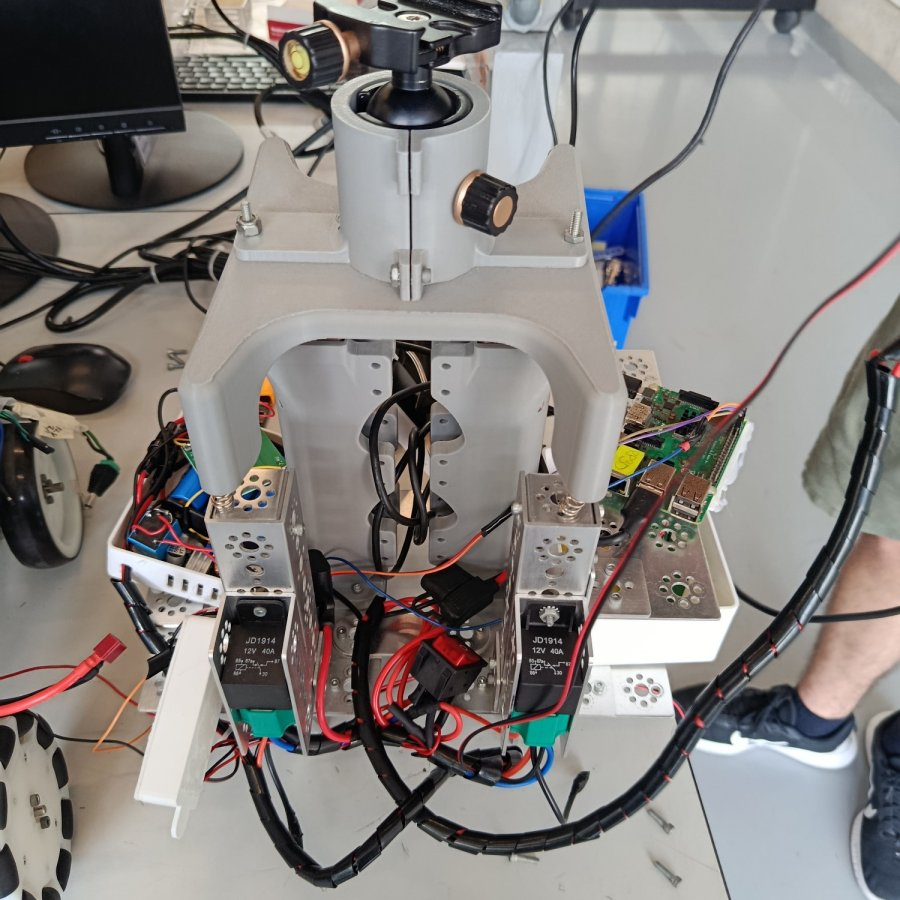
\includegraphics[width=\linewidth]{figures/paso6_supervisor.jpg}\caption{Paso 6: relés de paro y Raspberry Pi.}\end{subfigure}\hfill
  \begin{subfigure}[b]{0.24\textwidth}\centering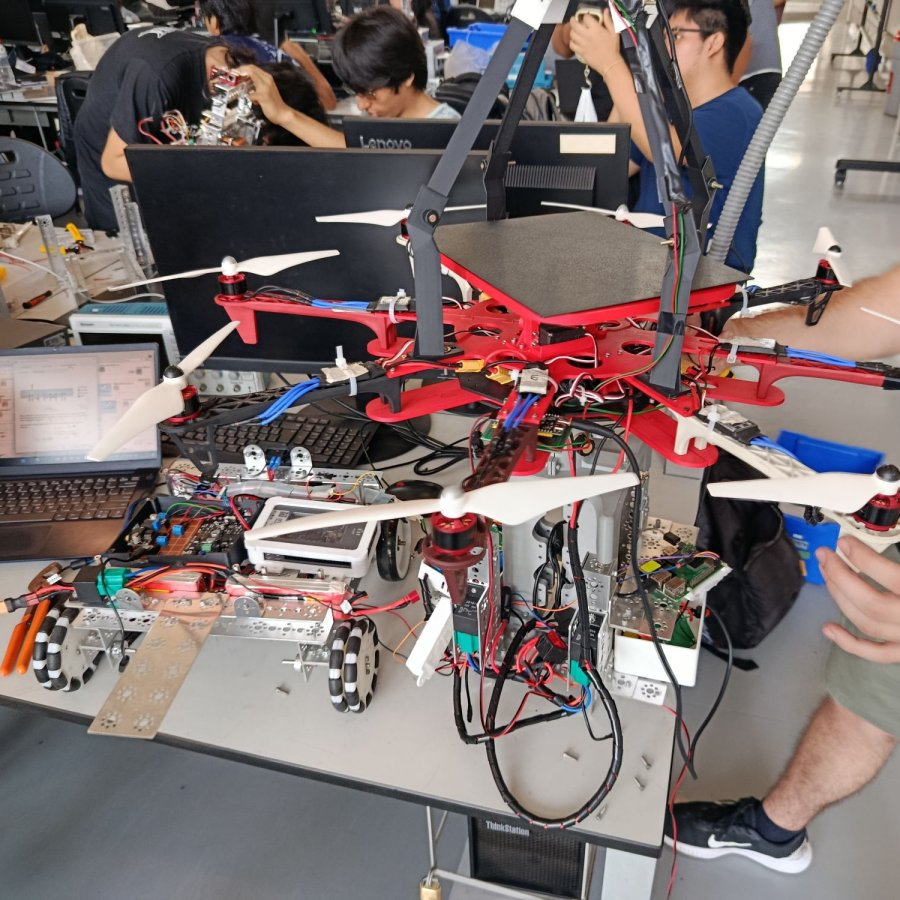
\includegraphics[width=\linewidth]{figures/paso7_integracion.jpg}\caption{Paso 8: integración.}\end{subfigure}
  \caption{Secuencia de construcción del prototipo final de AeroTray.}
  \label{fig:build}
\end{figure}

\begin{enumerate}[label=\textbf{Paso \arabic*.}, leftmargin=*, align=left]
  \item \textbf{Base móvil (Fig.~\ref{fig:build}a).}
  \begin{enumerate}[label=(\alph*)]
    \item Armar el chasis TETRIX con los dos motores TorqueNADO en el eje trasero y las ruedas omnidireccionales adelante.
    \item Medir la trocha (centro a centro de las ruedas motrices). Debe coincidir con el valor del nodo de fórmula de LabVIEW, \SI{0.3794}{\metre}.
    \item Cablear el motor izquierdo al MXP-A de la myRIO (PWM0 en el pin 27, dirección en DIO0, pin 11, encoder en ENC A/B) y el derecho al MXP-B con los mismos pines, a través del MDD10A.
    \item Proteger la NiMH con el fusible de \SI{20}{\ampere} y pasarla por el contacto del relé K3.
    \item \emph{Comprobación:} con las ruedas levantadas, ordenar avance y verificar que ambos contadores de encoder aumentan. El contador derecho se invierte por software.
  \end{enumerate}

  \item \textbf{Mástil, guía y rótula (Fig.~\ref{fig:build}b).}
  \begin{enumerate}[label=(\alph*)]
    \item Fijar el mástil vertical sobre el eje motriz y montar la guía vertical.
    \item Insertar el carro con la rótula esférica y verificar unos \SI{140}{\milli\metre} de recorrido libre.
    \item Poner topes blandos en ambos extremos de la guía.
    \item \emph{Comprobación:} el carro debe caer libremente por su propio peso; la fricción de la guía sesga la identificación por despegue de la Sección~\ref{sec:ident}.
  \end{enumerate}

  \item \textbf{Marco del octocóptero y alimentación (Fig.~\ref{fig:build}c).}
  \begin{enumerate}[label=(\alph*)]
    \item Imprimir la placa central y las torres (archivo\\ \fn{x8_UAV_R350_imprimible_bandeja_v5.stp}) y montar los ocho brazos cada \SI{45}{\degree}: M8 en $+x$, M7 en $+y$.
    \item Instalar M1--M4 con giro horario y M5--M8 con giro antihorario (Tabla~\ref{tab:params}).
    \item Armar las dos ramas de potencia independientes del esquema Rev.~I (Sección~\ref{sec:power}), cada una con LiPo, XT60, fusible ATO de \SI{30}{\ampere}, contacto 30--87 del relé (K1, K2), par trenzado 14\,AWG y condensador de \SI{1000}{\micro\farad} en el dron. La rama A alimenta los ESC 1, 3, 5 y 7, y la rama B los ESC 2, 4, 6 y 8; unir solo las tierras, y solo en el dron.
    \item Cortar el cable rojo (BEC) de los ESC.
    \item Conectar las señales de los ESC según la Tabla~\ref{tab:pins} (firmware v11): GPIO 25, 26, 27, 14, 21, 19, 5 y 17 para M1--M8 de la NodeMCU-32S; la MPU-6050 y el VL53L0X al I$^2$C (SDA 23, SCL 22).
    \item Alimentar la NodeMCU por el hub USB (dominio de lógica). No sumar un regulador desde la LiPo: serían dos fuentes de \SI{5}{\volt} en paralelo.
    \item Opcional, recomendado: soldar los divisores de VBAT hacia GPIO34/35 con R1 = R3 = \SI{10}{\kilo\ohm} y R2 = R4 = \SI{3.3}{\kilo\ohm} ($\div4{,}03$) y \SI{100}{\nano\farad} a GND, para que una versión futura del firmware mida la tensión (Sección~\ref{sec:bateria}).
  \end{enumerate}

  \item \textbf{Dron en la rótula (Fig.~\ref{fig:build}d).}
  \begin{enumerate}[label=(\alph*)]
    \item Atornillar el marco a la rótula de modo que el centro de la rótula coincida con el centro del marco.
    \item Equilibrar el conjunto: con los motores apagados debe quedar nivelado. Mover las baterías hasta lograrlo, y mantenerlas lo más bajas posible, porque la altura del centro de masa sobre la rótula fija la inestabilidad del módulo (Sección~\ref{sec:limits_fund}). El prototipo aún tiene una excentricidad residual de \SI{9.5}{\milli\metre} hacia M8, identificada en la Sección~\ref{sec:ident}.
  \end{enumerate}

  \item \textbf{Bandeja (Fig.~\ref{fig:build}e,f).}
  \begin{enumerate}[label=(\alph*)]
    \item Imprimir el plato, los mecanismos y las cuatro torres de la cámara.
    \item Montar los dos servos S3003 y conectar las señales a GPIO47 ($x$) y GPIO21 ($y$) de la ESP32-S3.
    \item Alimentar los servos desde el dominio S5 (BT6, XL4015, contacto de K4) con \SI{1000}{\micro\farad} en la entrada y tierra común con la ESP32-S3; no unir el pin de \SI{5}{\volt} de la ESP32-S3 a ese riel.
    \item Fijar la PS3 Eye en las torres, centrada sobre el plato, y ajustar el neutro del plato con los mecanismos hasta que quede nivelado en unos \SI{1390}{\micro\second}.
  \end{enumerate}

  \item \textbf{Supervisor y paro (Fig.~\ref{fig:build}g).}
  \begin{enumerate}[label=(\alph*)]
    \item Instalar Raspberry Pi OS (Debian 13) y crear un entorno virtual \texttt{\textasciitilde/venv} con \texttt{opencv-python}, \texttt{numpy}, \texttt{pyserial} y \texttt{esptool}.
    \item Copiar \texttt{pi\_control/} a la carpeta personal.
    \item Habilitar la UART física: en \texttt{raspi-config}, poner el \emph{login shell} serie en \emph{No} y el hardware serie en \emph{Sí}, y reiniciar.
    \item Cablear GPIO14 (TX, pin 8) al pin 10 (RX) del MXP-A, GPIO15 (RX, pin 10) al pin 14 (TX) del MXP-A, y tierra (pin 6) al pin 12 del MXP-A.
    \item Alimentar la Pi desde su propio pack 3S 18650 (BT5) y un XL4015 ajustado a \SI{5.2}{\volt}.
    \item Cablear la caja de mando: hongo SB1 (NC, enclavable) en serie con las bobinas de K1--K4 desde BT6 por un fusible de \SI{1}{\ampere}, con un diodo 1N4007 en antiparalelo con cada bobina. \emph{Comprobación:} con SB1 pulsado, ninguna rama debe tener tensión aguas abajo de su relé.
  \end{enumerate}

  \item \textbf{Firmware.}
  \begin{enumerate}[label=(\alph*)]
    \item Compilar el firmware del dron:\\ \texttt{arduino-cli compile --fqbn esp32:esp32:nodemcu-32s}.
    \item Grabarlo desde la Pi (\fn{cargar_vuelo_guia_desde_pi.sh}), que usa \texttt{esptool write-flash 0x0}.
    \item Grabar la ESP32-S3 con PlatformIO.
    \item Desplegar el proyecto de LabVIEW en la myRIO (\fn{prueba_prueba.vi} como VI principal).
  \end{enumerate}

  \item \textbf{Comprobaciones de integración (Fig.~\ref{fig:build}h).}
  \begin{enumerate}[label=(\alph*)]
    \item Lanzar \texttt{arrancar.sh} y abrir \url{http://<ip-de-la-pi>:8080/robot}. El registro debe mostrar el encabezado del firmware del dron, ``UART conectada en /dev/serial0'' y la tasa de la cámara.
    \item Con la batería desconectada, enviar \emph{cal} y verificar ``CAL OK''.
    \item Colocar la bola y verificar que se detecta en las cuatro esquinas del plato.
  \end{enumerate}
\end{enumerate}
               % 6. Instrucciones de construccion
%% ======================================================================
%% 08_operation.tex -- 7. Instrucciones de operacion
%% ======================================================================
\section{Instrucciones de operación}
\label{sec:operation}

\begin{figure}[!htbp]
  \centering
  \begin{subfigure}[b]{0.52\textwidth}\centering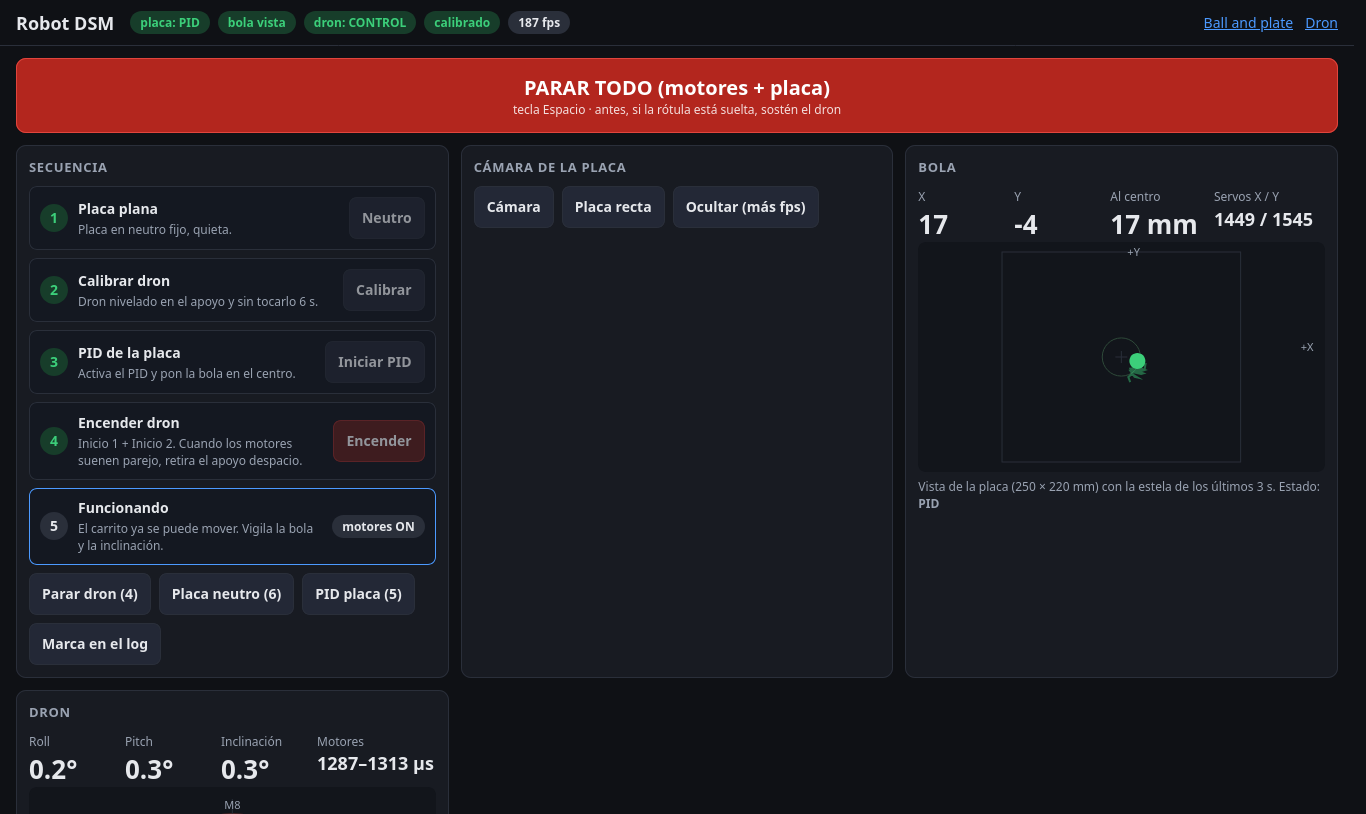
\includegraphics[width=\linewidth]{figures/ui_robot_page.png}\caption{Página web \texttt{/robot} servida por la Pi.}\end{subfigure}\hfill
  \begin{subfigure}[b]{0.45\textwidth}\centering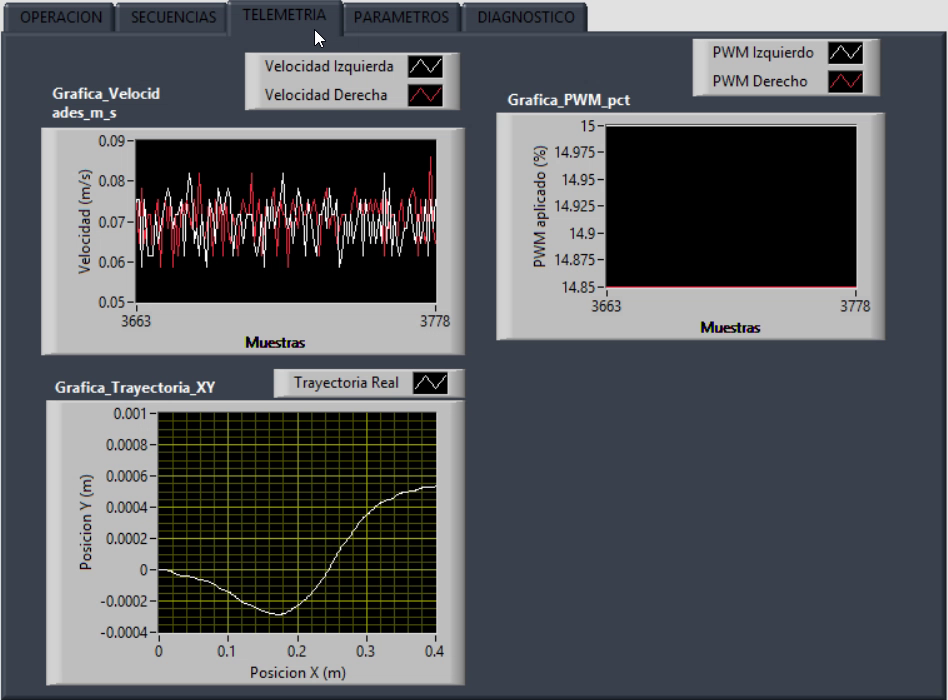
\includegraphics[width=\linewidth]{figures/ui_labview_telemetry.png}\caption{Pestaña de telemetría de LabVIEW (myRIO).}\end{subfigure}
  \caption{Interfaces del operador. La página web muestra el estado del plato, de la bola y del dron, una secuencia guiada de arranque y un botón de PARAR TODO (también la barra espaciadora); el panel de LabVIEW muestra las velocidades de las ruedas, el PWM y la trayectoria $x$--$y$.}
  \label{fig:ui}
\end{figure}

\paragraph{Requisitos previos}
\begin{itemize}
  \item baterías cargadas: las dos LiPo a \SI{12.6}{\volt} en reposo y con menos de \SI{0.05}{\volt} de diferencia entre sí, la NiMH, los dos packs 18650 y el power bank;
  \item hélices revisadas y ajustadas;
  \item guía libre, con ambos topes en su lugar;
  \item una laptop o un celular en la misma red Wi-Fi que la Pi;
  \item dos operadores: uno en la página web, con la barra espaciadora como parada inmediata, y otro mirando el robot con el hongo de emergencia SB1 a mano;
  \item lentes de seguridad para todas las personas a menos de \SI{2}{\metre}.
\end{itemize}

\paragraph{Secuencia de arranque}
La Fig.~\ref{fig:fsm_dron} resume la máquina de estados del firmware v11 del octocóptero que gobierna el arranque, el vuelo en guía y los cortes de seguridad.
\begin{enumerate}
  \item Con SB1 pulsado, encender la lógica (SW1). \texttt{arrancar.sh} lanza \texttt{seguidor.py} y lo reinicia si se detiene. Esperar a que la NodeMCU arranque: así los pulsos que emiten GPIO5 y GPIO14 durante el arranque no llegan a ESC energizados.
  \item Encender la myRIO y lanzar el VI de LabVIEW. El módulo UART debe mostrar la posición recibida de la bola y los ángulos del dron (Fig.~\ref{fig:ui}b).
  \item En \texttt{/robot}:
  \begin{enumerate}[label=\alph*.]
    \item poner el plato en \emph{Neutro};
    \item con el dron nivelado y quieto, pulsar \emph{Calibrar} y esperar 5\,s hasta ``CAL OK'';
    \item pulsar \emph{Iniciar PID} con la bola cerca del centro.
  \end{enumerate}
  \item Medir la tensión en reposo de las dos LiPo, anotarla y conectarlas. Soltar SB1 (cierran K1--K4). Pulsar \emph{Armar e iniciar motores}: el colectivo sube en rampa a \SI{1300}{\micro\second} (ralentí) y el lazo de actitud queda activo.
  \item \textbf{Modo banco} (base en movimiento, dron en ralentí). Mover la base desde LabVIEW con una orden manual, un objetivo de distancia, el giro de \SI{360}{\degree}, ir a un punto o una secuencia cargada.
  \item \textbf{Modo rampa} (propuesto, Sección~\ref{sec:porquedron}). Antes de la rampa, subir el colectivo con \emph{Subir} hasta 1450--\SI{1550}{\micro\second} ($f\approx0.35$--0,55): el módulo sigue apoyado, pero los rotores sostienen parte de su peso. Bajar a \SI{1300}{\micro\second} al terminar la subida. Por encima de \SI{1500}{\micro\second} el firmware limita el tramo a \SI{90}{\second}.
  \item \textbf{Vuelo en guía.} Pulsar \emph{Flotar}: el colectivo sube a \SI{25}{\micro\second\per\second}, a \SI{8}{\micro\second\per\second} por encima de \SI{1650}{\micro\second}, hasta \SI{1750}{\micro\second}. Si el módulo no despega, usar \emph{Subir} ($+$\SI{25}{\micro\second}) y anotar el colectivo de despegue; si pasa de \SI{1825}{\micro\second}, aterrizar y cambiar las baterías (Sección~\ref{sec:bateria}). Usar \emph{Subir/Bajar} ($\pm$\SI{25}{\micro\second}) y \emph{Mantener}; terminar con \emph{Aterrizar}, que baja a \SI{60}{\micro\second\per\second}.
\end{enumerate}

\begin{figure}[!htbp]
\centering
\begin{tikzpicture}[font=\footnotesize, >=Latex,
  st/.style={draw, rounded corners=3pt, align=center, minimum height=11.5mm, inner xsep=3.5pt, inner ysep=3pt, line width=0.7pt},
  stOff/.style={st, draw=pGris!90!black, fill=pGris!12, line width=1.1pt, text width=2.80cm},
  stPre/.style={st, draw=pOcre, fill=pOcre!10, text width=2.55cm},
  stVis/.style={st, draw=pAzul, fill=pAzul!8, text width=2.65cm},
  stArm/.style={st, draw=pOcre, fill=pOcre!12, text width=2.45cm},
  stRmp/.style={st, draw=pAzul, fill=pAzul!10, text width=2.65cm},
  stSub/.style={st, draw=pVerde!90!black, fill=white, minimum height=15mm, text width=4.85cm},
  stCut/.style={st, draw=pRojo, fill=pRojo!8, align=left, text width=4.68cm, line width=0.85pt, inner xsep=3pt, inner ysep=2pt, font=\footnotesize\linespread{0.95}\selectfont},
  tr/.style={->, line width=0.8pt, pAzul!90!black, rounded corners=2.5pt},
  trG/.style={->, line width=0.8pt, pVerde!85!black, rounded corners=2.5pt},
  trR/.style={->, line width=0.95pt, pRojo, rounded corners=2.5pt},
  lbl/.style={font=\footnotesize, align=center, inner sep=1.5pt}]

  % ---- Nivel 1: Preparacion (y = 0.00, ancho total 0.00..13.50 cm <= 13.74 cm)
  \node[stPre] (cal) at (1.42, 0.00) {\textbf{CAL}\\ \SI{5}{\second} inmóvil\\ (1000 muestras)};
  \node[stOff] (off) at (6.75, 0.00) {\textbf{DESARMADO}\\ (\texttt{OFF}, \SI{1000}{\micro\second})};
  \node[stVis] (vis) at (12.02, 0.00) {\textbf{VISTA}\\ (\texttt{PREVIEW},\\ \SI{1000}{\micro\second})};

  % Flecha de inicio hacia DESARMADO
  \fill[pGris!90!black] (6.75, 1.20) circle (0.08);
  \draw[->, thick, pGris!90!black] (6.75, 1.13) -- node[right=2pt]{\texttt{setup()}} (off.north);

  % Transiciones Nivel 1 (huecos 2.85..5.20 = 2.35 cm y 8.30..10.55 = 2.25 cm)
  \draw[tr]  ([yshift=2.4mm]off.west) -- node[lbl, above=1.5pt]{\texttt{cal} ($\ge\SI{4}{\second}$)} ([yshift=2.4mm]cal.east);
  \draw[tr]  ([yshift=-2.4mm]cal.east) -- node[lbl, below=1.5pt]{CAL OK\\ o rechazada} ([yshift=-2.4mm]off.west);
  \draw[tr]  ([yshift=2.4mm]off.east) -- node[lbl, above=1.5pt]{\texttt{vista} (cal.)} ([yshift=2.4mm]vis.west);
  \draw[trR] ([yshift=-2.4mm]vis.west) -- node[lbl, below=1.5pt, pRojo]{\texttt{parar} / \texttt{!}} ([yshift=-2.4mm]off.east);

  % ---- Nivel 2: Seguridad (izq), ARMADO (centro), RAMPA (der) (y = -3.65)
  \node[stCut] (cut) at (2.48, -3.72) {%
    \textbf{\textcolor{pRojo}{Cortes de seguridad}}\\
    $\bullet$ \texttt{parar}, \texttt{!} u orden inválida\\
    $\bullet$ inclinación $\ge\SI{12}{\degree}$\\
    $\bullet$ guiñada $\ge20^\circ$$^\ast$\\
    $\bullet$ giro $\ge35^\circ$/s$^\ast$\\
    $\bullet$ error I$^2$C o PWM\\
    $\bullet$ IMU lenta; ciclo $>\SI{30}{\milli\second}$\\
    {\scriptsize $^\ast$en ralentí: ventana $\pm20^\circ$, $120^\circ$/s}};
  \node[stArm] (arm) at (7.45, -3.65) {\textbf{ARMADO}\\ espera \texttt{iniciar}\\ (límite \SI{10}{\second})};
  \node[stRmp] (rmp) at (12.02, -3.65) {\textbf{RAMPA}\\ $1000\to\SI{1300}{\micro\second}$\\ ($+5\us/\SI{20}{\milli\second}$)};

  % Transiciones Nivel 1 <-> Nivel 2 (espacio vertical -0.65..-2.55)
  % DESARMADO y VISTA comparten la transicion arm BANCO_FIJO hacia ARMADO
  \draw[tr]  ([xshift=7mm]off.south) -- node[lbl, right=2pt, pos=0.62, align=left]{\texttt{arm BANCO\_FIJO}\\ (cal., $\le\SI{4}{\degree}$, $\le\SI{5}{\degree\per\second}$)} (arm.north);
  \draw[tr]  (vis.south) -- ++(0,-0.48) -| ([xshift=7mm]off.south |- 0,-1.35);
  % Timeout 10 s de ARMADO a DESARMADO (izquierda de arm.north)
  \draw[trR] ([xshift=-8mm]arm.north) -- node[lbl, left=2pt, pos=0.52, pRojo]{\SI{10}{\second}} ([xshift=-1mm]off.south);
  % Salida de Cortes hacia DESARMADO (etiqueta limpia sobre el codo, bien arriba de cut.north)
  \draw[trR] ([xshift=19mm]cut.north) -- (4.38,-1.52) -| ([xshift=-10mm]off.south);
  \node[lbl, pRojo, left=3pt, align=right] at (4.34, -1.68) {\texttt{stop()} $\to\SI{1000}{\micro\second}$};
  % Parada desde ARMADO hacia Cortes
  \draw[trR] (arm.west) -- node[lbl, above=1.5pt, pRojo]{\texttt{parar}} (cut.east |- arm.west);
  % ARMADO -> RAMPA (hueco 8.80..10.55 = 1.75 cm)
  \draw[tr]  (arm.east) -- node[lbl, above=1.5pt]{\texttt{iniciar}} node[lbl, below=1.5pt, align=center]{$<\SI{10}{\second}$\\ $\le\SI{4}{\degree}$} (rmp.west);

  % ---- Nivel 3: Contenedor CONTROL (y = -6.30..-13.25, ancho 0.00..13.50 cm)
  \node[stSub] (flt) at (2.82, -7.85) {\textbf{Flotar / colectivo manual}\\ \texttt{flotar} (\SI{1750}{\micro\second}), \texttt{maximo} (\SI{1950}{\micro\second})\\ \texttt{subir}/\texttt{bajar} ($\pm\SI{25}{\micro\second}$); exige \texttt{hb}};
  \node[stSub] (ral) at (10.68, -7.85) {\textbf{Ralentí / base}\\ \SI{1300}{\micro\second}; ventana $\pm\SI{20}{\degree}$\\ (corte guiñada \SI{120}{\degree\per\second})};
  \node[stSub] (alt) at (2.82, -11.20) {\textbf{Mantener altura}\\ \texttt{mantener} ($\sigma<\SI{30}{\milli\metre}$)\\ Kalman + cascada $\pm\SI{60}{\micro\second}$\\ \texttt{subir}/\texttt{bajar} $\pm\SI{20}{\milli\metre}$};
  \node[stSub] (atr) at (10.68, -11.20) {\textbf{Aterrizar}\\ \texttt{aterrizar} $\to$ rampa $-\SI{60}{\micro\second\per\second}$\\ hacia \SI{1300}{\micro\second}};

  % Nota de vigilancias dentro de CONTROL (centrada sin justificacion forzada)
  \node[font=\footnotesize, text=pVerde!75!black, align=center] (vig) at (6.75, -12.82)
    {Vigilancias automáticas: sin \texttt{hb} \SI{1.5}{\second} o $>\SI{1500}{\micro\second}$ por \SI{90}{\second} $\to$ \SI{1300}{\micro\second};\\
     $>\SI{1850}{\micro\second}$ por \SI{20}{\second} $\to$ \SI{1750}{\micro\second}.};

  % Marco contenedor de CONTROL en capa de fondo
  \begin{scope}[on background layer]
    \node[draw=pVerde, fill=pVerde!6, rounded corners=4pt, line width=1pt,
          fit=(flt)(ral)(alt)(atr)(vig), inner xsep=6pt, inner ysep=8pt,
          yshift=3.8mm] (ctrl) {};
  \end{scope}
  \node[font=\footnotesize\bfseries, text=pVerde!85!black, anchor=north west]
    at ([xshift=5pt, yshift=-2.5pt]ctrl.north west) {CONTROL (lazo de actitud a \SI{200}{\hertz}, colectivo 1300--\SI{1950}{\micro\second})};

  % Entrada RAMPA -> CONTROL (Ralenti) (etiqueta a la derecha de la flecha azul, lejos de la roja)
  \draw[tr] ([xshift=1mm]rmp.south) -- (ral.north -| 12.12,0);
  \node[lbl, right=2pt, align=left] at (12.15, -5.00) {\SI{1300}{\micro\second}\\ (\SI{1.2}{\second})};

  % Transiciones internas dentro de CONTROL (amplio espacio vertical -8.70..-10.35)
  \draw[trG] (ral.west) -- node[lbl, above=1.5pt]{\texttt{flotar}, \texttt{subir}} node[lbl, below=1.5pt]{(con \texttt{hb})} (flt.east);
  \draw[trG] ([xshift=-4mm]flt.south) -- node[lbl, left=2pt, align=right]{\texttt{mantener}\\ ($\sigma<\SI{30}{\milli\metre}$)} ([xshift=-4mm]alt.north);
  \draw[trG] ([xshift=6mm]alt.north) -- node[lbl, right=2pt, align=left]{otra orden o\\ láser $>\SI{2}{\second}$} ([xshift=6mm]flt.south);
  \draw[trG] ([yshift=-4mm]flt.east) -- (5.80,-8.25) |- ([yshift=2mm]atr.west);
  \node[lbl, text=pVerde!85!black, above=1.5pt, align=center] at (7.00,-11.00) {\texttt{aterrizar} /\\ vigilancia};
  \draw[trG] ([yshift=-2.5mm]alt.east) -- ([yshift=-2.5mm]atr.west);
  \draw[trG] (atr.north) -- node[lbl, right=2pt]{llega a \SI{1300}{\micro\second}} (ral.south);

  % Salidas de seguridad desde RAMPA y CONTROL hacia Cortes (en pasillo libre -5.65)
  \draw[trR] ([xshift=-10mm]rmp.south) -- (11.02,-5.68) -| ([xshift=14mm]cut.south);
  \draw[trR] (ctrl.north -| 2.15,0) -- node[lbl, left=2pt, pRojo]{corte / \texttt{parar}} (cut.south -| 2.15,0);
\end{tikzpicture}
\vspace{-4pt}
\caption{\raggedright Máquina de estados del firmware v11 del octocóptero (\texttt{captura\_octo\_m8\_vuelo\_guia.ino}). Funciones por transición: inicio en \texttt{DESARMADO} (\texttt{setup()}); órdenes serie \texttt{cal}, \texttt{vista}, \texttt{arm BANCO\_FIJO}, \texttt{iniciar}, \texttt{flotar}, \texttt{maximo}, \texttt{subir}, \texttt{bajar}, \texttt{mantener}, \texttt{aterrizar}, \texttt{parar} y orden rechazada (\texttt{command()}); parada \texttt{!} y línea inválida (\texttt{serialInput()}); fin de calibración (\texttt{collectCalibration()}); vencimiento de \SI{10}{\second} en \texttt{ARMADO}, paso de \texttt{RAMPA} a \texttt{CONTROL} (\SI{1300}{\micro\second}) y fallo MCPWM (\texttt{loop()}); colectivo y latido \texttt{hb} (\texttt{fijarObjetivo()}, \texttt{hbReciente()}); rampa de colectivo, control de altura y vigilancias (\SI{1.5}{\second}, \SI{20}{\second}, \SI{90}{\second} y \SI{2}{\second} sin láser; \texttt{actualizarColectivo()}); cortes de actitud/guiñada (\texttt{checkAttitudeCutoff()}) y error I$^2$C, IMU $>\SI{15}{\milli\second}$ o ciclo tardío (\texttt{imuFault()} desde \texttt{loop()}). Todo corte llama a \texttt{stop()} (\SI{1000}{\micro\second}, \texttt{DESARMADO}).}
\label{fig:fsm_dron}
\end{figure}

\paragraph{Lectura de resultados}
Cada ensayo produce tres registros:
\begin{itemize}
  \item \texttt{registros/registro\_*.csv}: posición de la bola, pulsos de servo y estado, a la tasa de la cámara;
  \item \texttt{registros/vuelo\_*.csv}: actitud del dron, órdenes de motor, acelerómetro, láser y colectivo a \SI{10}{\hertz};
  \item el búfer a bordo del dron (últimos \SI{16}{\second} a \SI{100}{\hertz}, 1600 muestras), que se exporta con \emph{Exportar registro}.
\end{itemize}
Los scripts de \texttt{analysis/} calculan las métricas de la Sección~\ref{sec:validation}. Conviene anotar en cada sesión la tensión en reposo de las LiPo antes y \SI{10}{\minute} después de volar, y la hora de cada video, para poder cruzarlos con los registros como en la Sección~\ref{sec:flights}.

\paragraph{Límites de uso y protecciones}
El firmware v11 del dron detiene los motores en cinco casos:
\begin{itemize}
  \item la inclinación estimada supera \SI{12}{\degree};
  \item por encima de \SI{1400}{\micro\second} (o con velocidad de giro de la base \texttt{yb} activa), la guiñada relativa supera \SI{20}{\degree} o la velocidad de guiñada relativa supera \SI{35}{\degree\per\second};
  \item en ralentí sobre la base ($\le\SI{1400}{\micro\second}$, sin \texttt{yb}), la referencia de rumbo se desliza en una ventana de $\pm\SI{20}{\degree}$ sin cortar por ángulo y queda un corte de seguridad a \SI{120}{\degree\per\second};
  \item el estado estimado de la IMU deja de ser finito;
  \item llega cualquier orden desconocida.
\end{itemize}
También limita el colectivo en tres situaciones:
\begin{itemize}
  \item sin el latido de la Pi (cada \SI{0.3}{\second}) el colectivo se limita a \SI{1400}{\micro\second}, y tras \SI{1.5}{\second} sin latido baja a \SI{1300}{\micro\second};
  \item por encima de \SI{1850}{\micro\second}, el colectivo vuelve a \SI{1750}{\micro\second} pasados \SI{20}{\second}, para proteger los fusibles de \SI{30}{\ampere};
  \item por encima de \SI{1500}{\micro\second}, el colectivo baja pasados \SI{90}{\second}.
\end{itemize}
El firmware no mide la tensión de las baterías. Con LiPo cargadas, el vuelo estacionario continuo útil es de 3--\SI{7}{\minute} (Sección~\ref{sec:bateria}); hay que mantener los ensayos cortos y no descargar las LiPo por debajo de \SI{11.1}{\volt} en reposo (\SI{3.7}{\volt} por celda).

\paragraph{Apagado seguro}
\begin{enumerate}
  \item Pulsar \emph{Aterrizar} y esperar a que el colectivo llegue a \SI{1300}{\micro\second}; luego pulsar \emph{Parar}.
  \item Poner el plato en \emph{Neutro} y detener la base.
  \item Pulsar SB1 y desconectar las LiPo antes de tocar el dron.
  \item Exportar los registros y anotar la tensión de las LiPo en reposo.
\end{enumerate}
En una emergencia, pulsar la barra espaciadora (todos los motores se detienen de inmediato; el dron cae sobre el tope inferior) y el hongo SB1, que abre a la vez las dos ramas de la LiPo, la base y los servos.

\subsection{Solución básica de fallas}
\label{sec:troubleshooting}
La Tabla~\ref{tab:troubleshooting} resume las fallas observadas durante las pruebas del prototipo, su causa probable y la acción correctiva.

\begin{table}[!htbp]
\centering
\caption{Solución básica de fallas observadas durante la operación de AeroTray.}
\label{tab:troubleshooting}
\footnotesize
\begin{tabularx}{\textwidth}{@{}>{\raggedright\arraybackslash}p{0.27\textwidth}>{\raggedright\arraybackslash}p{0.31\textwidth}>{\raggedright\arraybackslash}X@{}}
\toprule
Síntoma & Causa probable & Qué hacer \\
\midrule
\texttt{ORDEN RECHAZADA} o \texttt{CAL RECHAZADA} al calibrar & La IMU no inició tras grabar o reiniciar la NodeMCU (\texttt{IMU=0} en el arranque) & Pulsar EN en la NodeMCU, esperar \SI{5}{\second} y calibrar con el dron quieto y nivelado \\
La página no responde o no se ve la Pi & La laptop o la Pi cambiaron de red & Conectar ambas al mismo \emph{hotspot} y buscar la Pi por su MAC \\
Los servos reciben pulsos pero el plato no se mueve & Sin alimentación de servos (BT6, regulador o tierra común) & Revisar BT6, el XL4015 a \SI{5.2}{\volt} y la tierra común con la ESP32-S3 \\
El láser marca \texttt{estado 2} o lecturas inválidas & Señal débil sobre el piso & Poner el blanco (hoja blanca) bajo el sensor; el firmware usa modo largo alcance con filtro \\
La bola no se detecta & Iluminación o color & Controlar la luz; revisar la vista «Cámara» en \texttt{/robot} \\
\texttt{Flotar} no despega & LiPo descargadas ($<\SI{12.4}{\volt}$ en reposo) & Medir y cargar las LiPo; con \SI{11.1}{\volt} el módulo no despega por debajo del límite sostenido \\
Corte por inclinación (\SI{12}{\degree}) o guiñada & Golpe en un quiebre de la rampa o giro de la base con el colectivo $>\SI{1400}{\micro\second}$ & Volver a calibrar y armar; cruzar la rampa en ralentí \\
\bottomrule
\end{tabularx}
\end{table}
           % 7. Instrucciones de operacion
%% ======================================================================
%% 09_validation.tex -- 8. Validacion y caracterizacion (+ validacion del modelo)
%% ======================================================================
\section{Validación y caracterización}
\label{sec:validation}

La validación sigue los escenarios de la guía del curso: movimiento de la base en llano y en una pendiente de \SI{10}{\degree}, equilibrio de la bola con la base fija y en movimiento, y estabilidad de la etapa intermedia (el octocóptero). Todos los resultados provienen de registros tomados el 17, 18, 20 y 23 de noviembre de 2026 y publicados en el repositorio. El error de la bola es la distancia euclidiana entre la bola y el centro del plato (referencia $(0,0)$), calculada solo mientras el PID estaba activo y la bola era detectada.

\subsection{Metodología de ensayos y métricas}
\label{sec:metodologia}
El protocolo de ensayos finales (23/11) definió configuraciones que agregan \emph{un solo elemento a la vez}, para atribuir cada aumento de error a lo que se agregó:
\begin{itemize}
  \item C0: mediciones sin energía (\emph{ejecutada});
  \item C1: \textit{ball and plate} solo, con la base quieta y el dron apagado (\emph{ejecutada});
  \item C2: base en movimiento con el dron trabado a la base, equivalente a la solución \emph{solo servos} (\emph{pendiente});
  \item C3: robot completo con el dron libre en la rótula (\emph{ejecutada}).
\end{itemize}
El protocolo incluye también el ensayo D (comparar C2 y C3 en el mismo ciclo de rampa como prueba directa de la Sección~\ref{sec:porquedron}), así como ensayos específicos de traslación/giro con cinta (E1), barrido sinusoidal del plato (E2), recuperación desde 2 y \SI{5}{\centi\metre} (E3) y descarga de peso $f=0.5$; esas pruebas no se ejecutaron en la campaña del 23/11 y quedan como trabajo futuro (Sección~\ref{sec:limits}). Las métricas definidas en el script \texttt{metricas\_pruebas.py} y su estado de medición se resumen en la Tabla~\ref{tab:metricas}.

\begin{table}[!htbp]
\centering
\small
\caption{Métricas de desempeño, criterios de aceptación y estado de validación. $e(t)$ es la distancia de la bola al centro, en mm, mientras el PID está activo; $R_u=\SI{96.5}{\milli\metre}$ es el radio útil del plato.}
\label{tab:metricas}
\begin{tabularx}{\textwidth}{@{}>{\raggedright\arraybackslash}p{0.23\textwidth}>{\raggedright\arraybackslash}X>{\raggedright\arraybackslash}p{0.22\textwidth}>{\raggedright\arraybackslash}p{0.15\textwidth}@{}}
\toprule
Métrica & Definición & Criterio & Estado \\
\midrule
Error relativo & $e_{\mathrm{RMS}}/R_u\times100$ & E3: $\le\SI{10}{\percent}$ (apagado), $\le\SI{30}{\percent}$ (ralentí); E4/E5: $\le\SI{45}{\percent}$ & medido (Tab.~\ref{tab:ensayos23}) \\
Efectividad & \% del tiempo con $e\le\SI{30}{\milli\metre}$ (y banda de \SI{50}{\milli\metre} en 23/11) & E3: $\ge\SI{90}{\percent}$; E4/E5: $\ge\SI{60}{\percent}$ & medido (Tab.~\ref{tab:ensayos23}--\ref{tab:completos23}) \\
Pérdidas y tasa de éxito & intervalos $>\SI{1}{\second}$ sin bola; ensayos sin pérdida / totales & $\ge\SI{80}{\percent}$ & medido en banco y rampa \\
Recuperación (2 y \SI{5}{\centi\metre}) & tiempo hasta entrar a la banda (5 o \SI{20}{\milli\metre}) y quedarse \SI{2}{\second}; sobrepaso & $\le$3 y \SI{5}{\second}; éxito $\ge\SI{80}{\percent}$ & pendiente (E3) \\
Esfuerzo de control de los servos & $\sqrt{\overline{(u_x-n_x)^2+(u_y-n_y)^2}}$ (\si{\micro\second}); actividad $\sum|\Delta u|/T$ & comparar C1, C2 y C3, y D-A con D-B & C1/C3 medidos; C2 y D pendientes \\
Uso y saturación de los servos & media de $\max|u-n|/\SI{220}{\micro\second}$; \% del tiempo $\ge\SI{95}{\percent}$ & saturación $\le\SI{10}{\percent}$ & medido (18/11 y Pi 23/11) \\
Esfuerzo del dron & dispersión de los 8 motores (\si{\micro\second}) y colectivo medio & cero cortes en modo base & medido (Sec.~\ref{sec:flights}--\ref{sec:ensayos23}) \\
Base: traslación y giro & $|d-d_{\mathrm{ref}}|/d_{\mathrm{ref}}$ y $|\psi-\SI{360}{\degree}|/\SI{360}{\degree}$ & $\le\SI{5}{\percent}$ & velocidad y desvío medidos; 25/50\,cm y \SI{360}{\degree} pendientes \\
Plataforma & frecuencia máxima con amplitud $\ge\SI{70}{\percent}$ (barrido 0,5--\SI{4}{\hertz}) & $\ge\SI{1}{\hertz}$ & pendiente (E2) \\
\bottomrule
\end{tabularx}
\end{table}

\paragraph{Mediciones sin energía (C0, 23/11)} Estas mediciones fijaron los parámetros que el modelo tomaba del CAD o de estimaciones:
\begin{itemize}
  \item la masa total del robot, \SI{10.4}{\kilo\gram};
  \item la distancia entre ejes, \SI{0.22}{\metre};
  \item el recorrido de la guía, unos \SI{140}{\milli\metre} (el CAD indicaba \SI{77}{\milli\metre});
  \item las pendientes de vuelco estático, \SI{21.5}{\degree} y \SI{30.5}{\degree}, de las que salen $x_G=\SI{88}{\milli\metre}$ y $h_G=\SI{224}{\milli\metre}$;
  \item el rango de la rótula: \SI{35}{\degree} hacia M8, \SI{40}{\degree} hacia M6, \SI{47}{\degree} hacia M5 y \SI{53}{\degree} hacia M7.
\end{itemize}
El rango de la rótula supera con holgura los \SI{10}{\degree} que cambia la base en cada quiebre de la rampa. Por tanto, los cortes por inclinación del 18/11 al entrar a la rampa no se debieron a que el módulo chocara con el tope. Se explican por la dinámica: el golpe en el quiebre, sobre un péndulo invertido con poca autoridad de par en ralentí.

\subsection{Octocóptero en banco (rotores en ralentí)}
El 18/11 el dron funcionó con un colectivo fijo de \SI{1300}{\micro\second} sobre la rótula libre mientras se lo empujaba con la mano. El búfer a bordo se registró a 190--\SI{200}{\hertz} (Fig.~\ref{fig:bench}).

\begin{itemize}
  \item En los dos ensayos, el alabeo RMS fue \SI{0.38}{\degree} y \SI{0.26}{\degree}, y el cabeceo RMS, \SI{0.26}{\degree} y \SI{0.24}{\degree}.
  \item La inclinación máxima fue \SI{1.42}{\degree}.
  \item Las órdenes de motor se mantuvieron entre \SI{1255}{\micro\second} y \SI{1338}{\micro\second}, es decir, con poco esfuerzo de control.
  \item Tras el mayor empujón (\SI{3.7}{\degree}), el dron volvió a nivelarse en alrededor de \SI{1}{\second}.
\end{itemize}

\begin{figure}[!htbp]
  \centering
  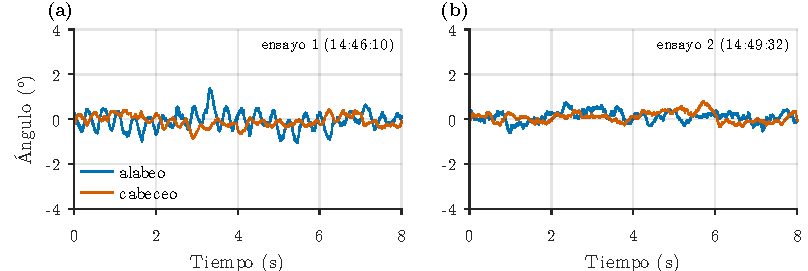
\includegraphics{figures/fig_drone_bench.pdf}
  \caption{Actitud del octocóptero sobre la rótula libre con colectivo de ralentí (\SI{1300}{\micro\second}), registro a bordo a 190--\SI{200}{\hertz}.}
  \label{fig:bench}
\end{figure}

\subsection{Campaña de vuelo en la guía}
\label{sec:flights}
El 20/11 se hicieron nueve vuelos en la guía con versiones sucesivas del firmware, con las LiPo cargadas a 12,4\,V en reposo al iniciar la sesión de la tarde. La Tabla~\ref{tab:flights} y la Fig.~\ref{fig:flights} los resumen.

\begin{itemize}
  \item \textbf{Vuelos 1--2.} Revelaron dos problemas: la saturación del acelerómetro por la vibración de los rotores (\SIrange{0.03}{2.2}{g}), que producía un falso corte por inclinación, y un giro real de guiñada del dron sobre la rótula. De ahí salieron el filtro de \SI{10}{\hertz} del acelerómetro y el lazo de guiñada.
  \item \textbf{Vuelos 3--6.} Despegaron, pero derivaron lentamente en cabeceo o alabeo hasta que el operador o el enclavamiento los detuvo. La deriva tenía un periodo de 5--\SI{10}{\second} y era la misma con ganancias completas (v5) y reducidas (v6). Esto apuntaba al límite de autoridad de par de la Sección~\ref{sec:authority}, cuya región de atracción era de solo 3--4$^\circ$, y no a las ganancias.
  \item \textbf{Vuelo 7} (v8, límite de velocidad angular más amplio). Primer vuelo estacionario estable: \SI{20}{\second} a 1725--\SI{1775}{\micro\second}, con alabeo RMS de \SI{0.55}{\degree} y cabeceo RMS de \SI{1.19}{\degree}. Se cortó durante el aterrizaje, cuando las ganancias volvieron a los valores de banco con el dron aún en el aire.
  \item \textbf{Vuelos 8--9} (v9, con histéresis). Volaron y aterrizaron sin corte. En el vuelo 9 el despegue necesitó \SI{1796}{\micro\second}, \SI{21}{\micro\second} más que en el vuelo 8, y el colectivo se subió hasta \SI{1816}{\micro\second}; tras \SI{48}{\second} de vuelo estacionario el cabeceo divergió hasta el límite de \SI{12}{\degree}. La saturación de la asignación no lo explica, porque \eqref{eq:taumax} aún da \SI{2.4}{\newton\metre}. Los candidatos son el modo lento poco amortiguado de la Sección~\ref{sec:attitude}, cuyo amortiguamiento depende de $k_T$, y la caída de tensión de la batería, que reduce $k_T$ con $V_{\mathrm{bus}}^2$: al final del vuelo 9 las LiPo habían entregado \SI{1.0}{\ampere\hour} cada una en la tarde (Sección~\ref{sec:bateria}). Más tarde, con 11,1\,V, el módulo ya no despegó.
\end{itemize}

\begin{table}[!htbp]
\centering
\caption{Campaña de vuelo en la guía (20/11/2026). Error RMS respecto a la horizontal, calculado mientras la orden media de motor superaba \SI{1650}{\micro\second}.}
\label{tab:flights}
\footnotesize
\setlength{\tabcolsep}{4pt}
\begin{tabularx}{\textwidth}{@{}clrrrrr>{\raggedright\arraybackslash}X@{}}
\toprule
Vuelo & FW & Col.\ máx. & $t$ & Alabeo & Cabeceo & Incl. & Resultado \\
 & & (\si{\micro\second}) & (\si{\second}) & RMS (°) & RMS (°) & máx.\ (°) & \\
\midrule
1 & v2 & 1625 & 0 & -- & -- & -- & corte por inclinación (vibración en el acelerómetro) \\
2 & v3 & 1475 & 0 & -- & -- & -- & corte por guiñada ($-20^\circ$) \\
3 & v4 & 1700 & 10,9 & 0,93 & 4,89 & 9,8 & parada del operador, deriva en cabeceo \\
4 & v5 & 1800 & 19,4 & 2,99 & 0,95 & 9,3 & parada del operador, oscilación lenta \\
5 & v6 & 1700 & 3,1 & 0,83 & 3,59 & 10,9 & corte por inclinación al despegar \\
6 & v6 & 1725 & 8,4 & 4,14 & 1,38 & 11,1 & corte por alabeo (videos IMG\_1867--1868) \\
7 & v8 & 1775 & 27,2 & 0,55 & 1,19 & 4,3 & estacionario \SI{20}{\second}; corte al aterrizar (video IMG\_1869) \\
8 & v9 & 1775 & 31,0 & 1,15 & 0,95 & 3,8 & estacionario y aterrizaje, sin corte \\
9 & v9 & 1816 & 62,0 & 1,73 & 1,70 & 10,8 & estacionario \SI{48}{\second}; corte por cabeceo \\
\bottomrule
\end{tabularx}
\end{table}

\begin{figure}[!htbp]
  \centering
  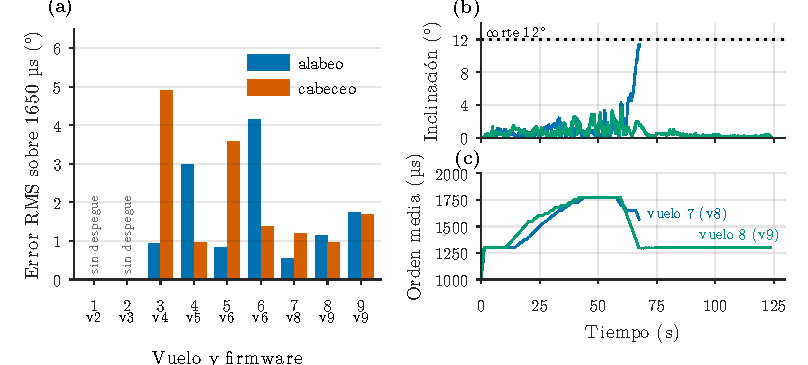
\includegraphics{figures/fig_flight_campaign.pdf}
  \caption{Campaña de vuelo en la guía. (a) Error RMS de alabeo y cabeceo por encima de \SI{1650}{\micro\second} en cada vuelo, con su versión de firmware. (b) Inclinación y (c) orden media de motor de los vuelos 7 (v8) y 8 (v9): el v8 se corta cuando las ganancias de vuelo se desactivan durante el aterrizaje, y el v9 aterriza con normalidad.}
  \label{fig:flights}
\end{figure}

\paragraph{Videos sincronizados con la telemetría}
Los tres videos del 20/11 (iPhone, 4K a \SI{120}{fps}) se sincronizaron con los registros por la hora de creación del archivo, que en el iPhone marca el inicio de la grabación, y por la hora del PC en cada línea del registro (Fig.~\ref{fig:video}). IMG\_1867 (15:10:11, \SI{11}{\second}) muestra el vuelo 6 mientras el colectivo sube de 1600 a \SI{1675}{\micro\second}. IMG\_1868 (15:10:26, \SI{4}{\second}) muestra su final: el alabeo pasa de $-6^\circ$ a $-11{,}1^\circ$ en \SI{1.3}{\second}, el firmware corta los motores y el módulo cae sobre la guía, lo que coincide con el registro con un desfase menor que \SI{1}{\second}. IMG\_1869 (15:23:32, \SI{13}{\second}) cae dentro del vuelo estacionario del vuelo 7, con el colectivo entre 1763 y \SI{1775}{\micro\second} y la inclinación entre 0,1 y 1,7$^\circ$. En los tres videos un operador acompaña con la mano el mástil de la cámara como medida de seguridad; el video no permite descartar un apoyo leve, que actuaría como una perturbación más sobre el lazo de actitud; las cifras de la Tabla~\ref{tab:flights} se toman tal como salen del registro.

\begin{figure}[!htbp]
  \centering
  \begin{subfigure}[b]{0.24\textwidth}\centering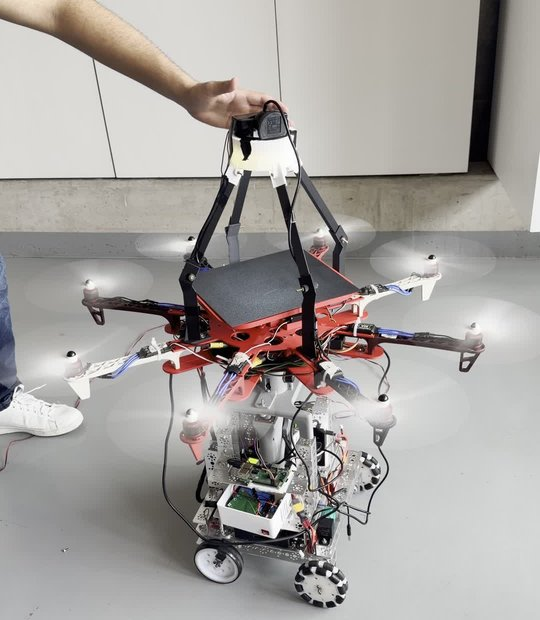
\includegraphics[width=\linewidth]{figures/video_a.jpg}\caption{Vuelo 6, \SI{1650}{\micro\second}.}\end{subfigure}\hfill
  \begin{subfigure}[b]{0.24\textwidth}\centering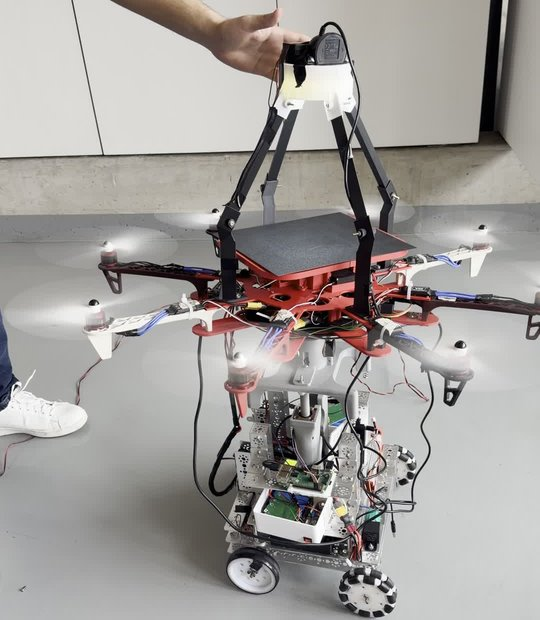
\includegraphics[width=\linewidth]{figures/video_b.jpg}\caption{Vuelo 6, \SI{1724}{\micro\second}.}\end{subfigure}\hfill
  \begin{subfigure}[b]{0.24\textwidth}\centering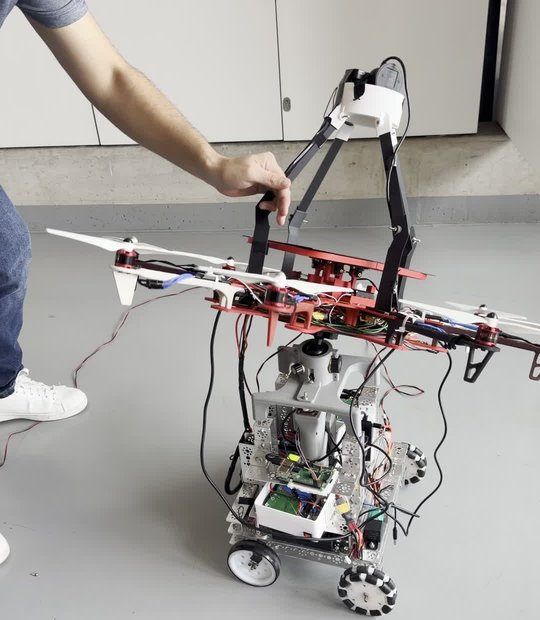
\includegraphics[width=\linewidth]{figures/video_c.jpg}\caption{Vuelo 6, tras el corte.}\end{subfigure}\hfill
  \begin{subfigure}[b]{0.24\textwidth}\centering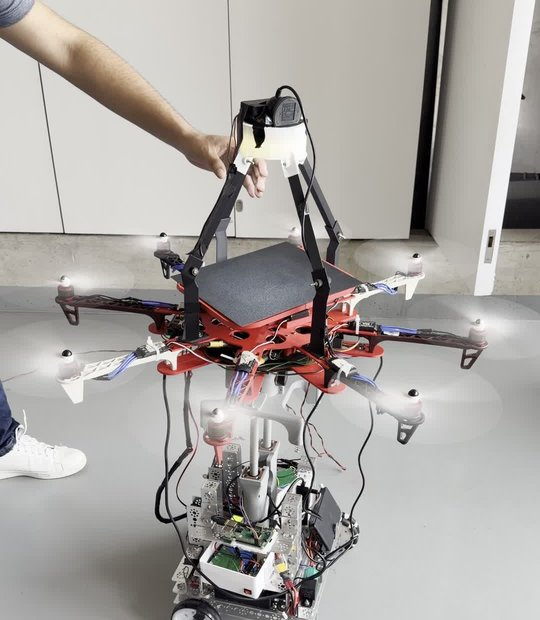
\includegraphics[width=\linewidth]{figures/video_d.jpg}\caption{Vuelo 7, \SI{1774}{\micro\second}.}\end{subfigure}
  \caption{Cuadros de los videos del 20/11 sincronizados con la telemetría: (a) IMG\_1867 a los \SI{6}{\second}, (b) IMG\_1868 a \SI{1}{\second}, (c) IMG\_1868 a \SI{3.2}{\second}, después del corte por alabeo de $-11{,}1^\circ$, con los motores detenidos y el módulo apoyado de lado, y (d) IMG\_1869 a los \SI{7}{\second}, en vuelo estacionario con 0,4--0,6$^\circ$ de inclinación. Las LiPo estaban cerca de 12,4\,V.}
  \label{fig:video}
\end{figure}

\paragraph{Comparación con el modelo de Isaac Lab}
Antes de los ensayos, el conjunto se modeló en Isaac Lab \cite{mittal2023} a partir del CAD, con la rótula y la guía (\SI{3.6}{\kilo\gram}, empuje limitado a \SI{6}{\newton} por motor). Allí se entrenaron y evaluaron una política PPO \cite{schulman2017} y un controlador clásico PI-D. La comparación muestra dos resultados distintos:
\begin{itemize}
  \item \textbf{Empuje.} El modelo predijo el vuelo estacionario en \SI{1899}{\micro\second} (\SI{4.41}{\newton} por motor); el conjunto real despegó 124--\SI{174}{\micro\second} antes, es decir, la ganancia real de empuje es 33--52\% mayor (Sección~\ref{sec:ident}). El modelo de empuje era conservador, y ese error, no el diseño del controlador, es lo que puso al lazo de actitud real dentro de la región estable de la Fig.~\ref{fig:dronestab}b. El simulador tampoco modelaba la tensión de la batería, que en el prototipo mueve el despegue más de \SI{100}{\micro\second} entre carga completa y descarga (Sección~\ref{sec:bateria}).
  \item \textbf{Actitud.} La inclinación RMS simulada fue \SI{0.02}{\degree} con PPO, \SI{0.04}{\degree} con el controlador clásico y \SI{0.12}{\degree} con perturbaciones; los valores medidos son 0,55--\SI{1.7}{\degree}. El modelo ignoraba cuatro efectos que dominaron el comportamiento real: la vibración de los rotores en la IMU, la excentricidad del centro de masa (\SI{9.5}{\milli\metre}), la saturación de la orden de velocidad angular, y el retraso y el retardo de actuación que, junto con el polo del péndulo invertido, ponen al lazo cerca del límite de la Sección~\ref{sec:limits_fund}. Los ocho motores simulados eran simétricos, mientras que la dispersión mediana real entre motores fue 50--\SI{90}{\micro\second}.
\end{itemize}

\subsection{\textit{Ball and plate} con la base fija y en movimiento}
La Fig.~\ref{fig:bp} y la Tabla~\ref{tab:bp} comparan cuatro condiciones:
\begin{enumerate}[label=(\alph*)]
  \item base quieta con el dron apagado (17/11, \SI{75}{\second});
  \item base quieta con los ocho rotores en ralentí y el lazo de actitud activo (17/11, \SI{469}{\second});
  \item robot avanzando en recta y girando en llano (18/11, cuatro recorridos, \SI{582}{\second});
  \item robot subiendo y bajando la rampa de \SI{10}{\degree} (18/11, seis recorridos, \SI{345}{\second}).
\end{enumerate}
Cada recorrido de (c) y (d) se emparejó con su video por la marca de tiempo del archivo de video.

\begin{table}[!htbp]
\centering
\caption{Error de la bola $|e|$ (distancia al centro del plato, en mm) en las cuatro condiciones. Diámetro de la bola \SI{27}{\milli\metre}; medio ancho del plato \SI{110}{\milli\metre}.}
\label{tab:bp}
\small
\begin{tabular}{@{}lrrrrr@{}}
\toprule
Condición & Muestras & Mediana & Media & P90 & P95 \\
\midrule
(a) base quieta, dron apagado & 13\,951 & 4,4 & 4,4 & 4,4 & 4,5 \\
(b) base quieta, dron en ralentí & 85\,219 & 18,9 & 23,1 & 39,9 & 60,4 \\
(c) en movimiento, llano & 95\,851 & 27,9 & 33,1 & 63,2 & 76,2 \\
(d) en movimiento, rampa de \SI{10}{\degree} & 62\,492 & 29,5 & 35,8 & 63,9 & 87,9 \\
\bottomrule
\end{tabular}
\end{table}

\begin{figure}[!htbp]
  \centering
  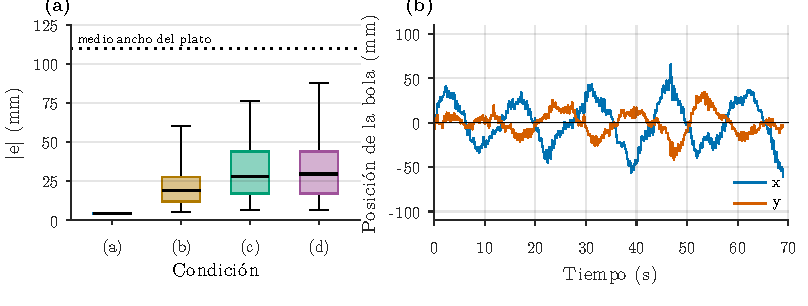
\includegraphics[width=\textwidth]{figures/fig_bp_results.pdf}
  \caption{Izquierda: distribución del error de la bola en las condiciones (a)--(d) de la Tabla~\ref{tab:bp} (caja: cuartiles; bigotes: percentiles 5 y 95). Derecha: posición de la bola durante un recorrido en la rampa (video \texttt{VID\_20261118\_165747}).}
  \label{fig:bp}
\end{figure}

\paragraph{Discusión}
\begin{itemize}
  \item \textbf{Dron apagado.} Con el dron apagado, el error es constante, \SI{4.4}{\milli\metre}: la bola se detiene dentro de la zona muerta de los servos. El ruido de visión está muy por debajo de ese valor.
  \item \textbf{Rotores en ralentí.} Encender los rotores multiplica por cuatro el error mediano (a \SI{18.9}{\milli\metre}). El modelo de propagación muestra que la actitud residual del octocóptero (dentro de \SI{0.4}{\degree}) explica solo unos \SI{2}{\milli\metre} RMS; el resto es una carga lenta que actúa directamente sobre la bola (flujo de los rotores, vibración y juego), concentrada por debajo de \SI{0.3}{\hertz} (Sección~\ref{sec:coupling}). Con las ganancias anteriores ($k_i=0.2$) la bola caía en menos de \SI{5}{\second}; tras subir la ganancia integral a 0,8 no hubo caídas en una prueba de \SI{20}{\second}, y se completó el ensayo de \SI{469}{\second} de la condición (b).
  \item \textbf{Base en movimiento.} Mover la base suma unos \SI{10}{\milli\metre} a la mediana y ensancha la cola (P95 de 76--\SI{88}{\milli\metre}), de acuerdo con el término de aceleración de la rótula de \eqref{eq:balllinx} y su amplificación a través del octocóptero (Fig.~\ref{fig:transm}c). La rampa es solo un poco peor que el llano: como predice \eqref{eq:tilt}, la rótula esférica absorbe la pendiente de \SI{10}{\degree} y el octocóptero mantiene nivelado el plato. Con la bandeja fija a la base, esa misma pendiente habría dejado a los servos con \SI{0.8}{\degree} de recorrido útil (Sección~\ref{sec:porquedron}).
  \item \textbf{Detección de la bola.} En los recorridos con la base en movimiento la bola se detectó el 61--100\% del tiempo. Los huecos incluyen caídas por el borde del plato, a menudo en los bordes de la rampa, donde el acelerómetro registró golpes de hasta \SI{1.95}{g}, y los momentos en que la bola se repuso con la mano.
\end{itemize}

\begin{figure}[!htbp]
  \centering
  \begin{subfigure}[b]{0.32\textwidth}\centering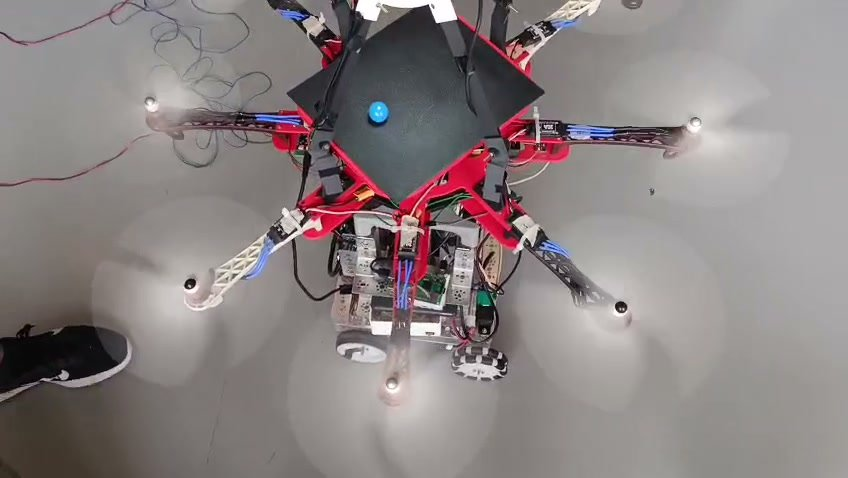
\includegraphics[width=\linewidth]{figures/photo_flat_turn.jpg}\caption{Giro en llano.}\end{subfigure}\hfill
  \begin{subfigure}[b]{0.32\textwidth}\centering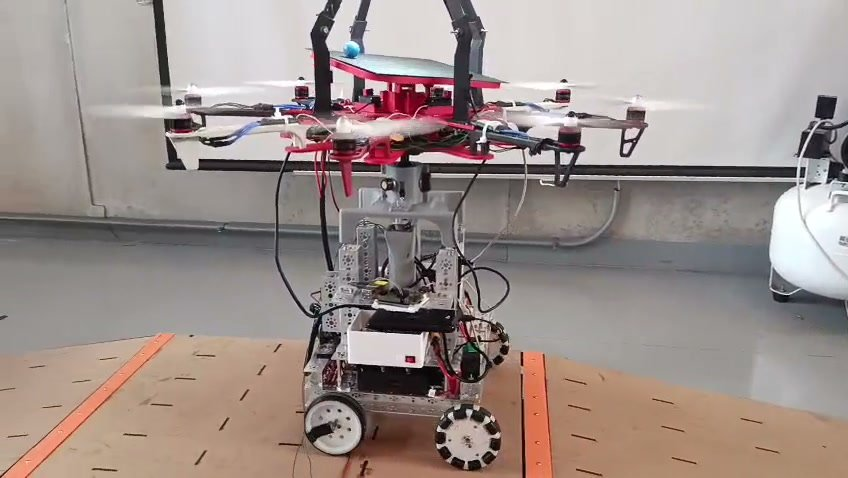
\includegraphics[width=\linewidth]{figures/photo_ramp_climb.jpg}\caption{Subiendo la rampa.}\end{subfigure}\hfill
  \begin{subfigure}[b]{0.32\textwidth}\centering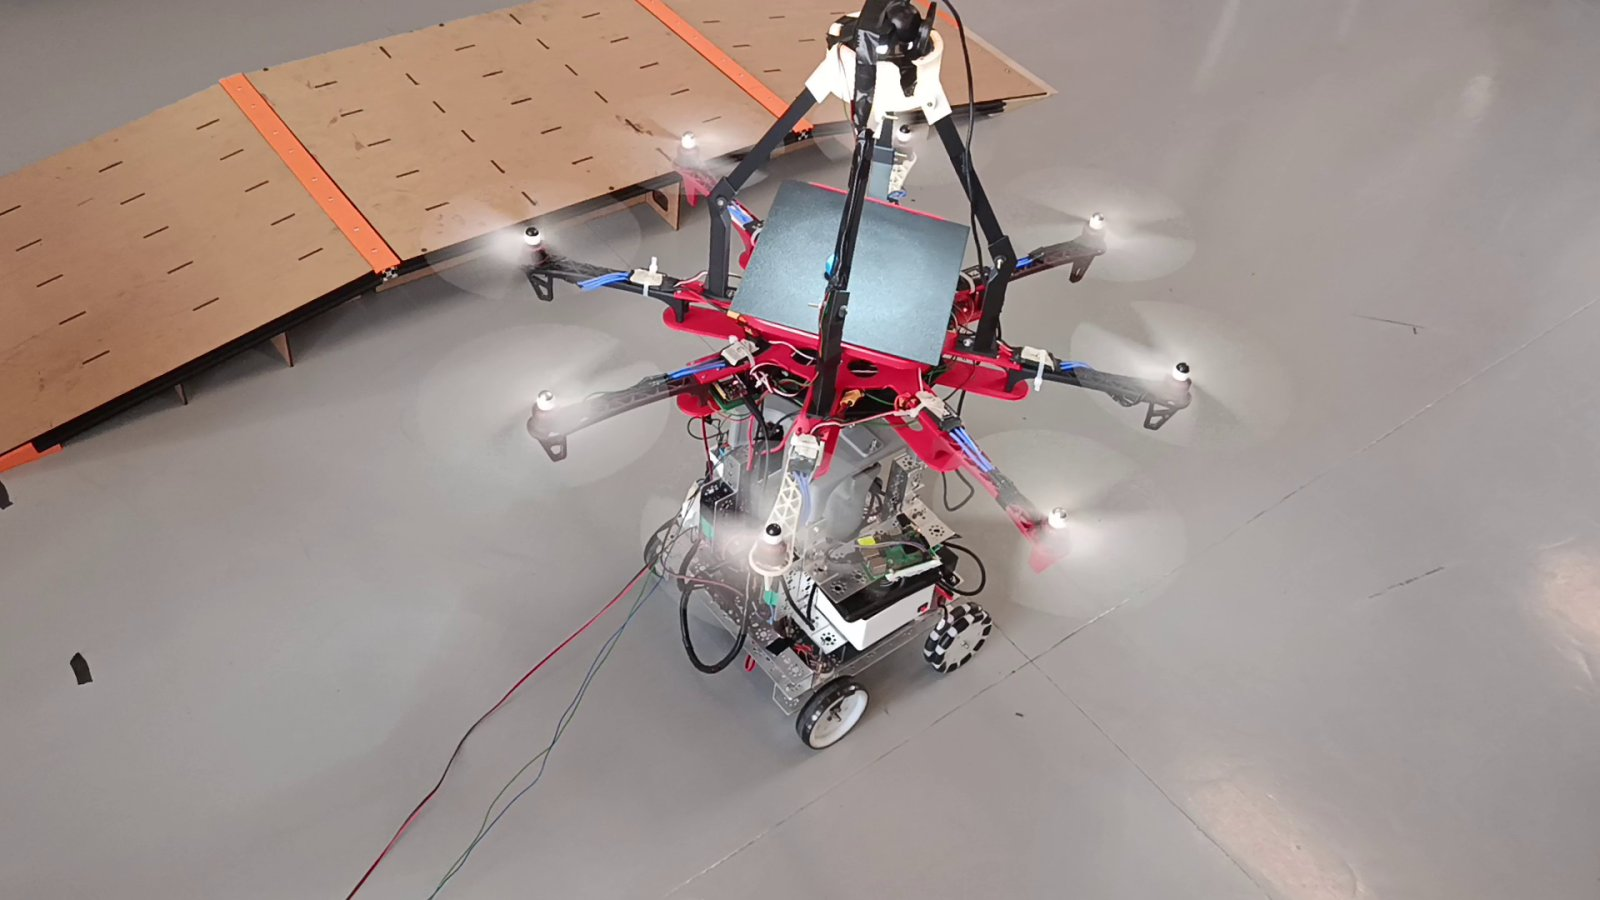
\includegraphics[width=\linewidth,trim=200 0 200 0,clip]{figures/photo_ramp_top.jpg}\caption{En lo alto de la rampa.}\end{subfigure}
  \caption{Pruebas integradas del 18/11/2026 con los rotores girando y la bola sobre el plato (cuadros de los videos de las pruebas).}
  \label{fig:tests}
\end{figure}

\subsection{Ensayos finales del robot completo (23/11)}
\label{sec:ensayos23}
El 23/11 se repitió el equilibrio de la bola sobre el robot completo: la base TETRIX con el octocóptero en la rótula y el \textit{ball and plate} encima, con el firmware v11 del dron (Secciones~\ref{sec:altura} y \ref{sec:metodologia}). Se registraron \textbf{13 ensayos} de equilibrio de entre 23 y \SI{122}{\second}, \SI{816}{\second} en total; en 10 de ellos los ocho rotores estaban encendidos (\SI{614}{\second}). Un ensayo empieza cuando el PID ve la bola dentro del plato y termina cuando la bola sale del plato o el operador lo detiene; se descartan sus primeros \SI{3}{\second}, en los que la bola se coloca a mano. La Tabla~\ref{tab:ensayos23} y la Fig.~\ref{fig:ensayos23} los resumen.

\paragraph{Origen de los datos y verificación} La Raspberry Pi registró la bola a \SI{187}{\hertz} (\texttt{registro\_20261123\_182316.csv}, 18:23--18:39), pero sus registros de antes y después de ese tramo no pudieron descargarse antes del informe. Para esos ensayos se recuperó la telemetría de las dos grabaciones de pantalla de la interfaz web (17:29 y 18:36): la página dibuja en vivo la bola sobre el mapa del plato y la inclinación del dron sobre sus círculos de 2, 5 y \SI{12}{\degree}, y el script \texttt{extraer\_de\_grabacion.py} mide la posición de esos puntos cuadro a cuadro (unos \SI{13}{\hertz}) con las escalas del código de la página. En los tramos que cubren a la vez la grabación y el registro de la Pi, la posición recuperada difiere de la registrada en 0,6 y \SI{1.4}{\milli\metre} de mediana (P90 de \SI{6.4}{\milli\metre}; 4007 muestras), muy por debajo de los errores que se reportan, así que ambas fuentes se tratan juntas. La recuperación no da los pulsos de los servos ni el colectivo del dron, pero sí el estado de la placa y de los motores.

\begin{table}[!htbp]
\centering
\caption{Ensayos de equilibrio de la bola sobre el robot completo (23/11/2026). Rot.: rotores encendidos. Fuente: registro de la Pi a \SI{187}{\hertz} o telemetría recuperada de la grabación de pantalla. Errores en mm; error relativo $e_{\mathrm{RMS}}/R_u$ en \%; efectividad: \% del tiempo con $e\le\SI{50}{\milli\metre}$. $^\ast$: ensayo completo, con la base cruzando la rampa (Tabla~\ref{tab:completos23}).}
\label{tab:ensayos23}
\footnotesize
\setlength{\tabcolsep}{3.5pt}
\begin{tabular}{@{}clrclrrrrrc@{}}
\toprule
Ens. & Hora & $t$ (s) & Rot. & Fuente & Mediana & RMS & P95 & Error rel. & Efect. & $\sigma_x$ / $\sigma_y$ \\
 & & & & & & & & & ($\le$\SI{50}{\milli\metre}) & \\
\midrule
01 & 17:30 & 27,0 & sí & video & 29,2 & 33,7 & 56,2 & 34,9 & 88,5 & 30,9 / 11,1 \\
02 & 17:32 & 98,5 & sí & video & 31,8 & 35,3 & 54,9 & 36,6 & 90,5 & 32,3 / 14,3 \\
03 & 17:45 & 122,3 & no & video & 31,5 & 35,0 & 55,7 & 36,3 & 92,1 & 31,2 / 15,7 \\
04 & 18:25 & 22,9 & no & Pi & 44,0 & 51,9 & 94,0 & 53,8 & 63,3 & 49,3 / 11,8 \\
05 & 18:26 & 95,9 & sí & Pi & 39,2 & 51,0 & 99,2 & 52,9 & 67,9 & 49,2 / 13,4 \\
06 & 18:33 & 57,0 & no & Pi & 31,3 & 45,1 & 97,1 & 46,7 & 77,5 & 41,6 / 14,9 \\
07 & 18:36 & 83,5 & sí & Pi & 33,5 & 38,3 & 63,9 & 39,7 & 81,2 & 35,5 / 14,4 \\
08 & 18:40 & 57,4 & sí & video & 42,8 & 46,1 & 72,8 & 47,7 & 65,4 & 40,8 / 20,9 \\
09 & 18:45 & 60,6 & sí & video & 35,1 & 47,3 & 86,5 & 49,0 & 70,2 & 43,4 / 18,8 \\
10$^\ast$ & 18:49 & 39,1 & sí & video & 33,2 & 41,4 & 67,8 & 42,9 & 71,7 & 38,4 / 12,7 \\
11$^\ast$ & 18:51 & 54,7 & sí & video & 42,0 & 48,0 & 82,9 & 49,7 & 67,1 & 38,3 / 28,1 \\
12$^\ast$ & 18:55 & 45,3 & sí & video & 33,4 & 42,6 & 77,4 & 44,1 & 75,7 & 37,2 / 19,6 \\
13$^\ast$ & 19:00 & 51,5 & sí & video & 33,5 & 41,0 & 73,2 & 42,5 & 77,3 & 38,4 / 14,4 \\
\midrule
\multicolumn{5}{@{}l}{Mediana de los 13 ensayos} & 33,5 & 42,6 & 73,2 & 44,1 & 75,7 & 38,3 / 14,4 \\
\bottomrule
\end{tabular}
\end{table}

\begin{figure}[!htbp]
  \centering
  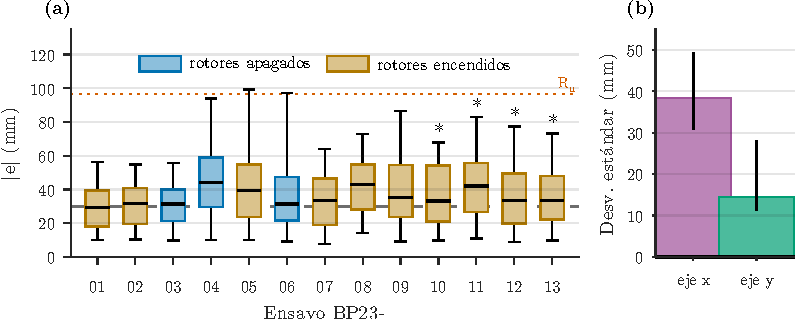
\includegraphics[width=\textwidth]{figures/fig_ensayos_23nov.pdf}
  \caption{Ensayos del 23/11 sobre el robot completo. (a) Distribución del error de la bola en cada ensayo; la línea discontinua marca \SI{30}{\milli\metre} y la punteada el radio útil del plato. (b) Desviación estándar de la posición en cada eje (barra: mediana de los 13 ensayos; bigotes: mínimo y máximo).}
  \label{fig:ensayos23}
\end{figure}

\paragraph{Resultados}
\begin{itemize}
  \item \textbf{Se registraron 13 tramos continuos de equilibrio de 23--\SI{122}{\second}}, con una mediana de 29--\SI{44}{\milli\metre} y el 63--92\% del tiempo a menos de \SI{50}{\milli\metre} del centro. Los tres ensayos de las 17:30--17:47 (BP23-01 a 03) son los mejores: mediana de 29--\SI{32}{\milli\metre} y 89--92\% del tiempo dentro de \SI{50}{\milli\metre}, con los rotores encendidos en dos de ellos. El error relativo cumple el criterio de $\le\SI{45}{\percent}$ de la Tabla~\ref{tab:metricas} en 7 de los 13 ensayos y queda entre 46 y \SI{54}{\percent} en los demás; la efectividad con la banda de \SI{30}{\milli\metre} (25--52\%) no alcanza el criterio de \SI{60}{\percent}.
  \item \textbf{Los rotores no degradan el equilibrio.} Con los rotores encendidos la inclinación del dron fue de 0,71--\SI{1.0}{\degree} RMS, y los ensayos con y sin rotores tienen la misma mediana (Fig.~\ref{fig:ensayos23}a). El dron mantuvo nivelado el plato durante los 10 ensayos sin ningún corte.
  \item \textbf{El error lo domina el eje $x$.} La dispersión en $x$ (31--\SI{49}{\milli\metre}) es 2,7 veces la de $y$ (11--\SI{28}{\milli\metre}) en todos los ensayos. En $x$ la bola oscila de lado a lado con un periodo de unos \SI{10}{\second} (Fig.~\ref{fig:bp23despegue}), y el servo $x$ trabaja con un sesgo medio de $+65$ a $+\SI{80}{\micro\second}$ sobre su neutro (\SI{1386}{\micro\second}) y llega a su tope de \SI{1612}{\micro\second}, mientras que el servo $y$ trabaja centrado. Es un desnivel del eje $x$ del plato montado sobre el dron: se come un tercio del recorrido del servo hacia ese lado, y la oscilación es el ciclo límite que produce la saturación con el integrador. La causa no es el dron, porque aparece igual con los rotores apagados. Volver a nivelar el neutro $x$ con el robot montado (rutina \texttt{/nivelar} de la Pi) es la corrección directa.
  \item \textbf{Comparación con el 17--18/11.} Con la base quieta y los rotores en ralentí, la mediana del 17/11 fue \SI{18.9}{\milli\metre} y la del 23/11 es 29--\SI{44}{\milli\metre}. Como la dispersión mediana del eje $y$ del 23/11 es \SI{14}{\milli\metre} y el exceso de error está en $x$, la diferencia se atribuye al desnivel de ese eje, que no se observó en las sesiones anteriores.
  \item \textbf{Fallo de alimentación de los servos (18:31--18:33).} En ese tramo los pulsos variaban entre 1200 y \SI{1580}{\micro\second}, pero la bola no se movió ni \SI{0.1}{\milli\metre}: la fuente de los servos estaba desconectada. Se identificó con una prueba directa de los servos y no se cuenta como ensayo.
\end{itemize}

\paragraph{Ensayos completos: la base cruzando la rampa con el dron y la bola} En cuatro de los ensayos (BP23-10 a 13) la base avanzó sobre la rampa de \SI{10}{\degree} mientras el dron, con los ocho rotores encendidos, nivelaba el plato y el PID mantenía la bola. El movimiento se confirma de dos formas independientes: la grabación de la pantalla de LabVIEW (18:48--19:10, Fig.~\ref{fig:completos23}d) muestra la orden \texttt{ADELANTE} con PWM del 25\% (23\% en la rueda derecha, por la compensación de 0,92) en esos intervalos, y los videos del celular \texttt{VID\_20261123\_184731}, \texttt{\_185130}, \texttt{\_185429}, \texttt{\_190032} y \texttt{\_190131}, cuya hora de inicio está en el nombre del archivo, muestran al robot subiendo y pasando los quiebres de la rampa (Fig.~\ref{fig:completos23}a--c). La Tabla~\ref{tab:completos23} separa el tramo con la base en movimiento.

\begin{table}[!htbp]
\centering
\caption{Ensayos completos del 23/11: base cruzando la rampa de \SI{10}{\degree}, dron con rotores encendidos y bola en equilibrio. Métricas de la bola calculadas solo mientras LabVIEW tenía la orden \texttt{ADELANTE}.}
\label{tab:completos23}
\small
\begin{tabular}{@{}lrrrrrr@{}}
\toprule
Ensayo & Base en & Mediana & P95 & Efect. & Incl.\ dron & Incl.\ dron \\
 & mov.\ (s) & (mm) & (mm) & ($\le$\SI{50}{\milli\metre}) & RMS (°) & máx.\ (°) \\
\midrule
BP23-10 & 22,9 & 29,6 & 53,7 & 91\,\% & 1,15 & 6,7 \\
BP23-11 & 29,5 & 34,5 & 74,6 & 81\,\% & 0,85 & 4,4 \\
BP23-12 & 18,2 & 30,7 & 52,9 & 89\,\% & 0,99 & 2,3 \\
BP23-13 & 19,0 & 30,6 & 74,7 & 80\,\% & 0,94 & 2,3 \\
\bottomrule
\end{tabular}
\end{table}

\begin{figure}[!htbp]
  \centering
  \begin{subfigure}[b]{0.32\textwidth}\centering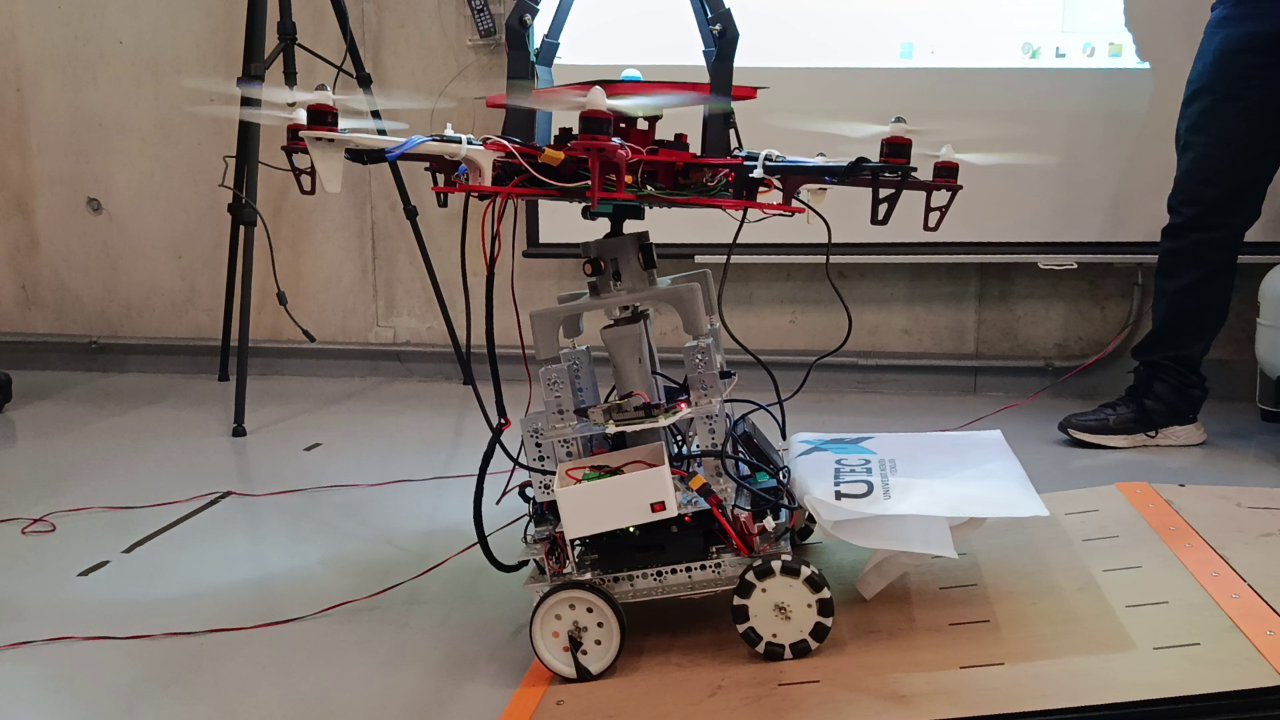
\includegraphics[width=\linewidth]{figures/ensayo23_a.jpg}\caption{BP23-12, 18:55:44.}\end{subfigure}\hfill
  \begin{subfigure}[b]{0.32\textwidth}\centering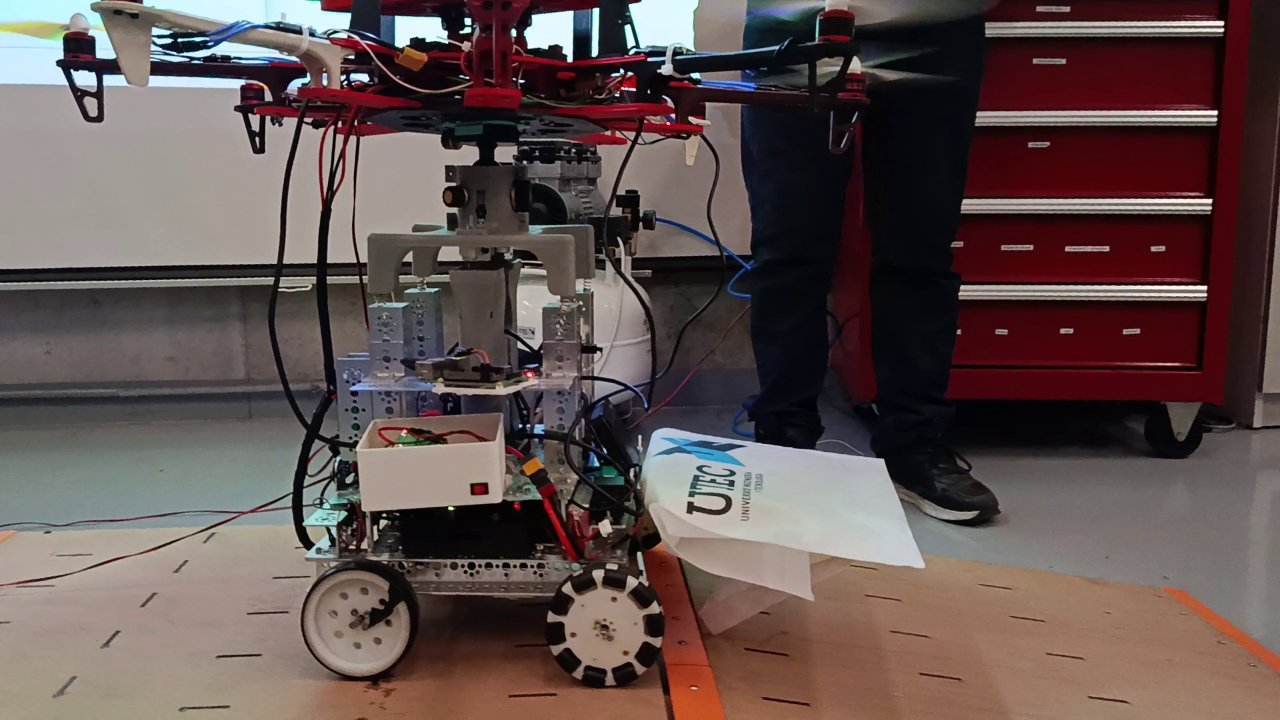
\includegraphics[width=\linewidth]{figures/ensayo23_b.jpg}\caption{BP23-12, 18:55:56.}\end{subfigure}\hfill
  \begin{subfigure}[b]{0.32\textwidth}\centering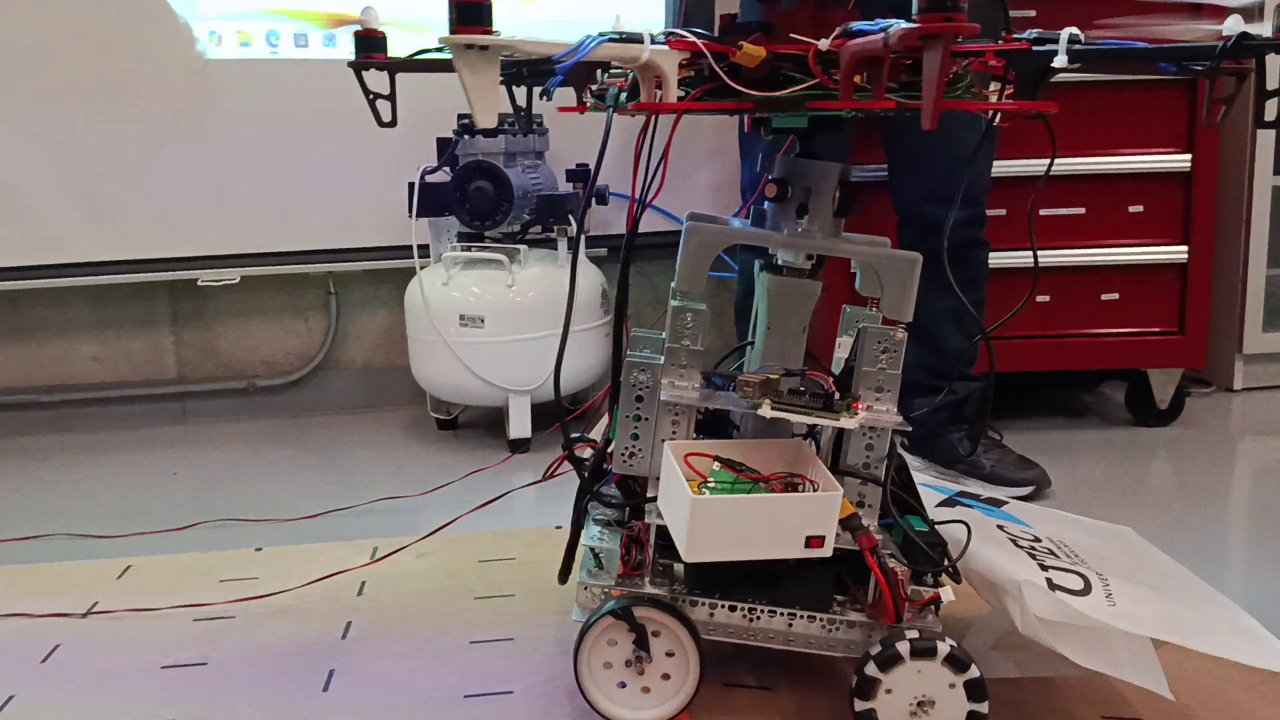
\includegraphics[width=\linewidth]{figures/ensayo23_c.jpg}\caption{BP23-13, 19:01:34.}\end{subfigure}\\[4pt]
  \begin{subfigure}[b]{0.7\textwidth}\centering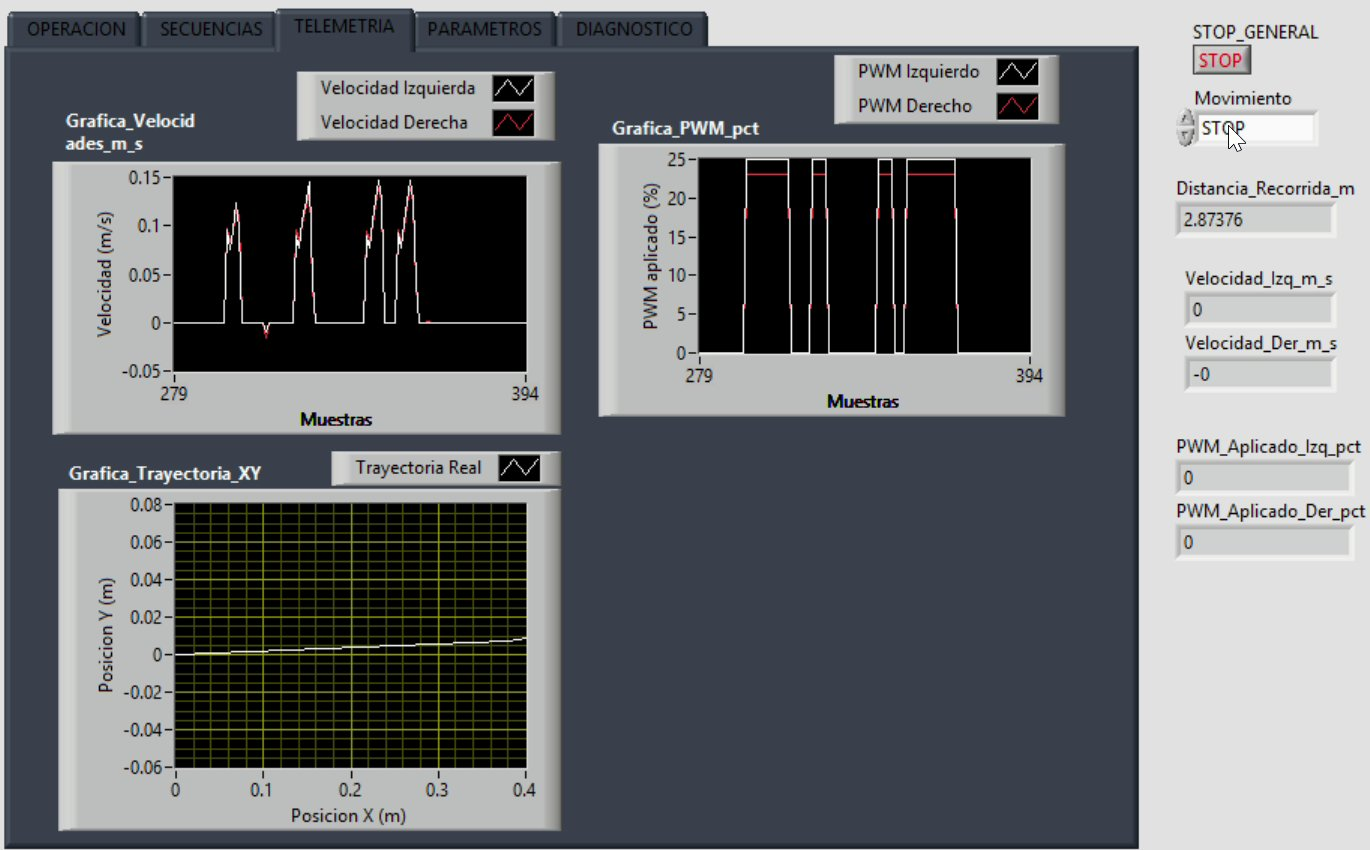
\includegraphics[width=\linewidth]{figures/ensayo23_labview.jpg}\caption{Telemetría de LabVIEW, 18:49:28.}\end{subfigure}
  \caption{Ensayos completos del 23/11. (a)--(c) El robot cruza la rampa con los ocho rotores girando y la bola sobre el plato (videos \texttt{VID\_20261123\_185429} y \texttt{\_190131}). (d) Panel de telemetría de la myRIO en el ensayo BP23-10: velocidad de cada rueda, PWM aplicado (25/23\,\%), trayectoria por odometría y orden \texttt{ADELANTE}.}
  \label{fig:completos23}
\end{figure}

Durante el cruce, la bola estuvo a una mediana de 30--\SI{35}{\milli\metre} del centro y el 80--91\% del tiempo dentro de \SI{50}{\milli\metre}, un error igual o menor que con la base quieta en los mismos ensayos (35--\SI{56}{\milli\metre}) y del mismo orden que los recorridos del 18/11 (mediana de \SI{29.5}{\milli\metre} en la rampa, Tabla~\ref{tab:bp}). La inclinación del dron fue de 0,85--\SI{1.15}{\degree} RMS, con picos de hasta \SI{6.7}{\degree} en los quiebres, y el firmware v11 no cortó los motores en ninguno, a diferencia de los recorridos del 18/11, que terminaron por los cortes de guiñada e inclinación del firmware de banco (Sección~\ref{sec:integrated}). La bola se mantuvo 18--\SI{30}{\second} de cruce en cada ensayo, del orden del cruce completo de la rampa medida (\SI{2.2}{\metre}; el modelo da \SI{19}{\second} con PWM del 25\%, Tabla~\ref{tab:modelval}); los cuatro ensayos terminaron durante el cruce, con la bola saliendo del plato en el tramo final (en BP23-13, al bajar el último quiebre, Fig.~\ref{fig:completos23}c), donde el 18/11 también se concentraban las caídas.

\paragraph{Base: velocidad y rectitud} La telemetría de LabVIEW registró las velocidades de rueda en los recorridos del 23/11. Con PWM del 25\% leyó 0,078--\SI{0.084}{\metre\per\second} en unos tramos y 0,124--\SI{0.134}{\metre\per\second} en otros; el modelo de \eqref{eq:vss} con la masa medida de \SI{10.4}{\kilo\gram} da \SI{0.078}{\metre\per\second} subiendo \SI{10}{\degree} y \SI{0.124}{\metre\per\second} en llano, así que los dos grupos de lecturas coinciden, dentro de un 8\%, con las dos predicciones; la telemetría no indica en qué tramo estaba la base, de modo que la asignación de cada grupo a un tramo es por cercanía. Con PWM del 40\% leyó entre 0,110 y \SI{0.222}{\metre\per\second}; el valor máximo queda un 8--10\% por encima de los \SI{0.201}{\metre\per\second} del modelo en llano. En un recorrido recto de \SI{2.16}{\metre} la odometría terminó con \SI{7.8}{\milli\metre} de desvío lateral (0,4\%) y \SI{-2.7}{\degree} de rumbo, con la compensación de 0,92 en la rueda derecha y el PI de rueda desactivado.

\paragraph{Despegue del dron con la bola encima} En el ensayo BP23-05 se ordenó flotar con la bola en equilibrio (Fig.~\ref{fig:bp23despegue}). El colectivo subió de 1300 a \SI{1750}{\micro\second} en \SI{25}{\second} sin que se perdiera la bola. A las 18:28:04 el módulo despegó en la guía: el láser pasó de 385 a \SI{499}{\milli\metre} (\SI{114}{\milli\metre} de subida) con la inclinación dentro de \SI{2.5}{\degree}, y aterrizó con la orden de aterrizar, sin ningún corte. Es el décimo vuelo en la guía (el primero con el firmware v11) y el primero con el plato y la bola encima. La bola, que medio segundo antes estaba en el centro ($x=\SI{-1}{\milli\metre}$), salió del plato en \SI{0.5}{\second}: el módulo no sube suave sino de golpe, porque la fricción de la guía lo retiene hasta que el empuje la vence, y el acelerómetro registró en ese instante de 0,28 a \SI{1.5}{g}. La aceleración vertical no la puede compensar el plato, así que la corrección está en el despegue: subir más lento cerca del empuje de despegue y enganchar el control de altura en cascada (Sección~\ref{sec:altura}) en cuanto el láser detecta la subida, para que el módulo no siga acelerando hacia arriba.

\begin{figure}[!htbp]
  \centering
  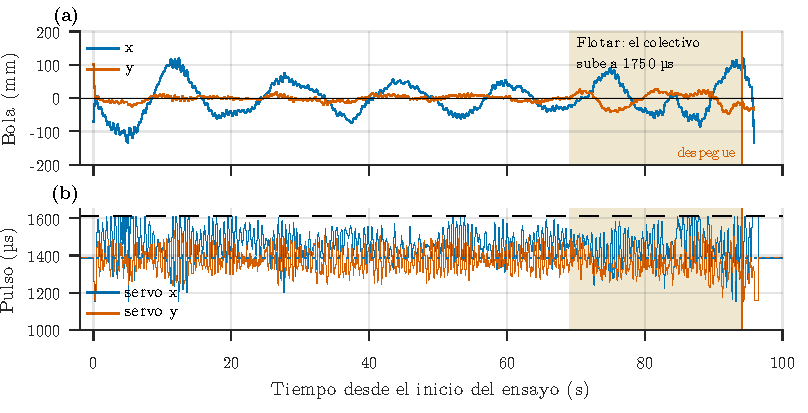
\includegraphics[width=\textwidth]{figures/fig_bp23_despegue.pdf}
  \caption{Ensayo BP23-05 (registro de la Pi a \SI{187}{\hertz}). Arriba: posición de la bola; abajo: pulsos de los servos, con el neutro del eje $x$ (punteado) y su tope (discontinuo). La franja marca la subida del colectivo hasta \SI{1750}{\micro\second} y la línea roja el despegue del dron, cuando la bola sale del plato. Se ve la oscilación lenta en $x$ y el sesgo del servo $x$ por encima de su neutro.}
  \label{fig:bp23despegue}
\end{figure}

\subsection{Base móvil y pruebas integradas}
\label{sec:integrated}
La Fig.~\ref{fig:tests} muestra cuadros de las pruebas integradas. La base, llevando el dron con los rotores girando y la bola sobre el plato, completó:
\begin{itemize}
  \item recorridos rectos y giros en llano;
  \item subidas y bajadas de la rampa de \SI{10}{\degree} en ambos sentidos, repetidas en varias pasadas (videos de las pruebas en la carpeta \texttt{videos/} del repositorio).
\end{itemize}
En los ocho recorridos integrados del 18/11 el dron usó el firmware de banco con el colectivo en \SI{1300}{\micro\second}, es decir, sin descargar peso ($f\approx0$), y los recorridos terminaron así:
\begin{itemize}
  \item cuatro por el corte de guiñada de \SI{20}{\degree}, porque el dron giraba con la base;
  \item tres por el corte de inclinación de \SI{12}{\degree}, medido en 12,0--\SI{12.2}{\degree} con velocidades angulares de hasta \SI{49}{\degree\per\second} al entrar a la rampa, lo que deja solo \SI{2}{\degree} de margen en una pendiente de \SI{10}{\degree};
  \item uno por el operador.
\end{itemize}
Estos eventos confirman el acoplamiento que predice \eqref{eq:pitchlin}: la aceleración de la rótula en los bordes de la rampa actúa sobre el módulo a través del término $-mh_ca_J$, y el modo lento de actitud lo amplifica (Fig.~\ref{fig:transm}b). El enlace UART entre la myRIO y la Pi se implementó en ambos lados y se verificó en la Pi con un puerto serie simulado: las tramas válidas se ejecutaron, las inválidas se rechazaron, se respetó la prioridad de la myRIO y se generó la telemetría de 6 campos. Después se probó con la myRIO conectada (Fig.~\ref{fig:uart}): la Pi envió por la UART la posición de la bola y el VI de la myRIO la recibió y la dibujó en tiempo real en su gráfica $x$--$y$, que recorre todo el plato ($\pm$\SI{150}{\milli\metre}) siguiendo los movimientos de la bola; el indicador de caracteres recibidos se encendió durante la prueba. En esa prueba las gráficas de alabeo y cabeceo del dron quedaron vacías, así que la telemetría del dron hacia la myRIO queda por verificar, y la sesión terminó con el aviso de LabVIEW de conexión perdida con la myRIO.

\begin{figure}[!htbp]
  \centering
  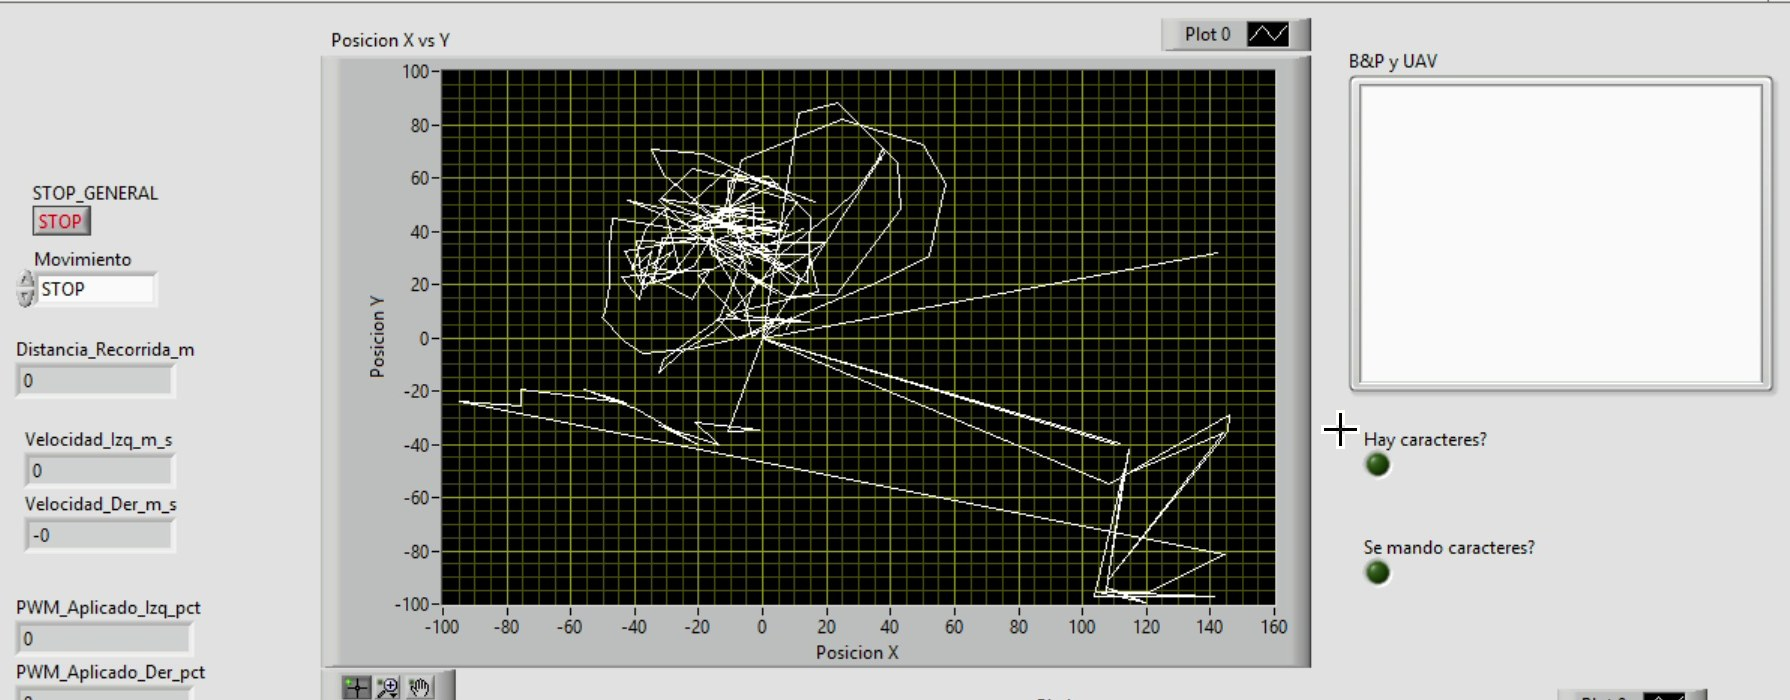
\includegraphics[width=0.9\textwidth]{figures/uart_myrio_bola.jpg}
  \caption{Prueba del enlace UART entre la Raspberry Pi y la myRIO: panel de LabVIEW con la posición de la bola recibida desde la Pi (gráfica $x$--$y$, en mm), la cadena recibida (\texttt{B\&P y UAV}) y los indicadores de recepción y envío.}
  \label{fig:uart}
\end{figure}

%% ---- TODO tras los ensayos finales del 23/11: llenar esta tabla (y descomentarla) ----
% \begin{table}[!htbp]\centering\small
% \caption{Ensayos finales de la base (odometria y video). Error = |posicion final - objetivo|.}
% \begin{tabular}{@{}lrrrr@{}}\toprule
% Ensayo & Objetivo & Medido (media $\pm$ de, $n$) & Error (\%) & Error mediano de la bola (mm) \\\midrule
% Traslacion, llano & 25 cm & & & \\
% Traslacion, llano & 50 cm & & & \\
% Traslacion, 10 grados & 25 cm & & & \\
% Giro sobre el punto medio del eje & 360 grados & & & \\
% Giro sobre una rueda & 360 grados & & & \\
% Subida de 10 grados con modo rampa (f = 0,5) & -- & & & \\
% \bottomrule\end{tabular}\end{table}

\subsection{Validación del modelo}
\label{sec:modelval}
La Tabla~\ref{tab:modelval} compara las predicciones del modelo de la Sección~\ref{sec:model} con las mediciones. Se marcan los parámetros identificados a partir de un conjunto de datos; las comparaciones de las demás filas usan datos que no se emplearon para construir el modelo.

\begin{small}
\setlength{\tabcolsep}{4pt}
\begin{longtable}{@{}>{\raggedright\arraybackslash}p{0.25\textwidth}>{\raggedright\arraybackslash}p{0.22\textwidth}>{\raggedright\arraybackslash}p{0.34\textwidth}>{\raggedright\arraybackslash}p{0.11\textwidth}@{}}
\caption{Predicciones del modelo frente a mediciones.}\label{tab:modelval}\\
\toprule
Magnitud & Modelo & Medición & Ec./Sec. \\
\midrule\endfirsthead
\toprule Magnitud & Modelo & Medición & Ec./Sec. \\ \midrule\endhead
Velocidad de la base, 15\%, llano & \SI{0.072}{\metre\per\second} & 0,06--\SI{0.08}{\metre\per\second} (telemetría de LabVIEW) & \eqref{eq:vss} \\
Velocidad de la base, 15\%, \SI{10}{\degree} & \SI{0.027}{\metre\per\second} & la rampa se subió más lento que el llano (videos) & \eqref{eq:vss} \\
Velocidad de la base, 25\%, llano / \SI{10}{\degree} (23/11) & 0,124 / \SI{0.078}{\metre\per\second} & 0,124--0,134 / 0,078--\SI{0.084}{\metre\per\second} (LabVIEW), error $\le\SI{8}{\percent}$ & \eqref{eq:vss} \\
Velocidad de la base, 40\%, llano (23/11) & \SI{0.201}{\metre\per\second} & máximo 0,217--\SI{0.222}{\metre\per\second} (+8 a +10\%) & \eqref{eq:vss} \\
Colectivo de vuelo estacionario & \SI{1899}{\micro\second} (mapa del firmware); \SI{1770}{\micro\second} (auditoría) & despegue a \SIrange{1725}{1775}{\micro\second} & \ref{sec:ident} \\
Despegue con batería descargada (vuelo 9) & \SI{1787}{\micro\second} (1758--1817) & \SI{1796}{\micro\second} & \eqref{eq:ureq} \\
Despegue con 11,1\,V en reposo & 1850--\SI{2000}{\micro\second}: no flota en régimen sostenido & no flotó & \eqref{eq:ureq} \\
Centro de masa del módulo & $h_c=\SI{0.10}{\metre}$ (CAD) & $h_c=0.14\pm\SI{0.06}{\metre}$, $\delta_x=9.5\pm\SI{1.8}{\milli\metre}$ (identificado) & \eqref{eq:cop} \\
Inclinación recuperable, límites v4--v7 & $\theta^\ast=$ 2,8--\SI{3.8}{\degree} & los vuelos 3--6 derivaron hasta el enclavamiento de \SI{12}{\degree} & \eqref{eq:thetastar} \\
Inclinación recuperable, límites v8--v9 & $\theta^\ast=$ 16--\SI{19}{\degree} & los vuelos 7--9 se mantuvieron 20--\SI{48}{\second} & \eqref{eq:thetastar} \\
Modo lento de actitud en vuelo estacionario & 0,20--\SI{0.30}{\hertz}, $\zeta=$ 0,24--0,42 & picos espectrales en 0,15--\SI{0.23}{\hertz} & \ref{sec:attitude} \\
Lazo de la bola, ganancia derivativa & estable 4,5 e inestable 6 para $K_{b,\mathrm{eff}}=$ 3,5--4,9 & 4,5 estable, 6 inestable (banco) & \ref{sec:ballcontrol} \\
Ganancia de planta de la bola & 6,0 (CAD); 3,5--4,9 (inferida) & 2,5 / 4,9 ($x$/$y$, regresión, $R^2\le0.45$) & \eqref{eq:balltf} \\
Error de la bola debido a la actitud, rotores encendidos & 1,7--\SI{2.1}{\milli\metre} RMS & 16--\SI{21}{\milli\metre} RMS (dominado por $D_b$) & \eqref{eq:propag} \\
Error de la bola, base quieta frente a en movimiento & aumento por las aceleraciones de la base & mediana +9 a \SI{11}{\milli\metre} & \eqref{eq:balllinx} \\
Pendiente de vuelco estático (módulo trabado) & CM del CAD: $x_G=\SI{81}{\milli\metre}$ & \SI{21.5}{\degree} al subir y \SI{30.5}{\degree} al bajar (23/11), es decir $x_G=\SI{88}{\milli\metre}$: el CAD difiere un \SI{8}{\percent} & \eqref{eq:tip} \\
Recorrido de la guía & \SI{77}{\milli\metre} (CAD) & unos \SI{140}{\milli\metre} (medido) & Tabla~\ref{tab:params} \\
Rango de la rótula frente a los quiebres de la rampa & necesario $>\SI{10}{\degree}$ & 35--\SI{53}{\degree} según la dirección & Sec.~\ref{sec:metodologia} \\
Altura con láser calibrado y Kalman & \SI{330}{\milli\metre} (regla) & 317--\SI{334}{\milli\metre} (error $\le\SI{4}{\percent}$) & \eqref{eq:kfz} \\
Control de altura en cascada & 4--\SI{12}{\milli\metre} pico a pico (simulación) & no ensayado en vuelo; el láser con Kalman registró el despegue del vuelo 10 (\SI{114}{\milli\metre} de subida) & \eqref{eq:cascada} \\
Ciclo de rampa (\SI{0.7}{\metre} a \SI{10}{\degree} + \SI{0.8}{\metre} + \SI{0.7}{\metre}), PWM del \SI{15}{\percent} & \SI{41}{\second} en ralentí; \SI{37}{\second} en modo rampa & pendiente (cronómetro) & \eqref{eq:vss}, \eqref{eq:descarga} \\
Cruce de la rampa con PWM del \SI{25}{\percent} (23/11) & \SI{19}{\second} & orden \texttt{ADELANTE} de \SI{25.5}{\second} en BP23-12; bola mantenida 18--\SI{30}{\second} de cruce & \eqref{eq:vss}, \eqref{eq:descarga} \\
\bottomrule
\end{longtable}
\end{small}

El modelo reproduce todas las magnitudes para las que existe una medición, en la mayoría de los casos dentro de la incertidumbre de los parámetros. Su principal discrepancia abierta es el tamaño de la perturbación directa sobre la bola, $D_b$, que el modelo trata como una entrada externa; cuantificar el flujo de los rotores sobre el plato es el siguiente experimento natural. Las predicciones de descarga de peso en la rampa aún no tienen medición.

\subsection{Cumplimiento de los requisitos y limitaciones}
\label{sec:requirements}
\label{sec:limits}
La Tabla~\ref{tab:req} compara los resultados con los escenarios de validación de la guía del curso.

\begin{table}[!htbp]
\centering
\caption{Estado de los escenarios de validación de la guía del proyecto.}
\label{tab:req}
\footnotesize
\renewcommand{\arraystretch}{1.1}
\begin{tabularx}{\textwidth}{@{}>{\raggedright\arraybackslash}p{0.34\textwidth}>{\raggedright\arraybackslash}X>{\raggedright\arraybackslash}p{0.17\textwidth}@{}}
\toprule
Escenario & Evidencia & Estado \\
\midrule
Traslación y giro de la base (llano, \SI{10}{\degree}) & rampa subida y bajada en ambos sentidos; velocidades del 23/11 dentro de un 8--10\% del modelo; desvío lateral del 0,4\% en \SI{2.16}{\metre}; modos de odometría para \SI{25}{\centi\metre}, \SI{50}{\centi\metre} y \SI{360}{\degree} implementados & cumplido en traslación; giro sin métrica final \\
Base en pendiente de \SI{20}{\degree} & no ensayada; sin empuje el vuelco estático medido es \SI{21.5}{\degree} (margen de \SI{0.26}{\metre\per\second\squared} en \SI{20}{\degree}); con el modo rampa ($f=0.35$--0,55) el margen pasa a 0,72--\SI{0.98}{\metre\per\second\squared} (Sección~\ref{sec:porquedron}) & no cumplido; viable con modo rampa, por validar \\
Estimación de la plataforma y de la bola & detección a \SI{187}{fps} en todo el plato; calibración por homografía & cumplido \\
Equilibrio con la base fija & mediana 4,4 / \SI{18.9}{\milli\metre} (dron apagado / encendido, 17/11), sin caídas; 13 tramos continuos de 23--\SI{122}{\second} el 23/11 (\SI{816}{\second}, 10 con rotores), mediana 29--\SI{44}{\milli\metre} (Tabla~\ref{tab:ensayos23}) & cumplido \\
Equilibrio durante la traslación (llano, \SI{10}{\degree}) & mediana 27,9 / \SI{29.5}{\milli\metre} (18/11), P95 por debajo del medio ancho del plato; cuatro ensayos completos del 23/11 cruzando la rampa con los rotores encendidos: mediana 30--\SI{35}{\milli\metre}, 18--\SI{30}{\second} de cruce, sin cortes del dron (Tabla~\ref{tab:completos23}) & cumplido, con caídas en el tramo final de la rampa \\
Equilibrio durante el giro & recorridos con giros incluidos en la condición (c) & cumplido en parte (cortes por guiñada) \\
Etapa intermedia (octocóptero) & RMS en banco $<$\SI{0.4}{\degree}; tres vuelos estacionarios en la guía de \SIrange{20}{48}{\second} (vuelos 7--9); 0,71--\SI{1.0}{\degree} RMS con rotores y la bandeja encima (23/11); despegue y aterrizaje sin corte con la bola encima (vuelo 10, v11) & cumplido en la guía \\
Interfaz y registro & interfaz web, panel de LabVIEW, registros CSV a la tasa de la cámara y del dron & cumplido \\
\bottomrule
\end{tabularx}
\end{table}

Las limitaciones principales son:
\begin{enumerate}[label=(\roman*)]
  \item \textbf{Cortes en los recorridos integrados y funciones pendientes de v11.} En los recorridos del 18/11 el firmware de banco cortó por guiñada (\SI{20}{\degree}) y por inclinación (\SI{12}{\degree}). El firmware v11 resolvió el corte de guiñada en ralentí ($\le\SI{1400}{\micro\second}$) con la ventana deslizante de $\pm\SI{20}{\degree}$ y tope de seguridad de \SI{120}{\degree\per\second}, lo que permitió completar los cuatro cruces de rampa del 23/11 sin cortes. Quedan pendientes escalar el límite de inclinación de \SI{12}{\degree} con la pendiente y validar el seguimiento activo de guiñada (\texttt{yb}) desde la myRIO en giros completos de \SI{360}{\degree}.
  \item \textbf{Batería sin medición.} El firmware no lee la tensión de las LiPo, y el margen de empuje cae con su cuadrado: el vuelo sostenido útil es de 3--\SI{7}{\minute} por par de baterías, y con 11,1\,V en reposo el módulo ya no despega por debajo del límite sostenido (Sección~\ref{sec:bateria}).
  \item \textbf{Ensayos pendientes del protocolo (trabajo futuro).} No se ejecutaron en la campaña del 23/11 la descarga de peso en rampa ($f=0.5$; los recorridos se hicieron en ralentí), el ensayo comparativo D (dron trabado C2 frente a dron libre C3), las repeticiones con cinta de \SI{25}{\centi\metre}, \SI{50}{\centi\metre} y giros de \SI{360}{\degree} (E1), el barrido sinusoidal del plato (E2) ni las pruebas de recuperación desde 2 y \SI{5}{\centi\metre} (E3).
  \item \textbf{Centro de masa y margen de autoridad.} La excentricidad de \SI{9.5}{\milli\metre} exige \SI{0.31}{\newton\metre} permanentes, y la altura del centro de masa sobre la rótula ($h_c\approx\SI{0.14}{\metre}$) hace pequeña la rigidez neta del lazo de actitud (Sección~\ref{sec:attitude}).
  \item \textbf{Mapa de empuje.} El mapa no se identificó con una celda de carga; los datos de despegue indican que $k_F$ es 33--52\% mayor que el supuesto, y su forma con colectivo alto es desconocida.
  \item \textbf{Alimentación.} El BMS original de servos y bobinas falló y en parte de los ensayos se usó una fuente de banco; GPIO5 y GPIO14 emiten pulsos al arrancar el ESP32, lo que obliga a energizar los ESC después del arranque.
  \item \textbf{Visión.} La bola se detecta por color, así que la iluminación debe controlarse.
  \item \textbf{Altura de la rótula.} El centro de masa del módulo está sobre la rótula, así que el módulo es un péndulo invertido ($h_c=0.14\pm\SI{0.06}{\metre}$, polo inestable de \SI{6.1}{\radian\per\second}) y el control de actitud opera cerca del límite por retardo $p\theta_e\approx0.5$. Bajar el centro de masa por debajo de la rótula lo haría pasivamente estable.
  \item \textbf{Parámetros del modelo.} La inercia $\vect J$, la distribución de masas de la base y la resistencia interna de las LiPo son estimaciones basadas en el CAD, en pruebas o en valores típicos, y el retardo del servo se infirió y no se midió; un banco de empuje con celda de carga, un ensayo de péndulo bifilar para la inercia, un ensayo de escalón del servo y una medición de la caída de tensión bajo carga cerrarían estas brechas.
\end{enumerate}
          % 8. Validacion y caracterizacion
%% ======================================================================
%% 10_conclusions.tex -- 9. Conclusiones
%% ======================================================================
\section{Conclusiones}
\label{sec:conclusions}
AeroTray muestra que tres lazos de equilibrio independientes pueden apilarse sobre una base móvil con hardware de bajo costo, y que la propagación de la perturbación de la base a través de ellos puede tanto medirse con registros sincronizados como predecirse con un modelo de primeros principios. El modelo, verificado simbólicamente y parametrizado con el ensamble CAD, las hojas de datos y los registros, lleva a seis conclusiones que los experimentos confirman.

(i) El módulo aéreo es un péndulo invertido sobre un pivote acelerado cuyo centro de masa, identificado con telemetría de vuelo estacionario, está $0{,}14\pm\SI{0.06}{\metre}$ sobre la rótula y \SI{9.5}{\milli\metre} hacia M8. (ii) El lazo de actitud funciona solo porque la rigidez proporcional supera a la gravitatoria por un margen pequeño, que proporcionó la ganancia de empuje subestimada; ese margen explica el modo lento de actitud observado en vuelo estacionario. (iii) Las divergencias lentas de los primeros vuelos eran un problema de autoridad de par, con una región de atracción de solo 3--4$^\circ$, y se resolvieron ampliando el límite de la velocidad angular pedida, no reajustando ganancias. (iv) El lazo de la bola está limitado por su retardo y por un cero en el semiplano derecho que introduce la altura de la bola sobre el pivote del plato, que juntos explican el techo de la ganancia derivativa; la ganancia efectiva de la planta es alrededor del 70\% de la del CAD por el juego del mecanismo. (v) La rótula pasiva elimina la pendiente de la dinámica de la bola, los giros son benignos, y el error residual de la bola con los rotores girando lo domina una carga aerodinámica y vibratoria directa y lentamente variable, no el movimiento de actitud del octocóptero.

(vi) El dron se justifica en la rampa por dos razones cuantificadas. Al nivelarse, desacopla la pendiente del plato y deja libre entre el 84 y el 95\% del recorrido de los servos, que con la bandeja fija se agotaría en una pendiente de \SI{11}{\degree}. Al sostener parte de su peso, actúa como un lastre ajustable que baja el centro de masa: con la mitad del peso del módulo en los rotores, la pendiente de vuelco al subir pasa de \SI{21.5}{\degree} (medida con el robot completo de \SI{10.4}{\kilo\gram}) a \SI{27.7}{\degree} (prevista), al bajar de \SI{30.5}{\degree} a \SI{38.2}{\degree} (prevista), y el margen de aceleración en \SI{20}{\degree} se multiplica por 3,5. El dron no debe flotar en la rampa, sino trabajar en una ventana del 35--55\% de su peso, a un costo de 2--5\% de batería por minuto. El margen de empuje para flotar, en cambio, depende del cuadrado de la tensión de las LiPo: con 12,4\,V el módulo despega a 1725--\SI{1775}{\micro\second}, y con 11,1\,V necesitaría 1850--\SI{2000}{\micro\second}, lo que explica que dejara de flotar y limita el vuelo útil a 3--\SI{7}{\minute} por par de baterías.

Experimentalmente, el firmware final mantiene el módulo de \SI{3.6}{\kilo\gram} en la guía con 0,55--\SI{1.7}{\degree} de error RMS de actitud, y el controlador de la bola la mantiene a una mediana de 19--\SI{30}{\milli\metre} del centro con la base quieta, en llano y en una rampa de \SI{10}{\degree}. En los ensayos finales sobre el robot completo (23/11) se registraron 13 ensayos de equilibrio de 23--\SI{122}{\second} (\SI{816}{\second} totales; mediana de 29--\SI{44}{\milli\metre}), con los rotores encendidos en 10 de ellos y el dron nivelado a 0,71--\SI{1.0}{\degree} RMS; en cuatro ensayos completos la base cruzó la rampa de \SI{10}{\degree} con los rotores encendidos y la bola en equilibrio durante 18--\SI{30}{\second} (mediana de 30--\SI{35}{\milli\metre}, dron a 0,85--\SI{1.15}{\degree} RMS sin ningún corte, con la bola saliendo del plato en el tramo final), y el módulo también despegó y aterrizó en la guía con la bandeja encima (la bola salió al despegar). La velocidad de la base medida ese día coincide con el modelo dentro de un 8--10\%. Dos correcciones concretas salen de esos ensayos: volver a nivelar el neutro del eje $x$ del plato, que concentra el error, y suavizar el despegue en la guía, cuyo salto por fricción es lo que hizo caer la bola al despegar. El modelo también señala los siguientes pasos con mayor beneficio esperado: medir la tensión de las baterías y compensar el colectivo, ensayar el modo rampa, bajar el centro de masa del módulo por debajo de la rótula, acortar el retardo del lazo de la bola, proteger el plato del flujo de los rotores y suavizar las referencias de la base. Todos los archivos de diseño, el código, los scripts de análisis, los videos y los datos crudos se publican para que estos experimentos puedan reproducirse y ampliarse, por ejemplo con la prealimentación de inclinación ya implementada o con controladores entrenados sobre el modelo publicado.
         % 9. Conclusiones
%% ======================================================================
%% 11_declarations.tex -- etica, CRediT, conflicto de intereses, declaracion de IA, agradecimientos, biografias
%% ======================================================================
\section*{Declaraciones éticas}
Este trabajo no involucró participantes humanos, experimentos con animales ni datos recogidos de redes sociales.

\section*{Contribución de los autores (CRediT)}
\textbf{Sebastián Rejas Córdova:} Conceptualización, Metodología, Investigación (integración y verificación), Validación, Redacción -- revisión y edición.
\textbf{George Henry Ramos Astuhuamán:} Software (supervisor en la Raspberry Pi, visión, firmware del octocóptero y de la ESP32-S3, interfaz web), Metodología (modelo cinemático y dinámico, identificación), Análisis formal, Curación de datos, Visualización, Redacción -- borrador original.
\textbf{Johan Nireo Naupay Fabián:} Metodología, Recursos (diseño y auditoría del sistema de alimentación), Investigación (integración), Redacción -- revisión y edición.
\textbf{Hideky Edu Garnique Pisfil:} Investigación (validación en llano), Software (interfaz de usuario), Visualización, Redacción -- revisión y edición.
\textbf{Diego André Miranda Zamora:} Software (control de la base en LabVIEW y enlace UART myRIO--Pi), Investigación (validación en la rampa), Redacción -- revisión y edición.

\section*{Declaración de conflicto de intereses}
Los autores declaran que no tienen intereses financieros en competencia ni relaciones personales conocidas que pudieran haber influido en el trabajo presentado en este artículo.

\paragraph{Financiamiento}
\tocheck{Este trabajo no recibió financiamiento externo; se usaron equipos del laboratorio de UTEC.}

\section*{Declaración sobre el uso de IA generativa y tecnologías asistidas por IA en la redacción}
Durante la preparación de este manuscrito, los autores emplearon de forma puntual las herramientas de inteligencia artificial Claude (Anthropic) y Gemini (Google) únicamente como apoyo en tareas específicas:
\begin{itemize}
  \item revisión y búsqueda preliminar de literatura técnica y antecedentes;
  \item corrección gramatical, ortográfica y de estilo del manuscrito;
  \item depuración puntual de errores en el código desarrollado por el equipo.
\end{itemize}
El diseño mecánico y eléctrico, el modelado matemático, la construcción del prototipo, la programación de los subsistemas, la ejecución de los ensayos y el análisis de resultados fueron realizados por los autores. Después de utilizar estas herramientas, los autores revisaron, editaron y verificaron el contenido frente al código fuente y los registros experimentales, y asumen la plena responsabilidad por el contenido de la publicación.

\section*{Agradecimientos}
Los autores agradecen a los profesores del curso MT5001 Diseño de Sistemas Mecatrónicos (Elvis Jara y Rodrigo Magallanes) y al personal de los laboratorios de la UTEC por el equipamiento (myRIO, kit TETRIX y fuentes de banco) y su orientación.

\section*{Biografías}
\noindent\textbf{Sebastián Rejas Córdova} es estudiante de pregrado de Ingeniería Mecatrónica en la UTEC (Lima, Perú). Sus intereses son el diseño mecánico y la integración de sistemas de robots móviles.

\noindent\textbf{George Henry Ramos Astuhuamán} es estudiante de pregrado de Ingeniería Mecatrónica en la UTEC. Sus intereses son el control embebido, la visión por computadora y la robótica aérea.

\noindent\textbf{Johan Nireo Naupay Fabián} es estudiante de pregrado de Ingeniería Mecatrónica en la UTEC. Sus intereses son la electrónica de potencia y los sistemas de energía para robots.

\noindent\textbf{Hideky Edu Garnique Pisfil} es estudiante de pregrado de Ingeniería Mecatrónica en la UTEC. Sus intereses son las interfaces humano--máquina y la validación experimental.

\noindent\textbf{Diego André Miranda Zamora} es estudiante de pregrado de Ingeniería Mecatrónica en la UTEC. Sus intereses son el control en tiempo real con hardware de NI y la comunicación entre robots.
        % etica, CRediT, IA, agradecimientos, biografias

\appendix
%% ======================================================================
%% A_derivations.tex -- Apendice A: deducciones y su verificacion simbolica
%% ======================================================================
\section{Deducciones y verificación}
\label{app:derivations}

\subsection{Bola sobre un plato que acelera y rota}
Todos los vectores se escriben en $\{P\}$, que rota con $\vect\Omega$ y cuyo origen $G$ tiene aceleración absoluta $\vect a_G$. Con $\vect\rho=[x_b,y_b,\varepsilon]\T$ y la velocidad relativa $\dot{\vect\rho}=[\dot x_b,\dot y_b,0]\T$, la aceleración absoluta del centro de la bola es
\begin{equation}
  \vect a_b=\vect a_G+\dot{\vect\Omega}\times\vect\rho+\vect\Omega\times(\vect\Omega\times\vect\rho)+2\,\vect\Omega\times\dot{\vect\rho}+\ddot{\vect\rho}.
  \tag{A.1}
\end{equation}
El punto de contacto de la bola es $\vect\rho-r_b\ez$. Igualando su velocidad, $\vect v_G+\vect\Omega\times\vect\rho+\dot{\vect\rho}+\vect\omega_b\times(-r_b\ez)$, con la del punto del plato que toca, $\vect v_G+\vect\Omega\times(\vect\rho-r_b\ez)$, se obtiene la restricción de rodadura $\dot{\vect\rho}=r_b\,\vect w\times\ez$ con $\vect w=\vect\omega_b-\vect\Omega$; por tanto, $w_x=-\dot y_b/r_b$, $w_y=\dot x_b/r_b$ y $w_z$ es libre. La aceleración angular absoluta de la bola es $\dot{\vect\omega}_b=\dot{\vect\Omega}+\dot{\vect w}+\vect\Omega\times\vect w$. Con la fuerza de contacto $\vect F=[F_x,F_y,N]\T$, las leyes de Newton y de Euler son
\begin{equation}
  m_b\vect a_b=m_b\vect g_P+\vect F,\qquad I_b\dot{\vect\omega}_b=(-r_b\ez)\times\vect F=[\,r_bF_y,\ -r_bF_x,\ 0\,]\T .
  \tag{A.2}
\end{equation}
Las dos primeras componentes de la ecuación de rotación dan $F_x$ y $F_y$; al sustituirlas en las dos primeras componentes de la ecuación de traslación y dividir por $m_b(1+\iota)$ se obtienen \eqref{eq:ballx}--\eqref{eq:bally}, y la tercera componente de rotación da \eqref{eq:spin}. El término $-\kappa\dot\Omega_y$ reúne $-\varepsilon\dot\Omega_y$ de la aceleración de arrastre (A.1) y $-(I_b/m_br_b)\dot\Omega_y$ de la ecuación de rotación: como el centro de la bola está por encima del eje de rotación, una aceleración angular del plato acelera la superficie de contacto bajo la bola, que es el origen del cero en el semiplano derecho $z_1$ de \eqref{eq:balltf}. El script \fn{scripts_modelo/derive_ball.py} hace esta eliminación con SymPy para $\vect\Omega(t)$, $\vect a_G(t)$ y $\vect g_P$ arbitrarios y comprueba que el residuo respecto a \eqref{eq:ballx}--\eqref{eq:spin} es idénticamente nulo.

\subsection{Cuerpo rígido alrededor de un pivote acelerado}
Para un cuerpo rígido y un punto $A$ fijo en él, el momento angular respecto a $A$ es $\vect H_A=\vect J_A\vect\omega$ (componentes en ejes cuerpo) y, si $A$ acelera con $\vect a_A$, $\dot{\vect H}_A=\vect M_A-m\,\vect r_{AC}\times\vect a_A$ \cite{ginsberg1998}. Incluyendo la gravedad en $\vect M_A$ y pasando a componentes en ejes cuerpo se obtiene \eqref{eq:euler}. El script \fn{derive_drone.py} construye $\Rot_{WD}=\Rot_z(\psi)\Rot_y(\theta)\Rot_x(\phi)$, evalúa $m\vect r_c\times\Rot_{WD}\T(\vect g_W-\vect a_J)$ y devuelve su desarrollo de Taylor de primer orden,
\begin{equation}
  \begin{bmatrix}m(h_ca_y-\delta_yg+gh_c\phi)\\ m(-h_ca_x+\delta_xg+gh_c\theta)\\ 0\end{bmatrix},
  \tag{A.3}
\end{equation}
que es la parte gravitatoria e inercial de \eqref{eq:rolllin}--\eqref{eq:pitchlin}. El mismo script invierte la relación entre las velocidades angulares en ejes cuerpo y las derivadas de los ángulos de Euler $z$--$y$--$x$ y recupera \eqref{eq:euler_rates}, la ley que integra el firmware.

\subsection{Identidades de la asignación}
Para la disposición de rotores de la Tabla~\ref{tab:params}, con $D=L_r/\sqrt2$, los cuatro rotores diagonales aportan $4D^2=2L_r^2$ y los cuatro axiales $2L_r^2$ a $\sum x_i^2$ y a $\sum y_i^2$; todas las sumas cruzadas se anulan por simetría, y $\sum s_i=\sum s_ix_i=\sum s_iy_i=0$ porque cada sentido de giro ocupa un cuadrado completo. Por tanto, $\vect B\vect B\T$ en \eqref{eq:alloc} es diagonal y \eqref{eq:alloc_inv} es la solución de Moore--Penrose; el valor $\sum y_i^2=4L_r^2$ aparece explícitamente en el firmware como \texttt{leverNorm}.

\subsection{Lazo de la bola en tiempo discreto}
Con $h=1/187$\,s, la planta $K_b(1-s^2/z_1^2)/[s^2(\tau_ss+1)]$ se discretiza con retenedor de orden cero como $G(z)=N_G(z)/D_G(z)$; el retardo es $z^{-n}$ con $n=\operatorname{round}(T/h)$; el controlador que actúa sobre $x_b$ es $K(z)=k_p+k_ihz/(z-1)+k_d\sum_{j=0}^{N-1}w_jz^{-j}$ con los pesos de \eqref{eq:lsvel}. El lazo es estable si todas las raíces de $D_G(z)D_K(z)z^{n}+N_G(z)N_K(z)$ están dentro del círculo unitario. El script \fn{ball_dt.py} barre $k_d$, $T$ y $K_b$ para producir la Fig.~\ref{fig:ballstab}a.

\subsection{Tensión del bus, colectivo de despegue y carga extraída}
En régimen estacionario la rama entrega la potencia $P_b$ a la tensión $V_{\mathrm{bus}}=V_{oc}-I_bR_\Sigma$ con $I_b=P_b/V_{\mathrm{bus}}$, de modo que $V_{\mathrm{bus}}^2-V_{oc}V_{\mathrm{bus}}+R_\Sigma P_b=0$. La raíz con sentido físico (la que tiende a $V_{oc}$ cuando $R_\Sigma\to0$) es \eqref{eq:vbus}, que existe mientras $V_{oc}^2\ge4R_\Sigma P_b$, es decir, mientras la batería pueda entregar la potencia pedida. Igualar el empuje \eqref{eq:tv} con el peso a dos tensiones distintas da $V_{\mathrm{bus}}^2x^n=V_{\mathrm{bus,ref}}^2x_{\mathrm{ref}}^n$, de donde sale \eqref{eq:ureq}. La carga extraída en un vuelo se calcula a partir de las órdenes de motor registradas $u_i(t_k)$ como
\begin{equation}
  Q=\sum_k\frac{1}{2V_{\mathrm{bus}}}\sum_{i=1}^{8}P_m\Big(\frac{F_i(t_k)}{F_h}\Big)^{3/2}\Delta t_k,\qquad F_i=k_F'\Big(\frac{u_i-u_0}{860}\Big)^n,
  \tag{A.4}
\end{equation}
con $P_m=\SI{62.5}{\watt}$ la potencia por motor en vuelo estacionario y $F_h=\SI{4.41}{\newton}$; el factor $1/2$ reparte la potencia entre las dos ramas. El estado de carga se actualiza con $Q/C_b$ y la tensión en reposo con la curva típica de la celda LiPo.

\subsection{Reproducibilidad}
Todos los scripts están en \fn{scripts_modelo/}, leen los registros crudos de \fn{08_datos_y_registros/} y necesitan Python~3 con NumPy, SciPy, SymPy, pandas y Matplotlib:
\begin{itemize}
  \item \fn{derive_ball.py}, \fn{derive_drone.py}: comprobaciones simbólicas de \eqref{eq:ballx}--\eqref{eq:spin}, (A.3) y \eqref{eq:euler_rates};
  \item \fn{params.py}: todos los parámetros de la Tabla~\ref{tab:params};
  \item \fn{analysis.py}: límites de la base, autoridad, asignación, polos del lazo de actitud y márgenes del lazo de la bola;
  \item \fn{ball_dt.py}: lazo de la bola en tiempo discreto y ganancias críticas;
  \item \fn{chain.py}: propagación de perturbaciones y espectros;
  \item \fn{rampa.py}: descarga de peso en la rampa (Tabla~\ref{tab:rampa}, Fig.~\ref{fig:rampa});
  \item \fn{bateria.py}: margen de empuje y autonomía frente a la batería (Tabla~\ref{tab:bateria}, Fig.~\ref{fig:bateria});
  \item \fn{exportar_datos_matlab.py}: calcula los datos de todas las figuras y los guarda en \fn{figuras_matlab/datos/};
  \item \fn{figuras_matlab/generar_todas.m} (MATLAB o GNU Octave): dibuja todas las figuras con un estilo común, a su tamaño final y con coma decimal (\fn{estilo_paper.m} fija fuente, tamaños y colores).
\end{itemize}
          % Apendice A: deducciones y verificacion

\bibliographystyle{elsarticle-num}
\bibliography{references}

\end{document}
